%*****************************************
\chapter{Social Networks}\label{ch:networks}
%*****************************************

%*****************************************
\section{Introduction}
%*****************************************

    \begin{figure}[H]
        \centering
            \includegraphics[width=0.9\linewidth]{figures/Networks/kroni2.png} 
        \caption{Königsberg according to an engraving by Joachim Bering from 1613, source \url{https://upload.wikimedia.org/wikipedia/commons/1/15/Koenigsberg\%2C\_Map\_by\_Bering\_1613.jpg}. Blue tones for the river Pregel, and orange tones for the bridges have been added for better visualization. The original names in the legend have also been added for context.}
        \label{figure:networkBridges}
    \end{figure}


A famous historical puzzle was raised by Carl Leonhard Gottlieb Ehler, the mayor of Danzig (now Gdańsk), to Leonhard Euler in 1736. The problem proposal was like this. In the city of Königsberg in Prussia (now Kaliningrad, Russia) there are seven bridges crossing the Pregel river. Starting anywhere you want in the city, how to transverse the 7 bridges crossing each bridge only once. Reaching an island or mainland bank other than via bridges, or accessing a bridge without crossing it is not permitted.

Euler was annoyed by this proposal and expressed so in a letter to the mayor: \textit{"...Thus you see, most noble Sir, how this type of solution bears little relationship to mathematics, and I do not understand why you expect a mathematician to produce it, rather than anyone else, for the solution, is based on reason alone, and its discovery does not depend on any mathematical principle.  Because of this, I do not know why even questions that bear so little relationship to mathematics are solved more quickly by mathematicians than by others."}

Even though Euler found the problem very easy, he was curious about the mathematical foundation behind it. He wrote to the Italian mathematician Giovanni Marinoni: \textit{"This question is so banal, but seemed to me worthy of attention in that geometry, nor algebra, nor even the art of counting was sufficient to solve it. In view of this, it occurred to me to wonder whether it belonged to the geometry of position which Leibniz had once so much longed for. And so, after some deliberation, I obtained a simple, yet completely established, rule with whose help one can immediately decide for all examples of this kind, with any number of bridges in any arrangement, whether such a round trip is possible, or not..."}

Nevertheless, Euler proved that the problem had no solution, and by doing so he invented a new branch of mathematics now known as graph theory. Euler realized that the details of Königsberg were irrelevant, and only the masses of land and the bridges matter. Turning a complicated structure of a city into a very simple graph. A temporal solution was found in April 1942 when two of the bridges were blown up during World War II.



%*****************************************
\section{Graph theory}
%*****************************************

\subsection{Introduction}

Graph theory is a branch of mathematics that studies the properties and applications of graphs. A graph is a mathematical structure consisting of a set of vertices (also referred to as nodes) and a set of edges of these vertices. It is a fascinating subject with numerous practical applications in several fields including physical network connections in computer science, optimizing logistics in transportation, or in our case measuring the influence of peers in social networks.

    \begin{figure}[H]
        \centering
            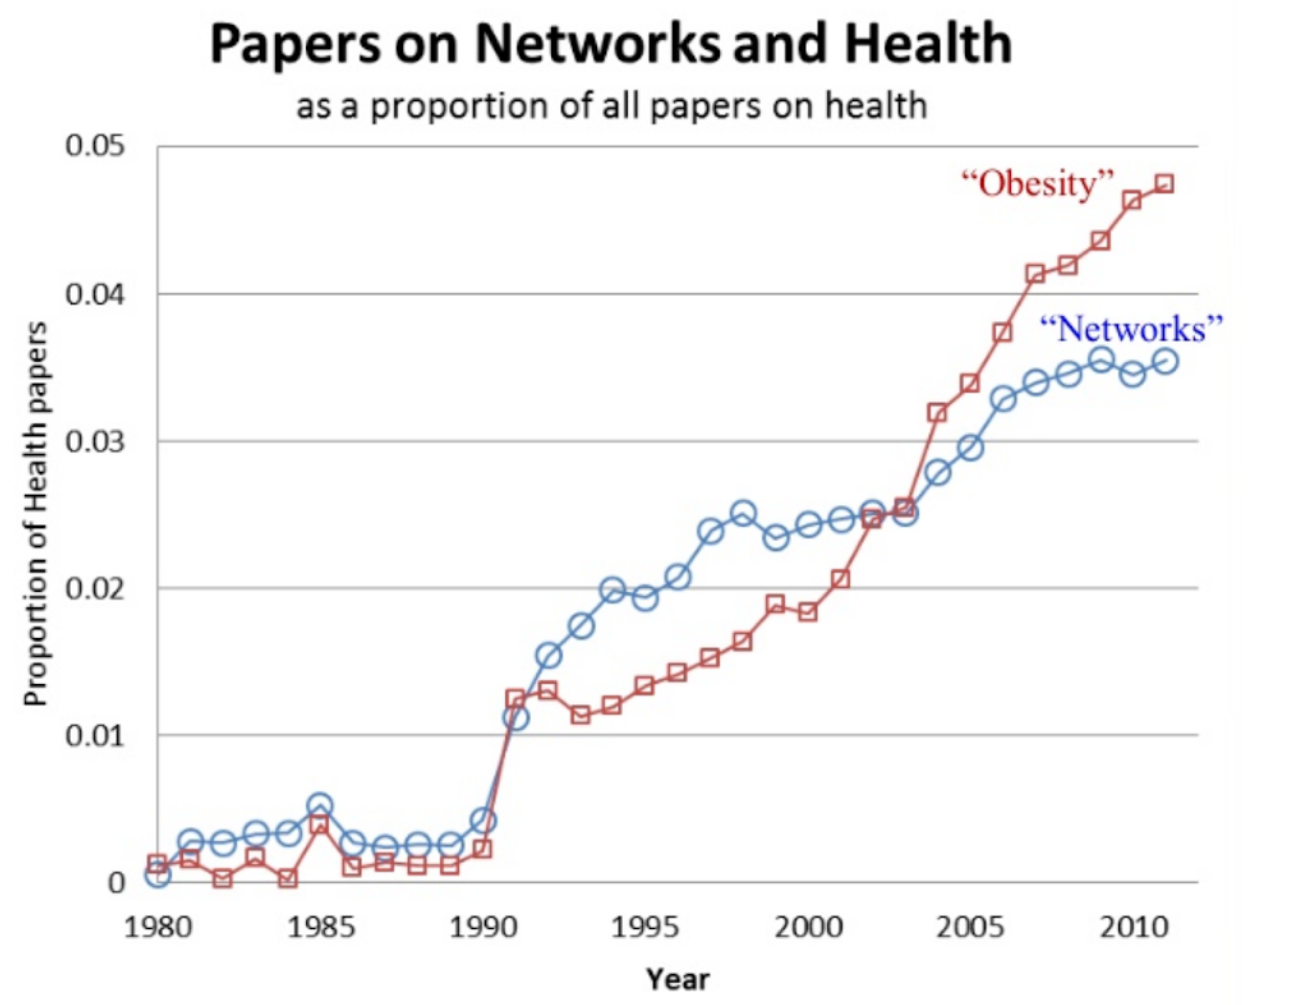
\includegraphics[width=0.7\linewidth]{figures/Networks/papersSocial.png} 
        \caption{Proportion of papers published about networks on the topic of health across the years, in comparison with the number of papers published on obesity. Reproduced from \url{https://www.sciencedirect.com/referencework/9780080970875/international-encyclopedia-of-the-social-and-behavioral-sciences}}
        \label{figure:networkNetworkRise}
    \end{figure}

Graphs provide an abstract representation of the relationships between objects, which may be used to find paths, network flow, connectivity, and more which we will discuss later on. In this context, we are going to talk about graphs and networks interchangeably. 

A graph has the following mathematical definition: \label{eq:graph}
    \begin{equation}
        G = (V,E) 
    \end{equation}
Where G is the graph, V is the set of vertices, and E is the set of edges. In figure \ref{figure:networkExampleBasic}, we define G as V = \{A, B, C, D, E, F, G, H, I, J\} and E = \{ \{A,D\}, \{B,C\}, \{C,A\}, \{C,B\}, \{D,G\}, \{E,D\}, \{F,G\}, \{F,I\}, \{G,F\}, \{H,G\}, \{J,F\} \}

\subsection{ Nodes }

A node or vertex is the fundamental element of a network. Is usually represented as a point with lines, known as edges, coming out of it, which connect it with other nodes in the network. Each node represents one elemental object in the network, which in our case is a total of 1038 students. In other contexts can be cities, computers, or any other concept.

Mathematically, we notate all nodes as V, with each individual node in a graph with lowercase variables, such as x, y, or z. The total number of nodes is notated with $|V|$. In figure \ref{figure:networkExampleBasic}, we have 10 nodes.

\subsubsection{Attributes}

Each node may have different variables, such as sex, BMI, or any other intrinsic variable proper to the object the node is representing. Each of these variables is known as the attributes of a node. Each attribute of a node is notated with subindexes, such as $x_1$, $x_2$, ... , $x_i$ , ... , $x_n$ . In figure \ref{figure:networkExampleBasic}, $A_{color} = blue$

\subsection{Edges}

An edge represents a relationship between two nodes. Our network represents a relationship of undirected friendship. The assessment of the edges is formally introduced in detail in section \cite{method:SocialNetwork}. For now, let's just comment that we have 5 types of relationships that represent the social interactions that happen between students. One is physical relationships, relationships at school, at home, at sports practice, and finally by other types of interaction. If we combine all possible edges, then we form a 6th network which we call the overall network.

Two nodes can have multiple edges with the same or different weights between them, or have none. If all edges in the graph have at least one connection to every other node, then is called a complete graph.

The mathematical definition of all edges in a graph is as follows:
    \begin{equation}
        E \subseteq  \left\{   (x,y) | (x,y) \in V^2  \land x  \neq y  \right\}
    \end{equation}
We denote the total number of edges as $|E|$. A particular edge between two nodes is simply (x,y). In figure \ref{figure:networkExampleBasic}, we have 11 edges that are directed, and in figure \ref{figure:networkExampleWeights} we have 9 edges that are undirected.

\subsubsection{Directionality}

Directionality refers to whether the edges are directed or undirected. In the case of friendship, a student may nominate others as friends while none of them nominate him back. Or they might have a strong friendship between them so everyone reciprocates everybody. Nodes can be referred to as "Ego" or "Alter". An Ego node is the node from which the relationship is emanating, and an Alter node is the node that is receiving the relationship. A phrase such as "Ego-perceived friends" means that we are focusing on a node (ego) and this node has nominated some friends.

In our network, edges are undirected, meaning that it doesn't matter which student nominates whom as a friend, in either case, there is a relationship between them.

    \begin{figure}[H]
        \centering
            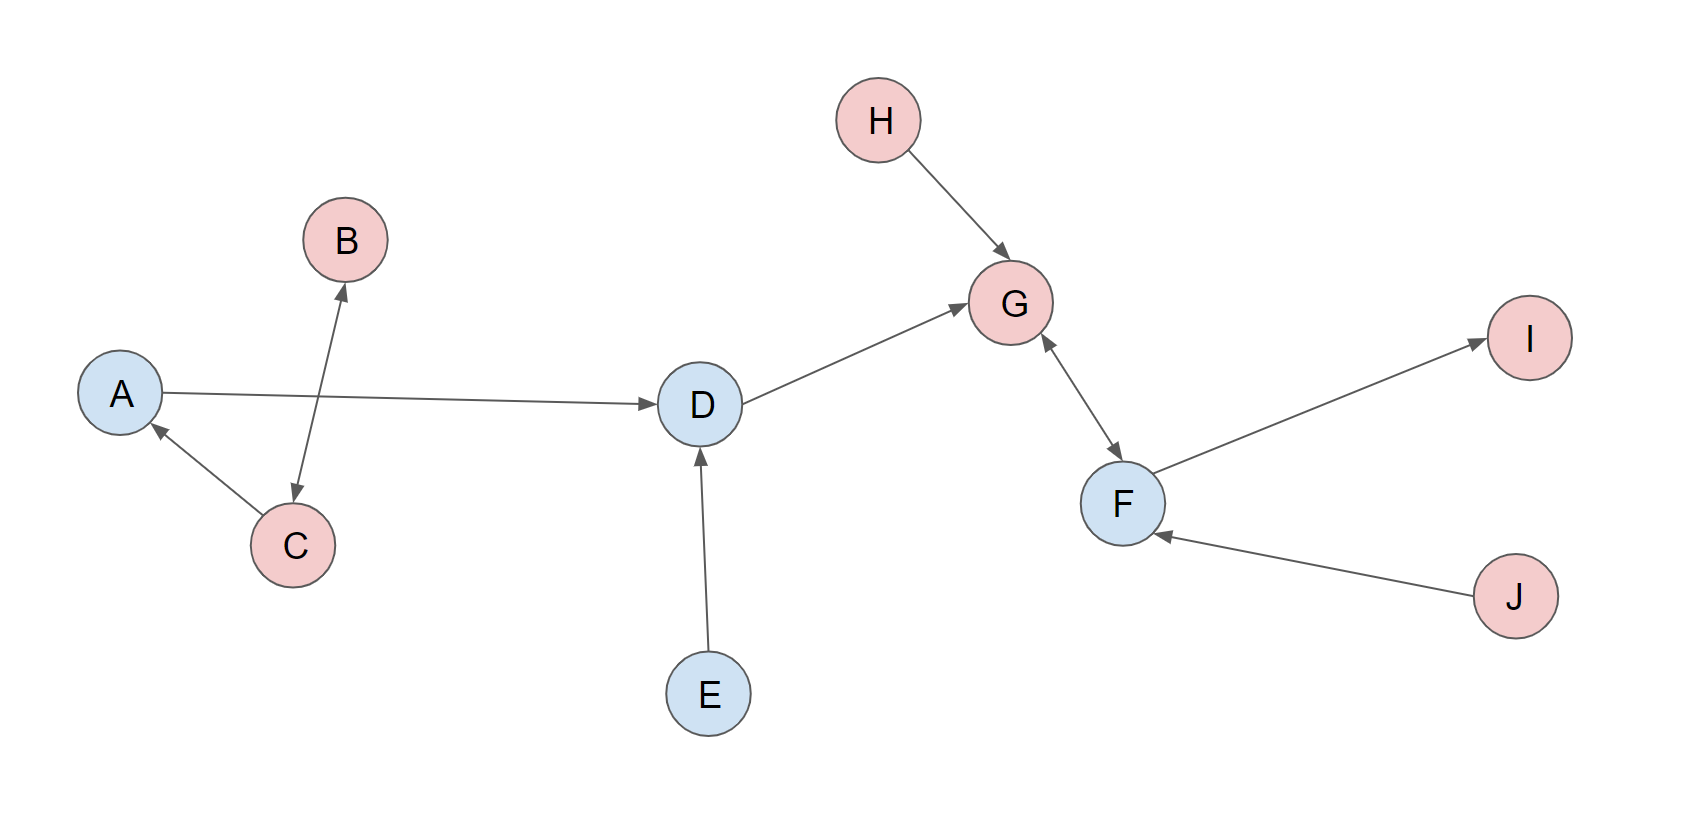
\includegraphics[width=0.7\linewidth]{figures/Networks/Concepts/directed.png} 
        \caption{An example of a network with 10 nodes labeled from A to J. Each node has a color attribute that can be either red or blue. Nodes are connected via directed relationships. Nodes B and C, and nodes G and F have a reciprocal relationship. The Laplacian representation of this matrix can be seen in table \ref{table:networkLaplacian}}
        \label{figure:networkExampleBasic}
    \end{figure}

    \begin{figure}[h!]
        \centering
            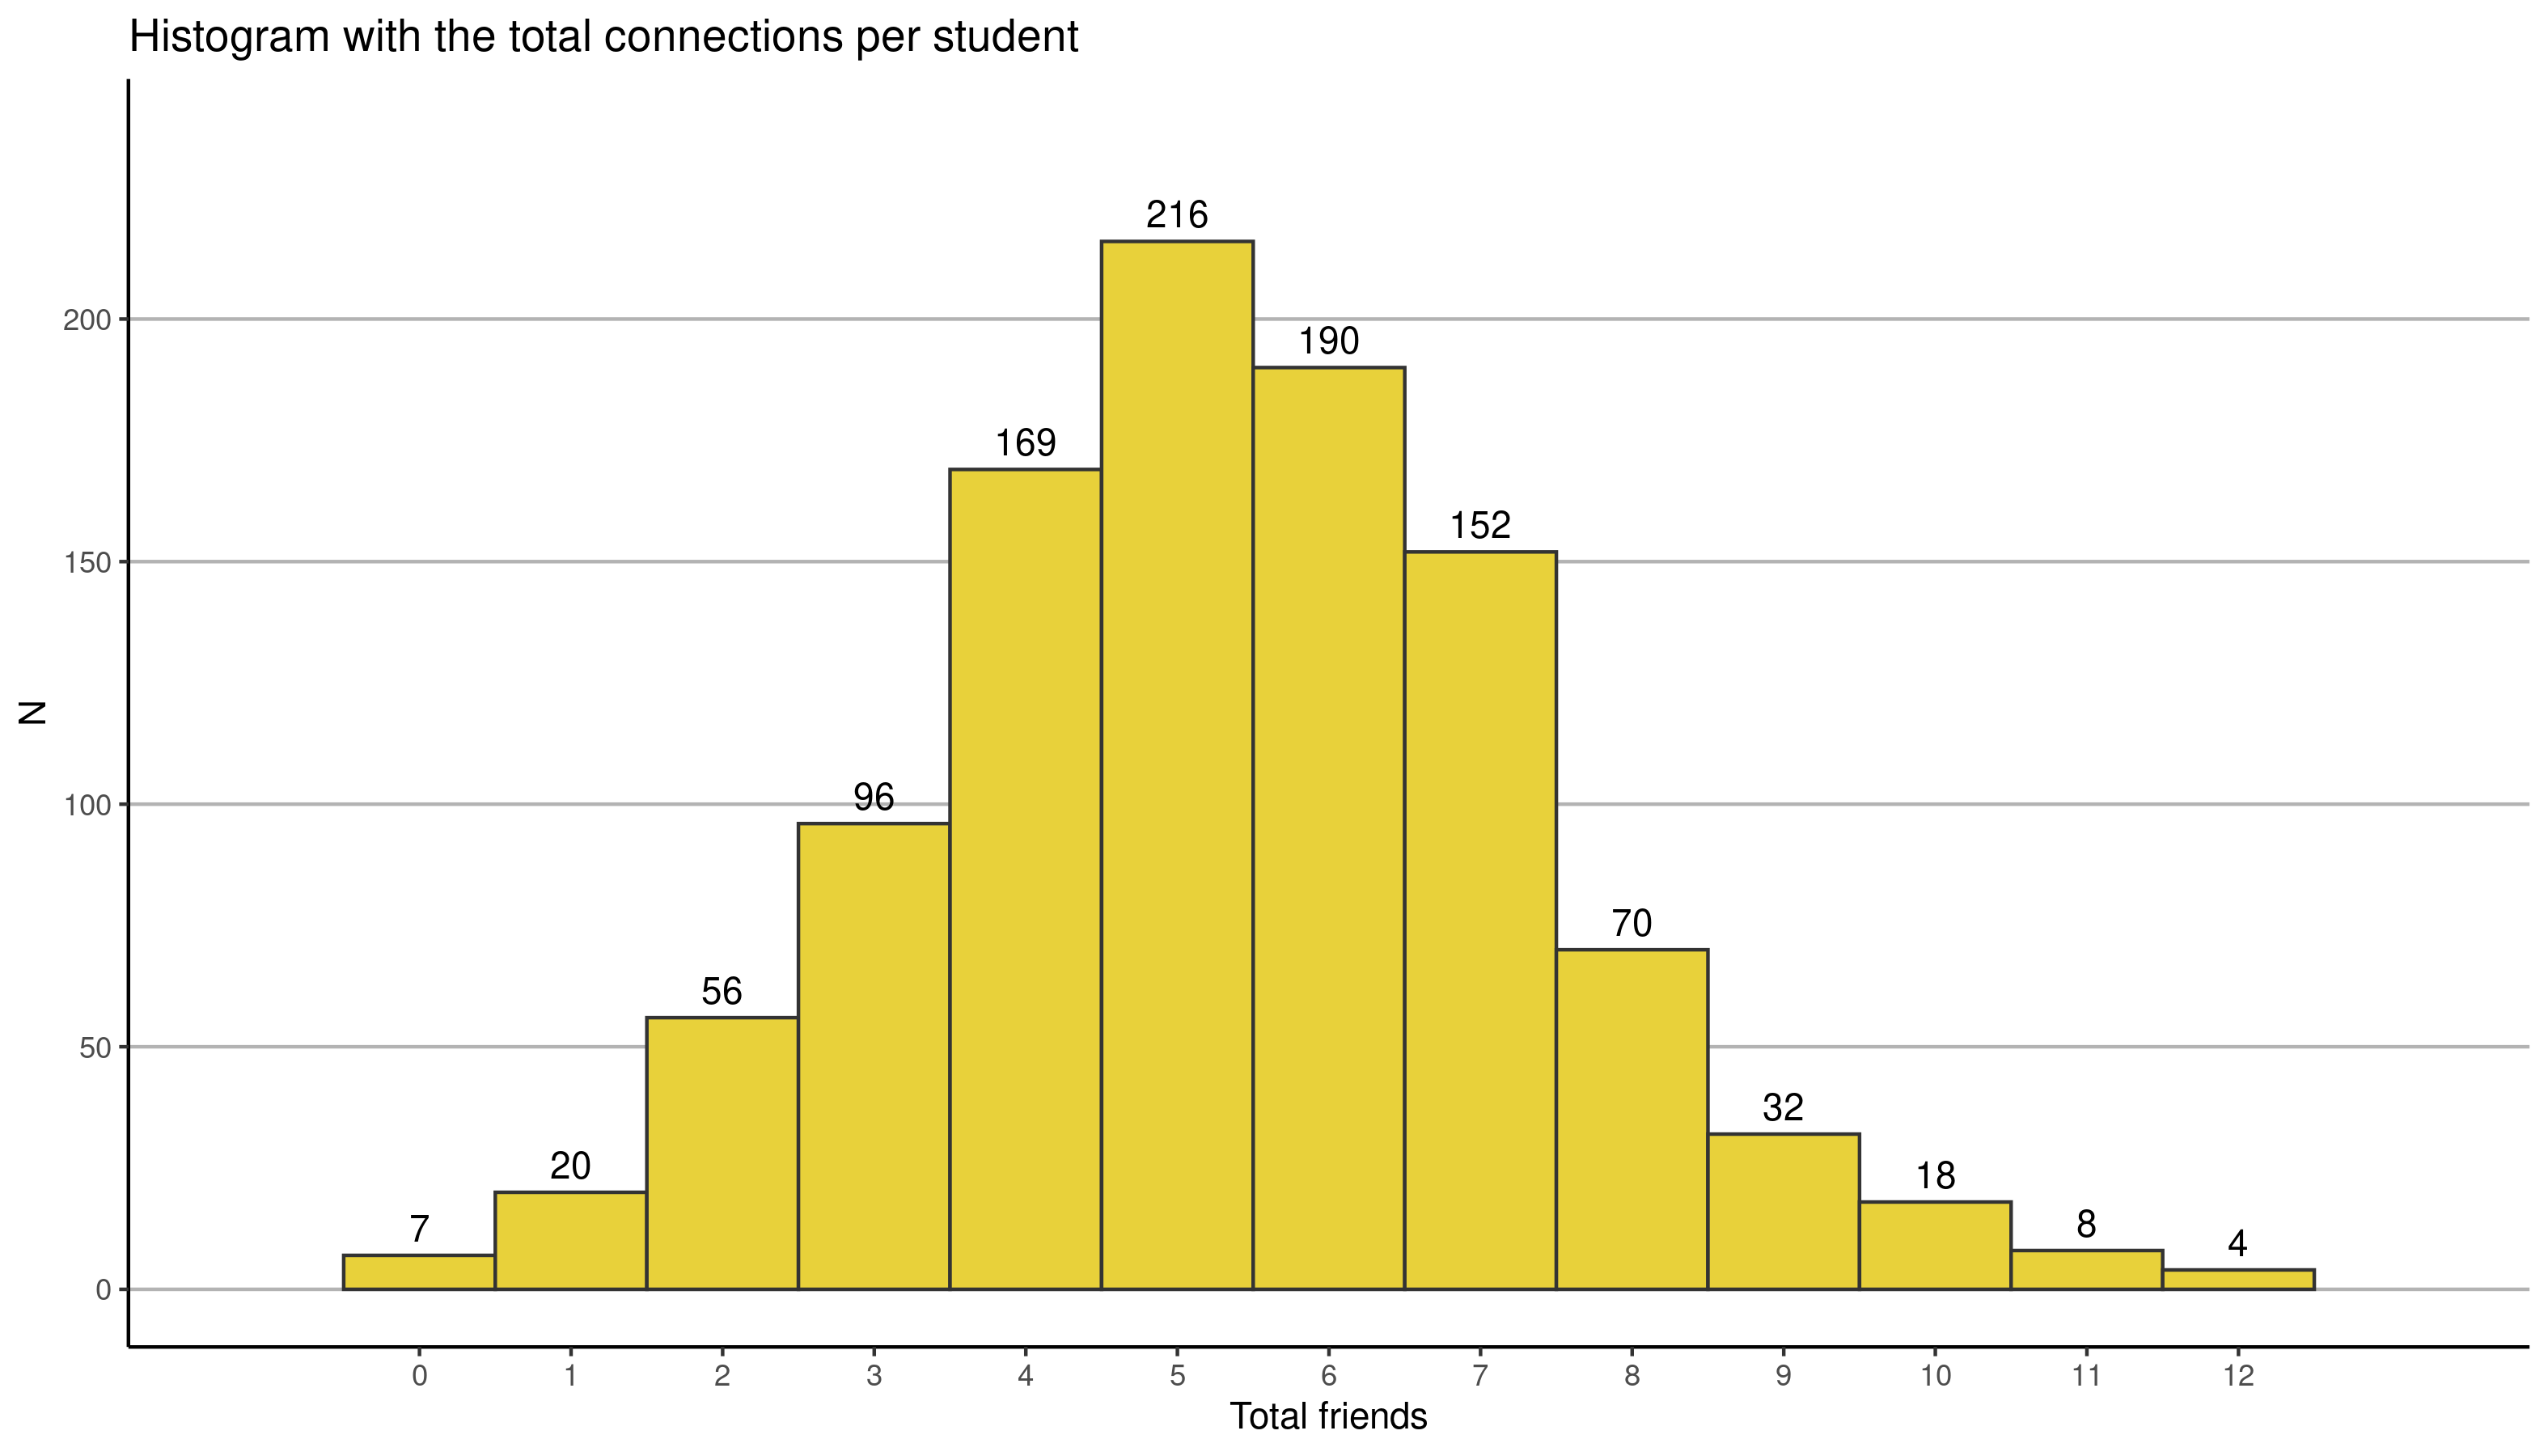
\includegraphics[width=0.7\linewidth]{figures/Networks/Histograms/Histogram_completeTable_OverallConnections.png} 
        \caption{A histogram with the total of undirected friends per student in the overall network. Some students are popular with up to 12 connections, while others are isolated with 0 connections.}
        \label{figure:networksHistogramFriendship}
    \end{figure}  

\subsubsection{Reciprocity ratio}

The reciprocity ratio is the number of edges that has a reciprocal relationship. This can only be measured in networks that are directed.

\subsubsection{Weight}

All edges have an additional property called weight. This is a variable, typically a real number, that indicates some quantifying property of the relationship. For example the distance between two cities, or how many hours per day you spend in the company of a person. By default, all edges have a weight of 1, meaning all relationships have the same importance; this is our case study.

    \begin{figure}[h!]
        \centering
            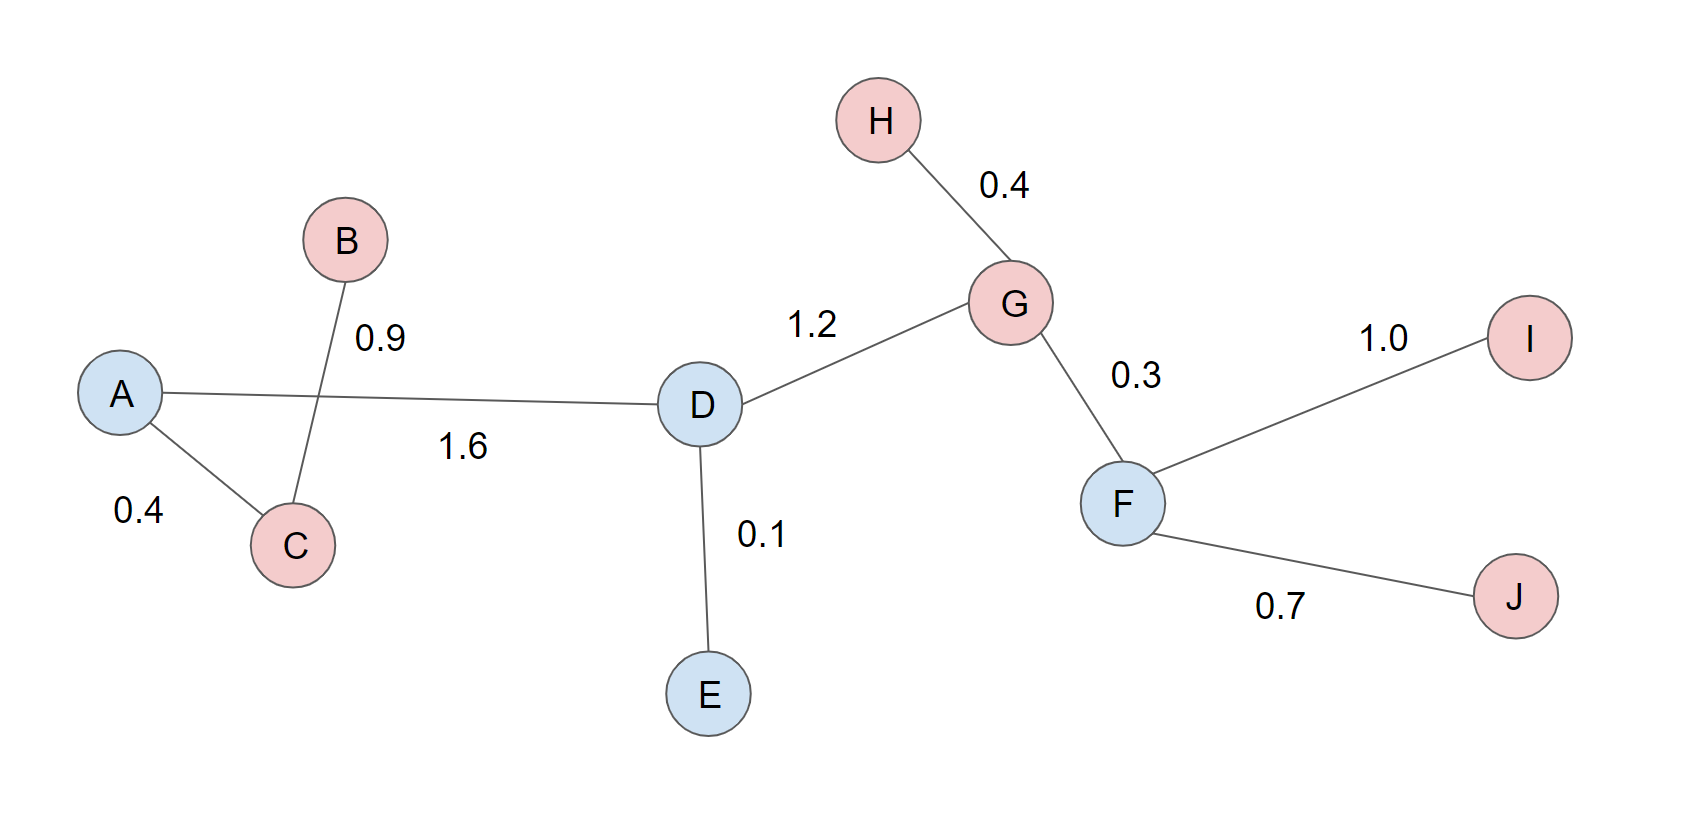
\includegraphics[width=0.7\linewidth]{figures/Networks/Concepts/edgesValues.png} 
        \caption{An example of a network with 10 nodes and weighted undirected relationships. A spring layout of this network can be seen in figure \ref{figure:networkExampleSpring}}
        \label{figure:networkExampleWeights}
    \end{figure}

Nodes that are not connected can be defined to either have a weight of zero or a weight of infinity, depending on the wording of your definition.

\subsubsection{Loop}

A relationship of a node with itself is allowed in graph theory and is called a loop. Be aware that this may not make sense in a context such as ours. Philosophically a person might be friends with himself if we define it as being happy with his life, but mathematically we don't have any use for such a definition. But it can make sense if we talk about a network of collaborations and we define a loop as authors' self-promotion. In a transportation network, a loop can represent a roundabout where a vehicle can circle around the same point.

\subsubsection{Connectivity}
\label{network:Connectivity}

Is the summation of all edges' weight. When all the nodes in the network have at least 1 connectivity is it said that the network is fully connected. There are four main methods of measuring connectivity:

\begin{itemize}
    \item \textbf{In-degree:} Summation of all the weights coming into the node.
    \item \textbf{Out-degree:} Summation of all the weights going outside the node.
    \item \textbf{Reciprocity:} Summation of weights in reciprocal edges.
    \item \textbf{Undirected:} Summation of in and out connections.
\end{itemize}

    \label{table:networkGeneralStats}
    \begin{table}[h!]    
        \centering
        \caption{Overview of all basic statistics of the six networks. From left to right, the name of the network, the total number of edges in the network, average out-degree, average in-degree, average reciprocity, the average number of connections per node, and the average distance between non-isolated nodes. Notice that average out-degree and average in-degree must have the same value, but the standard deviation varies. Reciprocity in "Overall" is increased because nodes can nominate in one network but receive the nomination from the same friend from another network.}
        \footnotesize
        \renewcommand{\arraystretch}{1.7}
            \begin{tabular}{r|rrrrrr} 
            \hline
            
            \rowcolor[rgb]{1,1,0.78} \multicolumn{1}{c}{Name} & \multicolumn{1}{c}{Edges} & \multicolumn{1}{c}{$\overline{Out}$} & \multicolumn{1}{c}{$\overline{In}$} & \multicolumn{1}{c}{$\overline{Reciprocity}$} & \multicolumn{1}{c}{$\overline{Connections}$} & \multicolumn{1}{c}{$\overline{Distance}$}  \\ 
            \hline
            
            {\cellcolor[rgb]{1,0.808,0.576}}Overall           & 3767              & 3.63 ± 1.32 & 3.63 ± 2.11 & 1.92 ± 1.27 & 5.34 ± 2.04 & 8.00                                        \\
            {\cellcolor[rgb]{1,0.808,0.576}}Physical          & 2823              & 2.72 ± 1.71 & 2.72 ± 1.96 & 1.25 ± 1.20 & 4.18 ± 2.19 & 9.91                                     \\
            {\cellcolor[rgb]{1,0.808,0.576}}School            & 2979              & 1.20 ± 1.35 & 1.20 ± 1.25 & 0.49 ± 0.75 & 1.92 ± 1.66 & 6.90                                      \\
            {\cellcolor[rgb]{1,0.808,0.576}}Sport             & 598               & 2.87 ± 1.59 & 2.87 ± 1.85 & 1.42 ± 1.20 & 4.32 ± 1.92 & 13.73                                    \\
            {\cellcolor[rgb]{1,0.808,0.576}}Home              & 1247              & 0.58 ± 1.11 & 0.58 ± 1.04 & 0.18 ± 0.56 & 0.97 ± 1.48 & 3.58                                     \\
            {\cellcolor[rgb]{1,0.808,0.576}}Other             & 1095              & 1.05 ± 1.47 & 1.05 ± 1.11 & 0.26 ± 0.58 & 1.85 ± 1.68 & 7.08                                    
            \end{tabular}
    \end{table}

\subsubsection{Laplacian matrix}

A graph can be represented as a matrix, in which each cell combination of row and column represents an edge between two nodes. This is known as the Laplacian matrix of a graph, or simply the matrix.

\label{table:networkLaplacian}
\begin{table}[h!]

    \centering

    \caption{Example of a Laplacian matrix corresponding to figure \ref{figure:networkExampleBasic}. Summation by row represents the out-degree. Summation by columns represents the in-degree. Cells that are symmetrical from the main diagonal, represent reciprocal relationships.}
    
    \begin{tabular}{|c|cccccccccc|} 
    \hhline{~----------|}
    \multicolumn{1}{c|}{}           & \multicolumn{10}{c|}{{\cellcolor[rgb]{1,0.988,0.62}}Node receiving the edge}                                                                                                                                                                                                                                         \\ 
    \hhline{~----------|}
    \multicolumn{1}{c|}{}           & {\cellcolor[rgb]{1,1,0.78}}A & {\cellcolor[rgb]{1,1,0.78}}B & {\cellcolor[rgb]{1,1,0.78}}C & {\cellcolor[rgb]{1,1,0.78}}D & {\cellcolor[rgb]{1,1,0.78}}E & {\cellcolor[rgb]{1,1,0.78}}F & {\cellcolor[rgb]{1,1,0.78}}G & {\cellcolor[rgb]{1,1,0.78}}H & {\cellcolor[rgb]{1,1,0.78}}I & {\cellcolor[rgb]{1,1,0.78}}J  \\ 
    \hline
    {\cellcolor[rgb]{0.604,1,0.6}}A & 0                            & 0                            & 0                            & 1                            & 0                            & 0                            & 0                            & 0                            & 0                            & 0                             \\
    {\cellcolor[rgb]{0.604,1,0.6}}B & 0                            & 0                            & 1                            & 0                            & 0                            & 0                            & 0                            & 0                            & 0                            & 0                             \\
    {\cellcolor[rgb]{0.604,1,0.6}}C & 1                            & 1                            & 0                            & 0                            & 0                            & 0                            & 0                            & 0                            & 0                            & 0                             \\
    {\cellcolor[rgb]{0.604,1,0.6}}D & 0                            & 0                            & 0                            & 0                            & 0                            & 0                            & 1                            & 0                            & 0                            & 0                             \\
    {\cellcolor[rgb]{0.604,1,0.6}}E & 0                            & 0                            & 0                            & 1                            & 0                            & 0                            & 0                            & 0                            & 0                            & 0                             \\
    {\cellcolor[rgb]{0.604,1,0.6}}F & 0                            & 0                            & 0                            & 0                            & 0                            & 0                            & 1                            & 0                            & 1                            & 0                             \\
    {\cellcolor[rgb]{0.604,1,0.6}}G & 0                            & 0                            & 0                            & 0                            & 0                            & 1                            & 0                            & 0                            & 0                            & 0                             \\
    {\cellcolor[rgb]{0.604,1,0.6}}H & 0                            & 0                            & 0                            & 0                            & 0                            & 0                            & 1                            & 0                            & 0                            & 0                             \\
    {\cellcolor[rgb]{0.604,1,0.6}}I & 0                            & 0                            & 0                            & 0                            & 0                            & 0                            & 0                            & 0                            & 0                            & 0                             \\
    {\cellcolor[rgb]{0.604,1,0.6}}J & 0                            & 0                            & 0                            & 0                            & 0                            & 1                            & 0                            & 0                            & 0                            & 0                             \\
    \hline
    \end{tabular}
\end{table}

%https://en.wikipedia.org/wiki/Laplacian_matrix

\subsubsection{Distance}

A distance is the summation of the edge's weights between two nodes, whether they are directly connected or have some intermediary nodes between them. Distance is not necessarily unique, a couple of nodes can have several different distances between them. If two nodes have no connection, the distance is equal to infinity. If your network allows for edges forming loops then you will also have an infinite combination of nodes and thus infinite possible distances.

\subsubsection{Path}

A path is the minimum weighted distance between two nodes. The path to the same node can be 0, or another value specified in a loop. A path can be negative if the graph is allowed to have negative distances. A path can be infinite if, for example, two nodes are unreachable from one to another. A directed graph can have different path lengths from any given pair of two nodes.

    \begin{figure}[h]
        \centering
            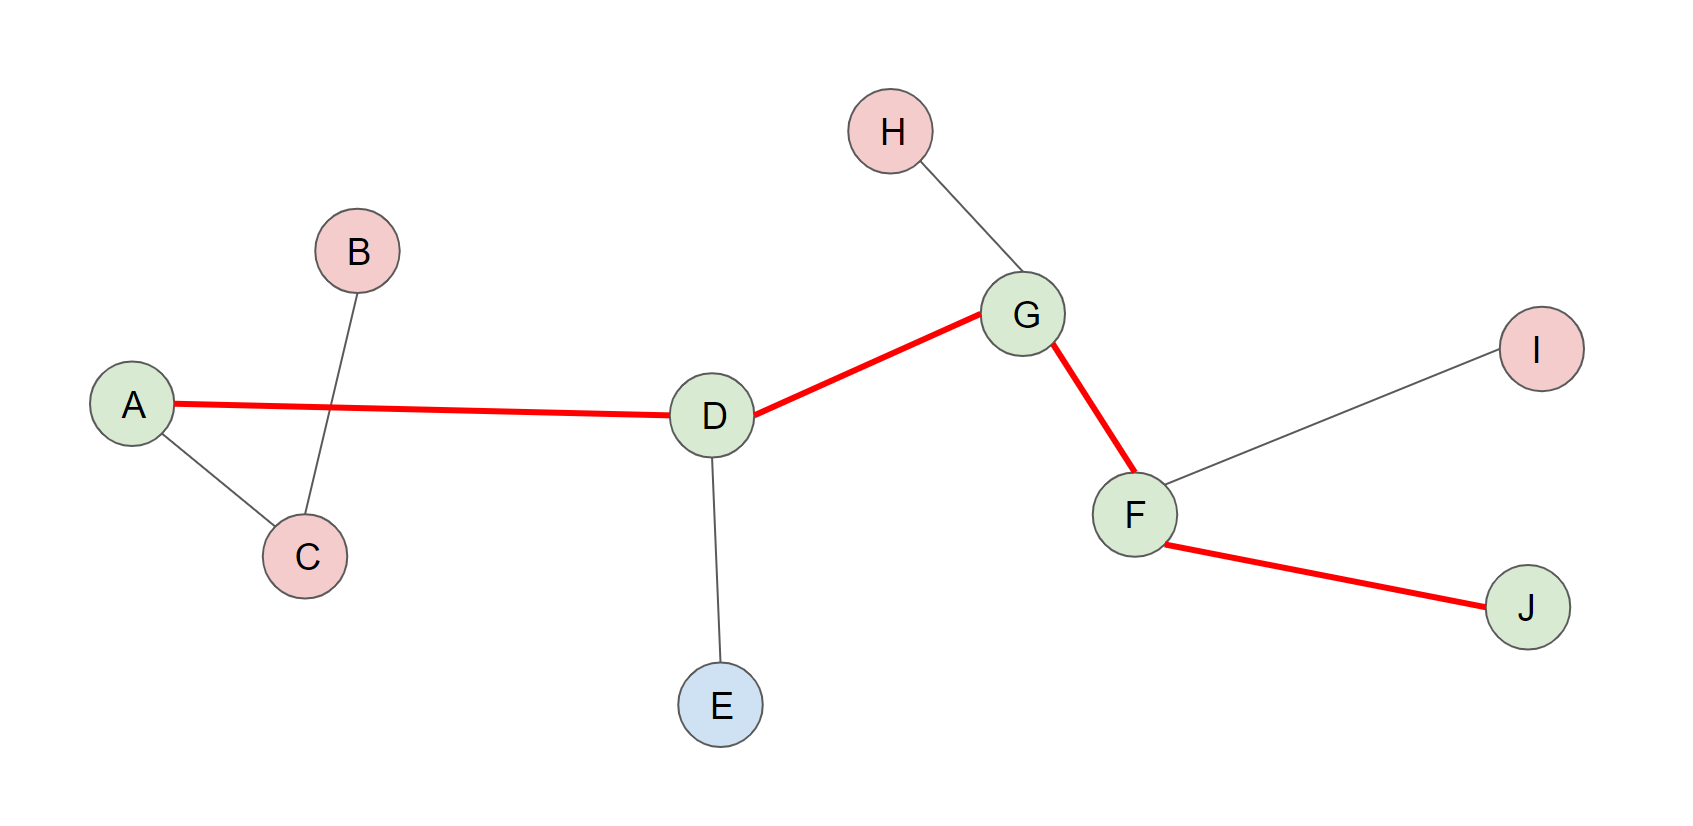
\includegraphics[width=0.7\linewidth]{figures/Networks/Concepts/path.png} 
        \caption{An example of a path. Node A can reach node J following the red highlighted edges and passing through the green highlighted nodes. All the edges weigh the same value (1), so the path is equal to 4.}
        \label{figure:networkPath}
    \end{figure}

\subsection{Network}

%https://eehh-stanford.github.io/SNA-workshop/graphs.html#dyads-triads-and-other-local-structures

% https://www.cambridge.org/core/books/abs/social-network-analysis/dyads/52A3652CD28CA469BA95572A1B714EC3 Book about social network for references.

% ERGM models, there is nothing done with this https://appliednetsci.springeropen.com/articles/10.1007/s41109-021-00403-5

\subsubsection{Isomorphic}
\label{network:isomorphic}

Two graphs are said to be isomorphic if they have the same edges and nodes if we remove the attributes of all nodes in both graphs. This is also known as network topology.

\subsubsection{Network motifs}

A set of two nodes is called a diad. A set of three nodes is called a triad. A set of four nodes is called a tetrad. An undirected diad can have only two states, either the two nodes share an edge, or they don't. A directed diad can have 4 states: no common edge, the edge from A to B, the edge from B to A, reciprocal edges from A to B, and B to A. Similarly, triads and tetrads have a limited amount of combinations of edges and no edges between their nodes. All of these examples are called network motifs.

Networks that have the same context, for example, how animals share spaces in the wilderness, and how followers are distributed in internet social networks, tend to have the same distribution of motifs. Sometimes is useful to compare the motif count with other network motif counts to check if their structure is similar. Other time is interesting to simulate a network by giving a set of probabilities for each network motif to force a specific structure.

Network motifs are an important concept in social science studies to describe the structure of the network \cite{Faust2010}, but there are better metrics on how to describe a network \cite{Faust2007}.

\subsubsection{Components}

 If no path exists that connects all nodes with all other nodes in the network it means that you have a network divided into components. A network can have isolated nodes, isolated diads, triads, or be divided into several sub-networks. Each of these cases is known as a component of a network. In figure \ref{figure:networksConnectivity} we have one network with two components. 

\subsubsection{Clusters and Communities}

Community detection is the process of discovering groups or clusters of nodes in a social network that have a high degree of connectivity within themselves, or low with other groups. There is no best algorithm and the use of each depends on the needs of the researcher:

\begin{itemize}

    \item \textbf{Modularity:} This method compares the density of different groups and is useful to compare hierarchical and overlapping communities.
    
    \item \textbf{Clustering:} This is a family of algorithms that consists of dividing groups with similar attributes. Different approaches are k-means, hierarchical clustering, or spectral clustering
    
    \item \textbf{Link-based:} This method uses the edges in the graph and measures how far you can walk from one node to another one. Communities tend to have shorter walking distances between them.

    \item \textbf{Latent variable:} These methods are somewhat similar to PCA analysis, in which we decided a number of hidden latent variables, and the algorithm groups automatically nodes based on those latent variables.

\end{itemize}

In our case, we already have the data divided in communities by high schools, down to the same class levels. And we have several attributes in each node to compare different values. As we have not done any study regarding the intricacies of each high school individually, no clustering has been applied so far other than calculating homophilies (section \ref{network:homophily}).

% https://towardsdatascience.com/an-introduction-to-graph-partitioning-algorithms-and-community-detection-29e7c962d10e?gi=ab4d5c83b911

%https://towardsdatascience.com/an-introduction-to-graph-neural-network-gnn-for-analysing-structured-data-afce79f4cfdc

% https://appliednetsci.springeropen.com/articles/10.1007/s41109-019-0248-7

% Prostitutes in China Moody, James, Jimi Adams, and Martina Morris. “Epidemic potential by sexual activity distributions.” Network Science (Cambridge University Press) 5, no. 4 (December 2017): 461–75.

% https://stackoverflow.com/questions/9471906/what-are-the-differences-between-community-detection-algorithms-in-igraph/

% https://www.r-bloggers.com/2012/06/summary-of-community-detection-algorithms-in-igraph-0-6/

% https://people.duke.edu/~jmoody77/snh/2021/CommunitiesSNH2021.nb.html

\subsubsection{Multimodal networks}

The network can be multimodal. This means that a node can connect to other nodes that are not of the same class. For example, a researcher can collaborate with other researchers, which are nodes of the same class. They publish a paper together which is another class of nodes that nevertheless connect to researchers. The paper is published in a journal which is another class. Multimodal networks are characterized as being hard to analyze due to the different meanings of the different relationships.

\section{Layout}

So far we can define a network as a table of nodes with attributes, and another table of edges and weights. Mathematically this is all we need. But for visualization purposes, there are several possibilities as to how we can spread the nodes in a typically 2D or 3D image. Proper node placement can help in creating a clear and intuitive picture making it easier to understand the relationships between the nodes. On the other hand, the emerging pattern in the network can be hidden if a poor option is chosen. This is called network layout. There are several algorithms for vertex placement. The basic categories are:

    \begin{figure}[H]
        \centering
            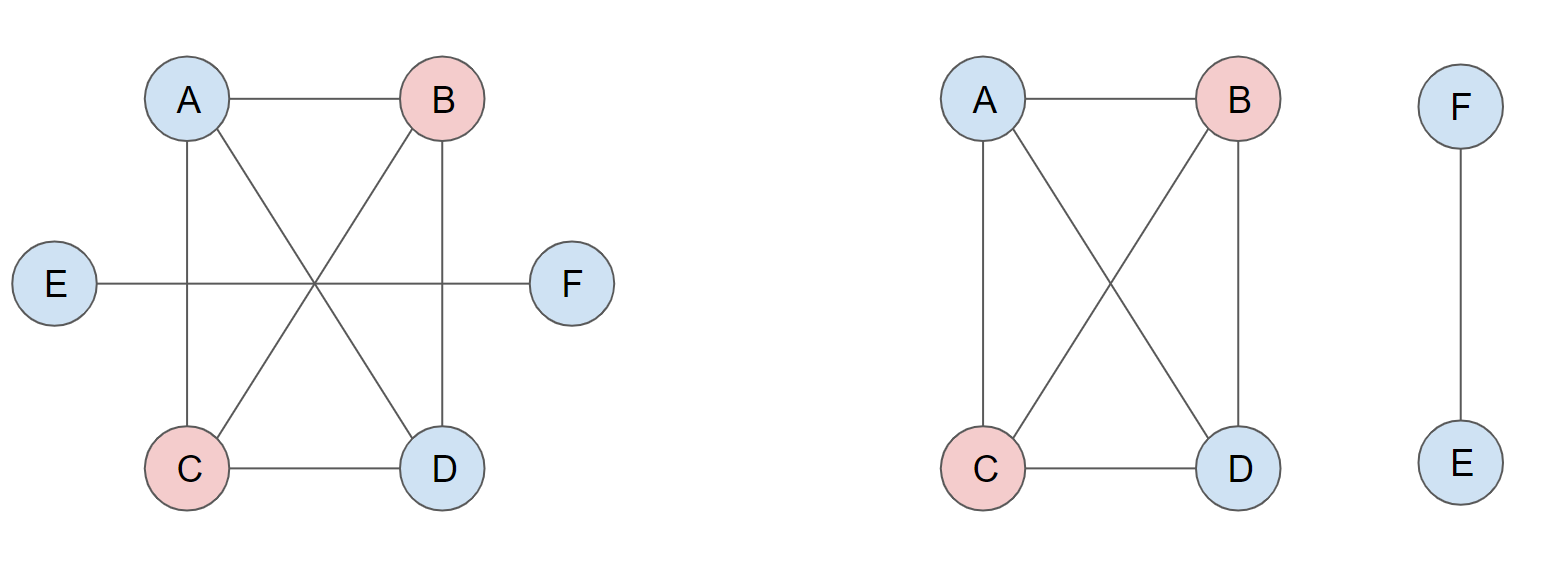
\includegraphics[width=0.7\linewidth]{figures/Networks/Layouts/isomorp.png} 
        \caption{An example of two layouts. On the left, the relationship between E and F is not clear. On the right, is obvious that E and F are disconnected from all other nodes}
        \label{figure:networkExampleLayout}
    \end{figure}

\subsection{Random}

Random placement of the nodes. Just spread the nodes around in no particular order and hope for the best.

    \begin{figure}[H]
        \centering
            \includegraphics[width=0.7\linewidth]{figures/Networks/Layouts/Graph_OverallNetwork_with_no_highlight_grid_HighSchool___grid.png} 
        \caption{Overall network placing the nodes randomly in a 2D grid. This is useful when the amount of connections is very low, but otherwise useless for visualizing patterns in this network.}
        \label{figure:networksLayoutsGRID}
    \end{figure}

\newpage

\subsection{Force directed}

This uses physics-based simulations to determine the position of nodes based on the attractive and repulsive forces between them. For example, we can imagine the nodes as electrical charges based on node properties, or the edges as springs with an elastic force proportional to the edge value.

    \begin{figure}[h!]
        \centering
            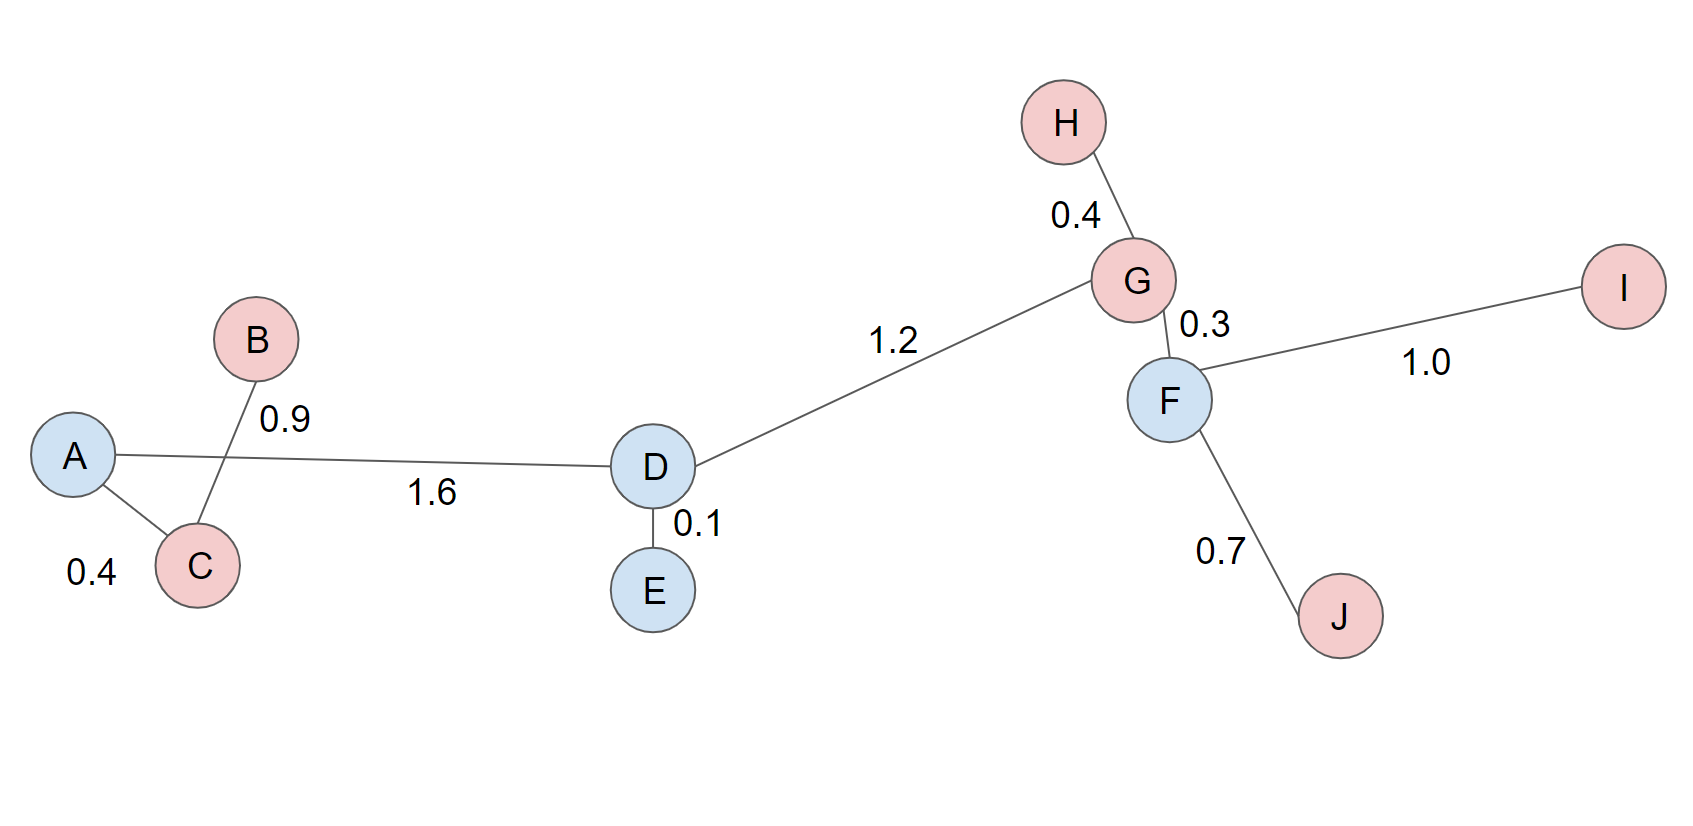
\includegraphics[width=0.7\linewidth]{figures/Networks/Concepts/edgesSpring.png} 
        \caption{An example of a network with 10 nodes and weighted undirected relationships with a spring layout. Nodes with smaller weights are brought closer together in the 2D space as if the edges were acting as springs with greater or lower spring force equilibrium alike to Hooke’s law.}
        \label{figure:networkExampleSpring}
    \end{figure}

\subsection{Hierarchical}

Hierarchical layouts tend to put important nodes on top, and less important nodes on the bottom. This type of layout only makes sense when you actually have a hierarchical relationship. Common in multi-modal networks, or where there are many triads with only two nodes connecting. Hierarchy would also mean that nodes' placement in the y-axis has some meaning of importance.

    \begin{figure}[h!]
        \centering
            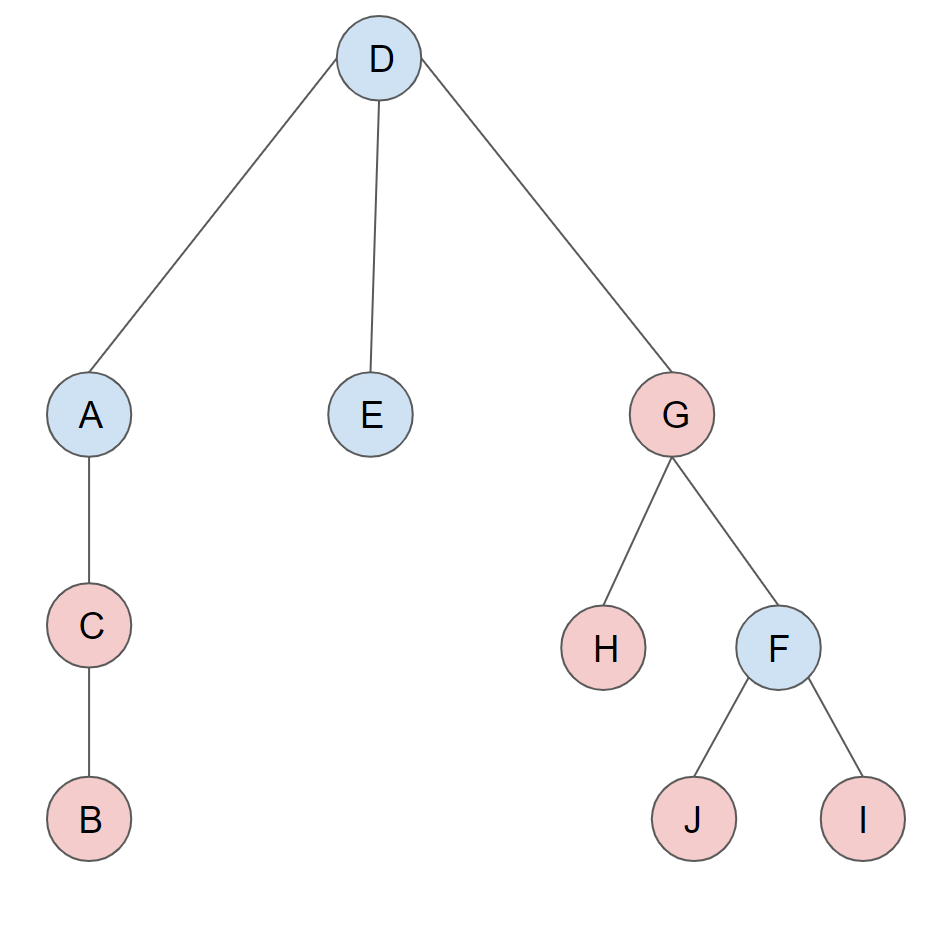
\includegraphics[width=0.5\linewidth]{figures/Networks/Layouts/hirearchy.png} 
        \caption{Our recurrent example of a network layout in a hierarchical pattern. In this example is highlighted that D is a very important node in the network, and is placed on top.}
        \label{figure:networkExampleHierarchy}
    \end{figure}

\newpage

\subsection{Spectral}

A way that minimizes a particular energy function derived from the graph's Laplacian matrix. The spectral placement technique is designed to produce graph layouts that not only look aesthetically pleasing but also provide some semantic information about the underlying network

\subsubsection{DRL}

    \begin{figure}[h!]
        \centering
            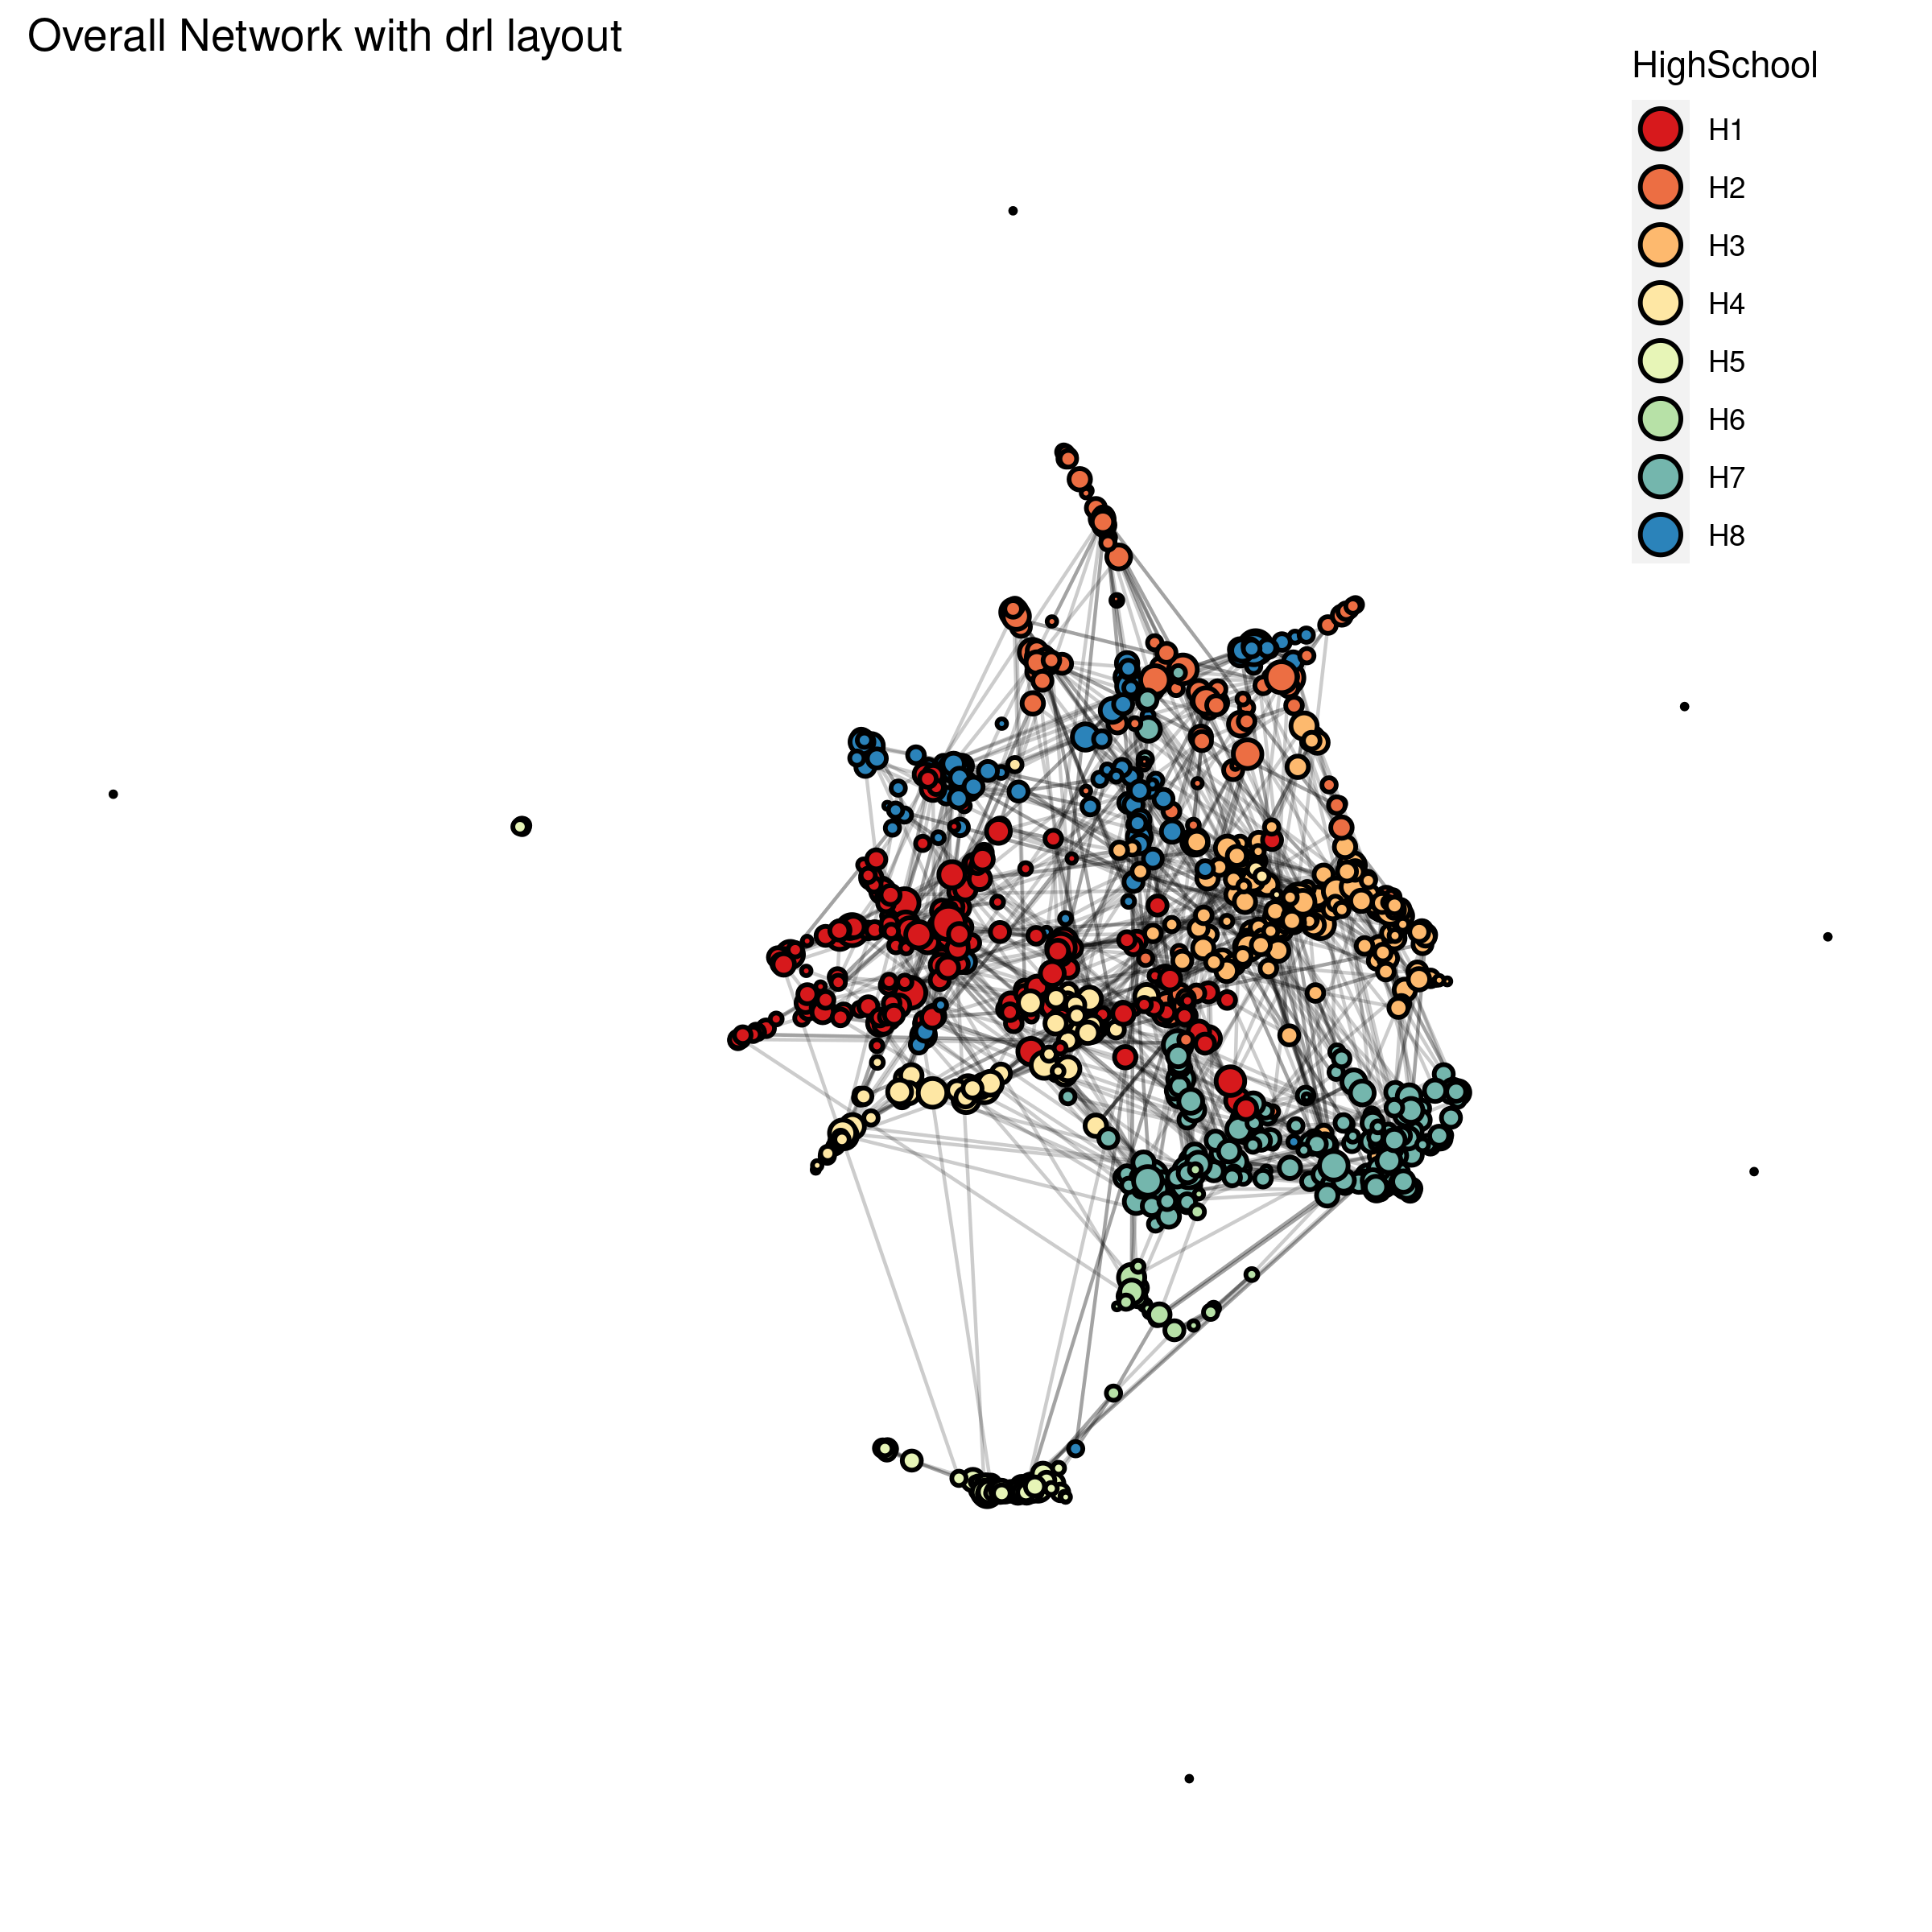
\includegraphics[width=0.7\linewidth]{figures/Networks/Layouts/Graph_OverallNetwork_with_no_highlight_drl_HighSchool___drl.png} 
        \caption{Overall network with a \gls{drl} algorithm  \cite{osti_1145621} . The layout produced by a DRL is hierarchical in nature and is well-suited for presenting large-scale graphs with a clear structure. In our case, it clusters high schools somewhat together but is not the best choice for our network.}
        \label{figure:networksLayoutsDRL}
    \end{figure}

    \newpage

\subsubsection{Fruchterman - Reingold}

    \begin{figure}[h!]
        \centering
            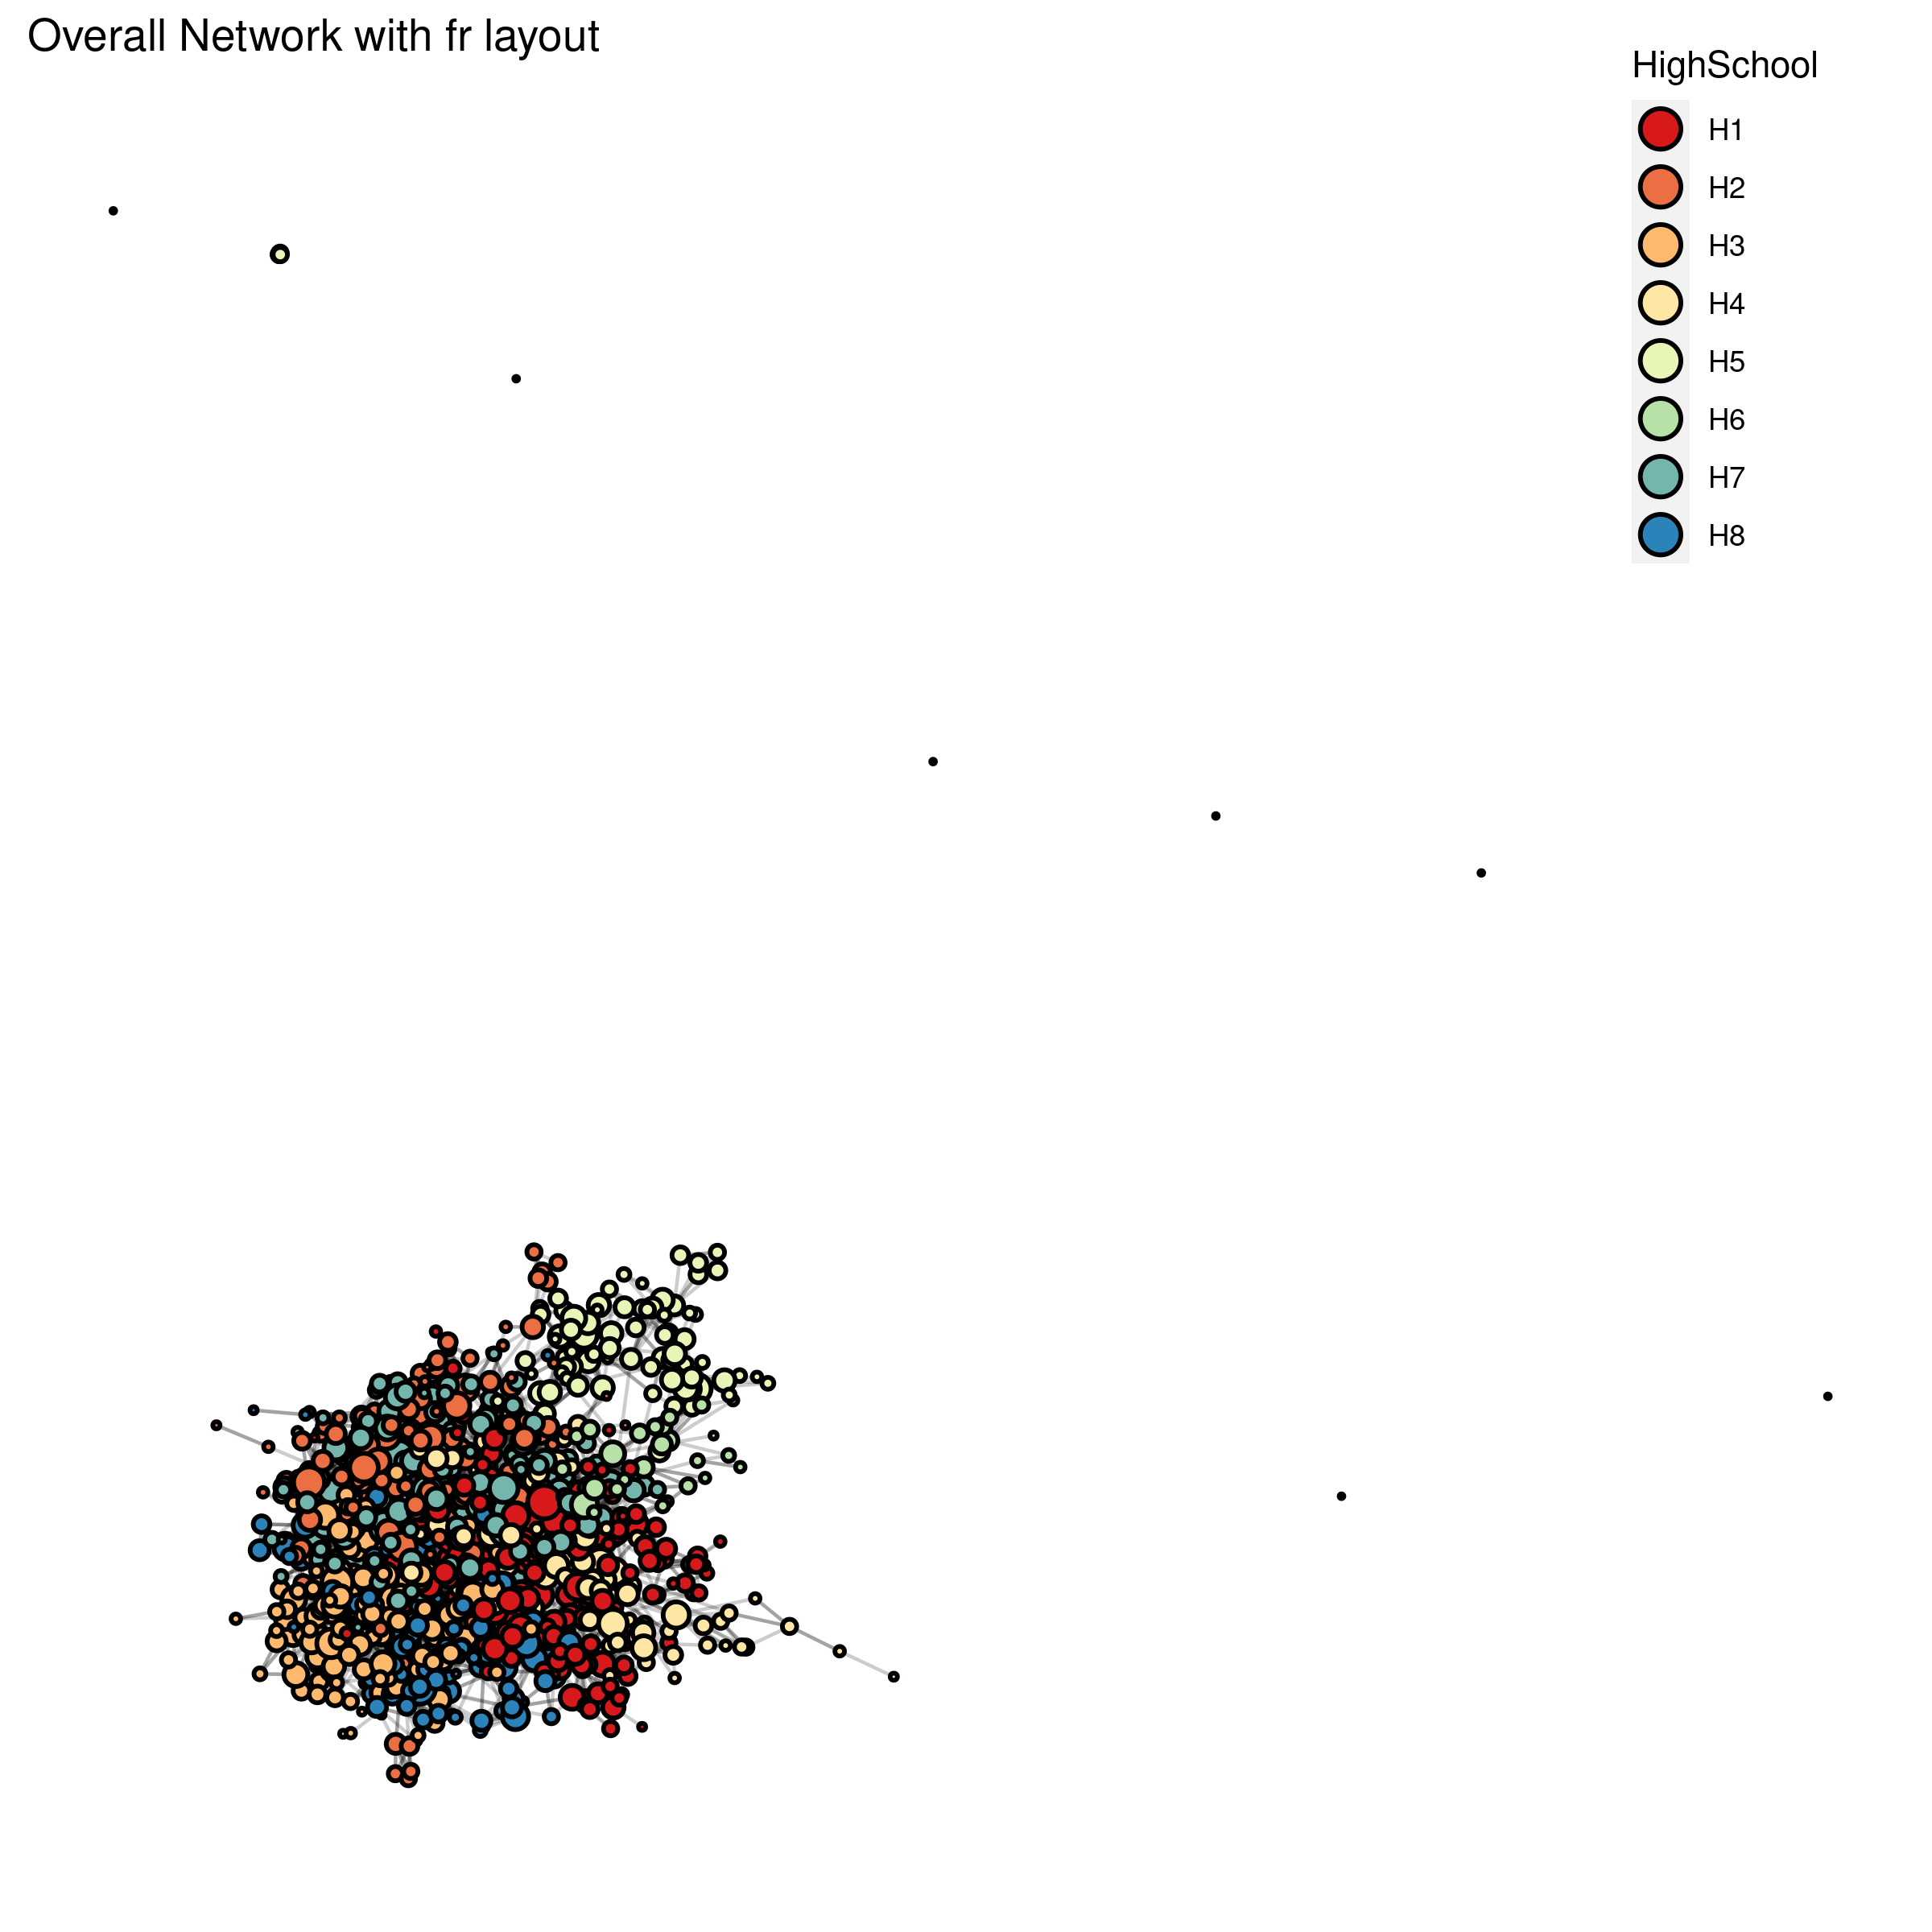
\includegraphics[width=0.7\linewidth]{figures/Networks/Layouts/Graph_OverallNetwork_with_no_highlight_fr_HighSchool___fr.png} 
        \caption{Overall network with a Fruchterman - Reingold algorithm \cite{Fruchterman1991}, it keeps related vertices together. In our case, we have some isolated nodes that are too far away, while the network is clumped in one little space. Also not good.}
        \label{figure:networksLayoutsFR}
    \end{figure}

    \newpage

\subsubsection{Graphopt}

    \begin{figure}[h!]
        \centering
            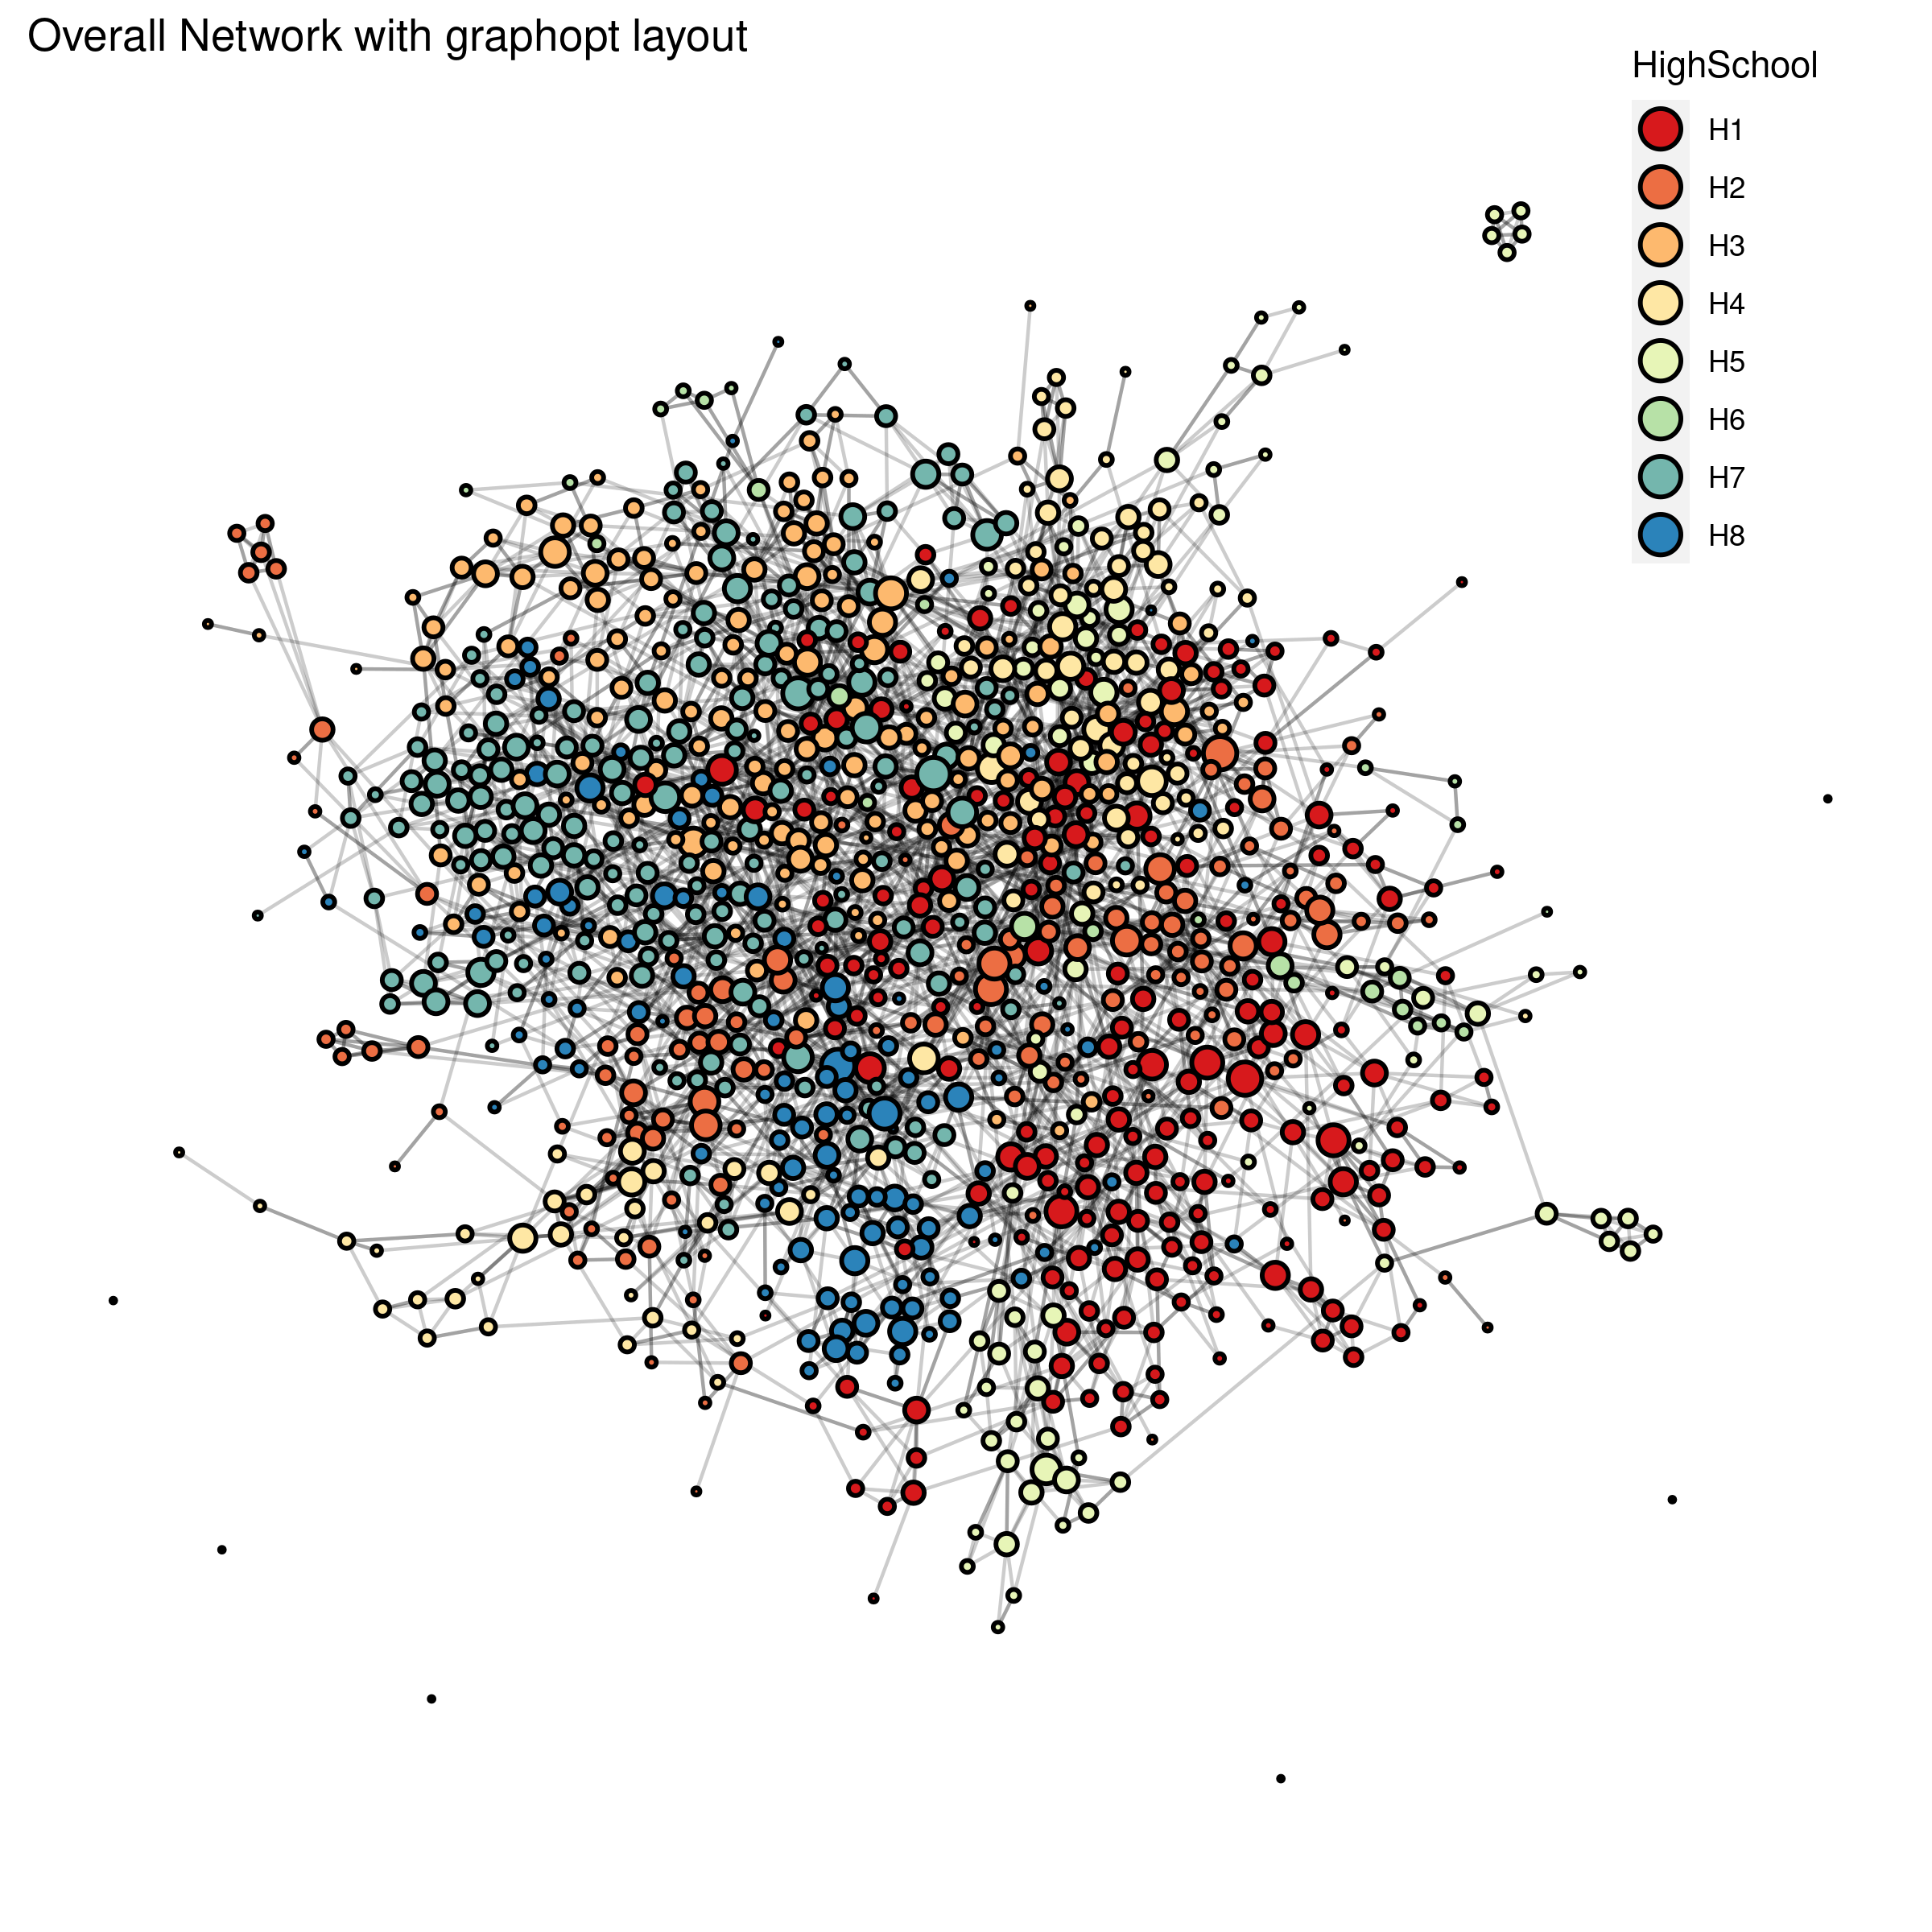
\includegraphics[width=0.7\linewidth]{figures/Networks/Layouts/Graph_OverallNetwork_with_no_highlight_graphopt_HighSchool___graphopt.png} 
        \caption{Overall network with a graphopt layout \cite{gabor2023}. Graphopt (graph optimization) uses physical analogies for defining attracting and repelling forces among the vertices and then the physical system is simulated until it reaches an equilibrium. It aimed to minimize the number of edge crossings to avoid visual cluttering, but in our case, we have too many edges everywhere and an emerging pattern is not clear.}
        \label{figure:networksLayoutsGRAPHOPT}
    \end{figure}

    \newpage

\subsubsection{Kamada-Kawai}

    \begin{figure}[h!]
        \centering
            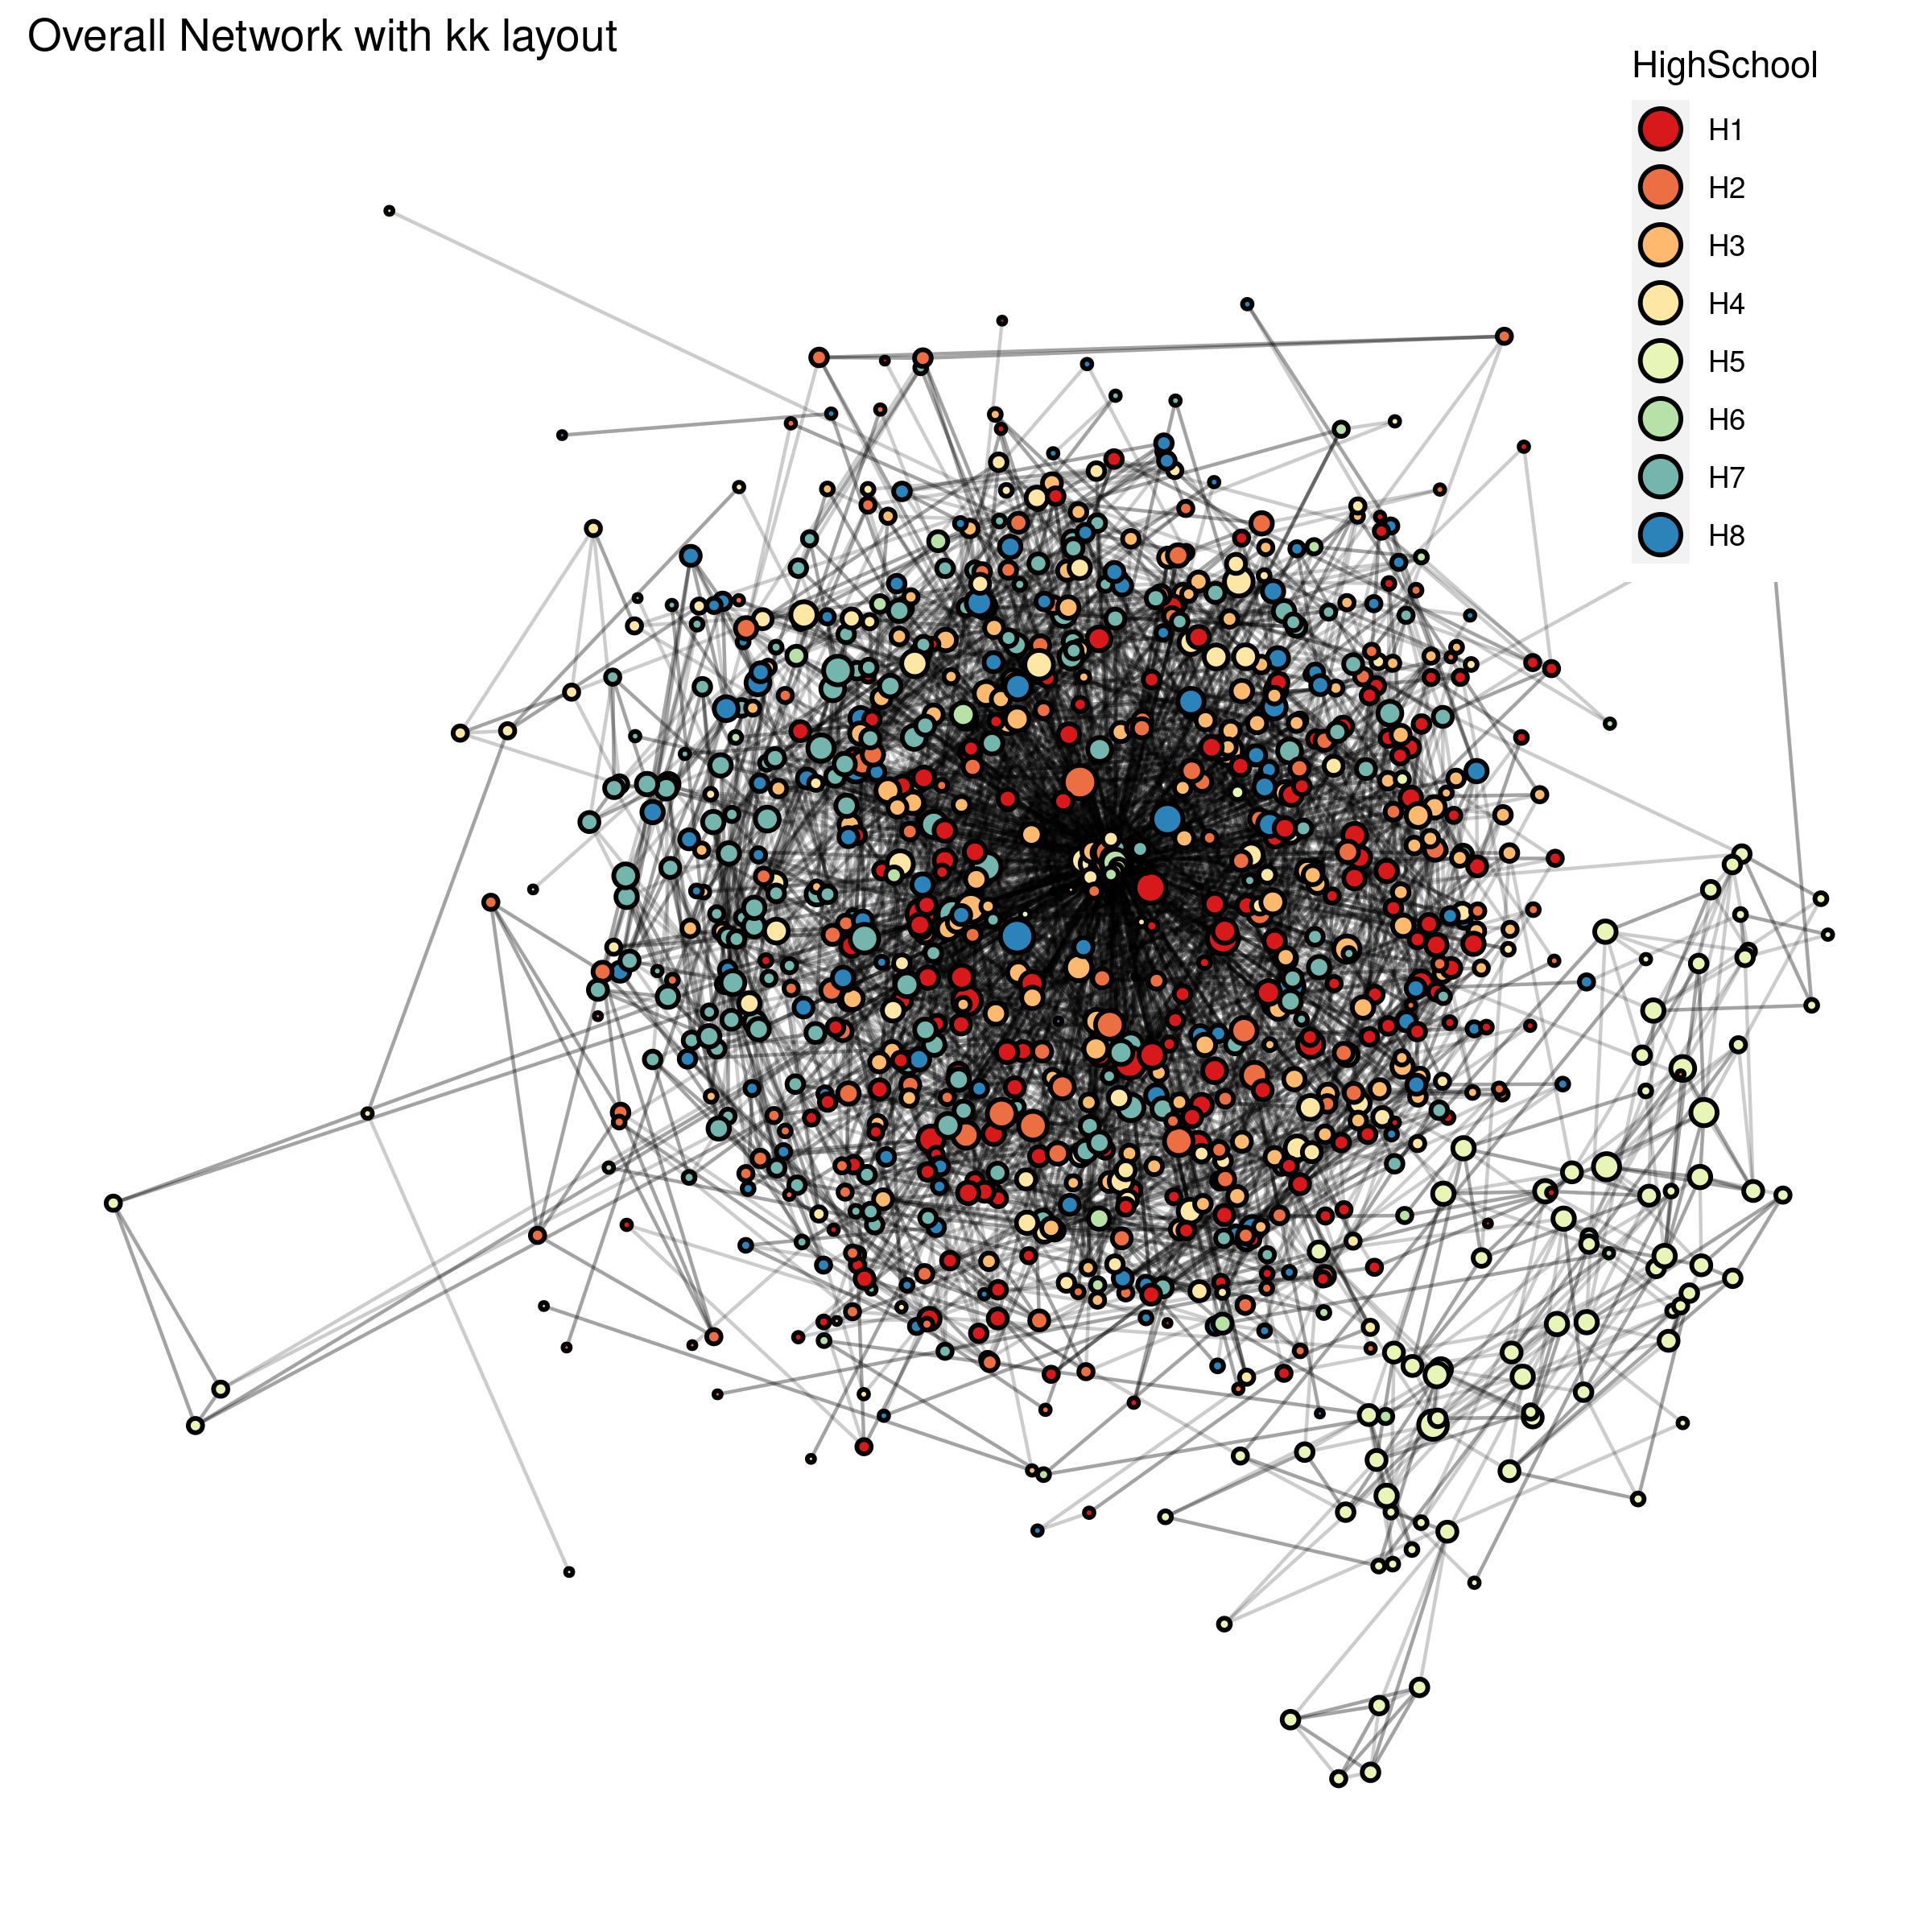
\includegraphics[width=0.7\linewidth]{figures/Networks/Layouts/Graph_OverallNetwork_with_no_highlight_kk_HighSchool___kk.png} 
        \caption{Overall network with a Kamada-Kawai algorithm \cite{Kamada1989}. It put emphasis on the distance as information. Here we see that more isolated nodes are on the outside, and more dense connected areas in the middle. Very useful in other contexts, but again not an ideal choice for us as the core of the network is just a mess of black lines.}
        \label{figure:networksLayoutsKK}
    \end{figure}    

    \newpage

\subsubsection{MDS}

    \begin{figure}[h!]
        \centering
            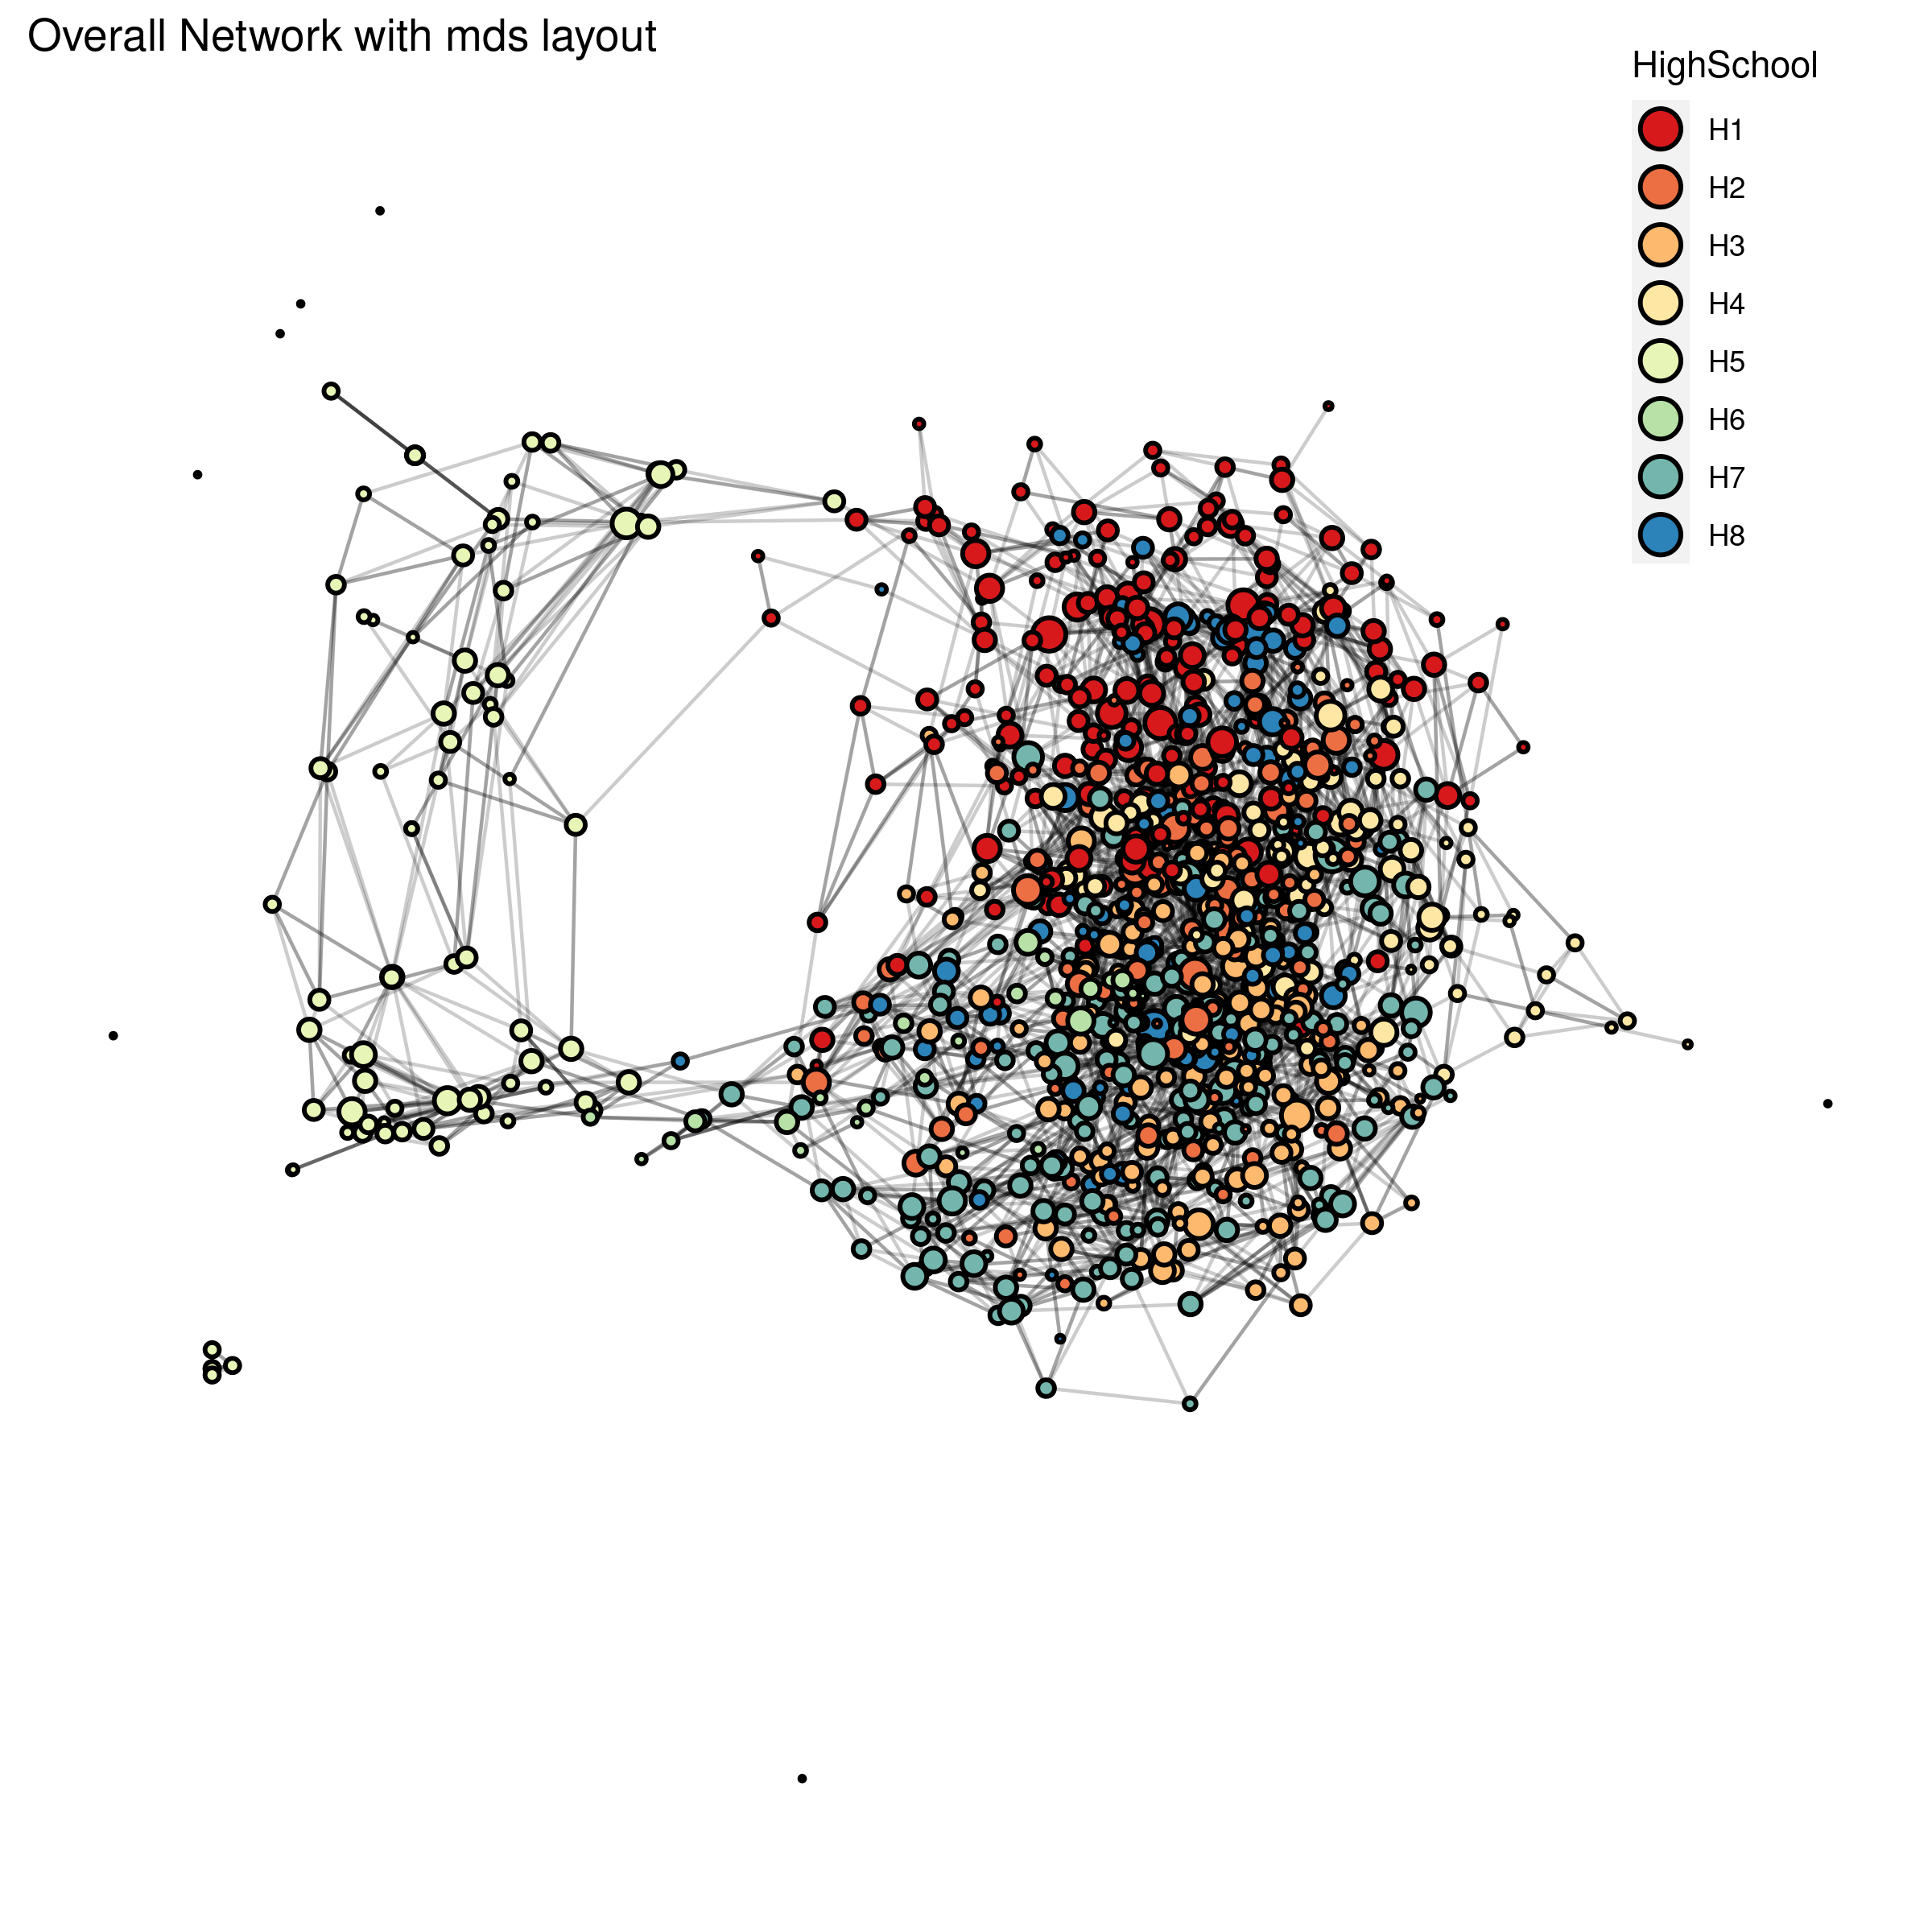
\includegraphics[width=0.7\linewidth]{figures/Networks/Layouts/Graph_OverallNetwork_with_no_highlight_mds_HighSchool___mds.png} 
        \caption{Overall network with \gls{mds} \cite{Buja2008}. When the dissimilarities are distances between high-dimensional objects, MDS acts as a dimension reduction technique. When the dissimilarities are the shortest-path distances in a graph, MDS acts as a graph layout technique. This is our preferred default method because it balances clusters groups of friends together which have some common attributes}
        \label{figure:networksLayoutsMDS}
    \end{figure}    

% MDS Original reference with no DOI http://www.stat.yale.edu/~lc436/papers/JCGS-mds.pdf

    \newpage

\subsubsection{Grouping}

    \begin{figure}[h!]
        \centering
            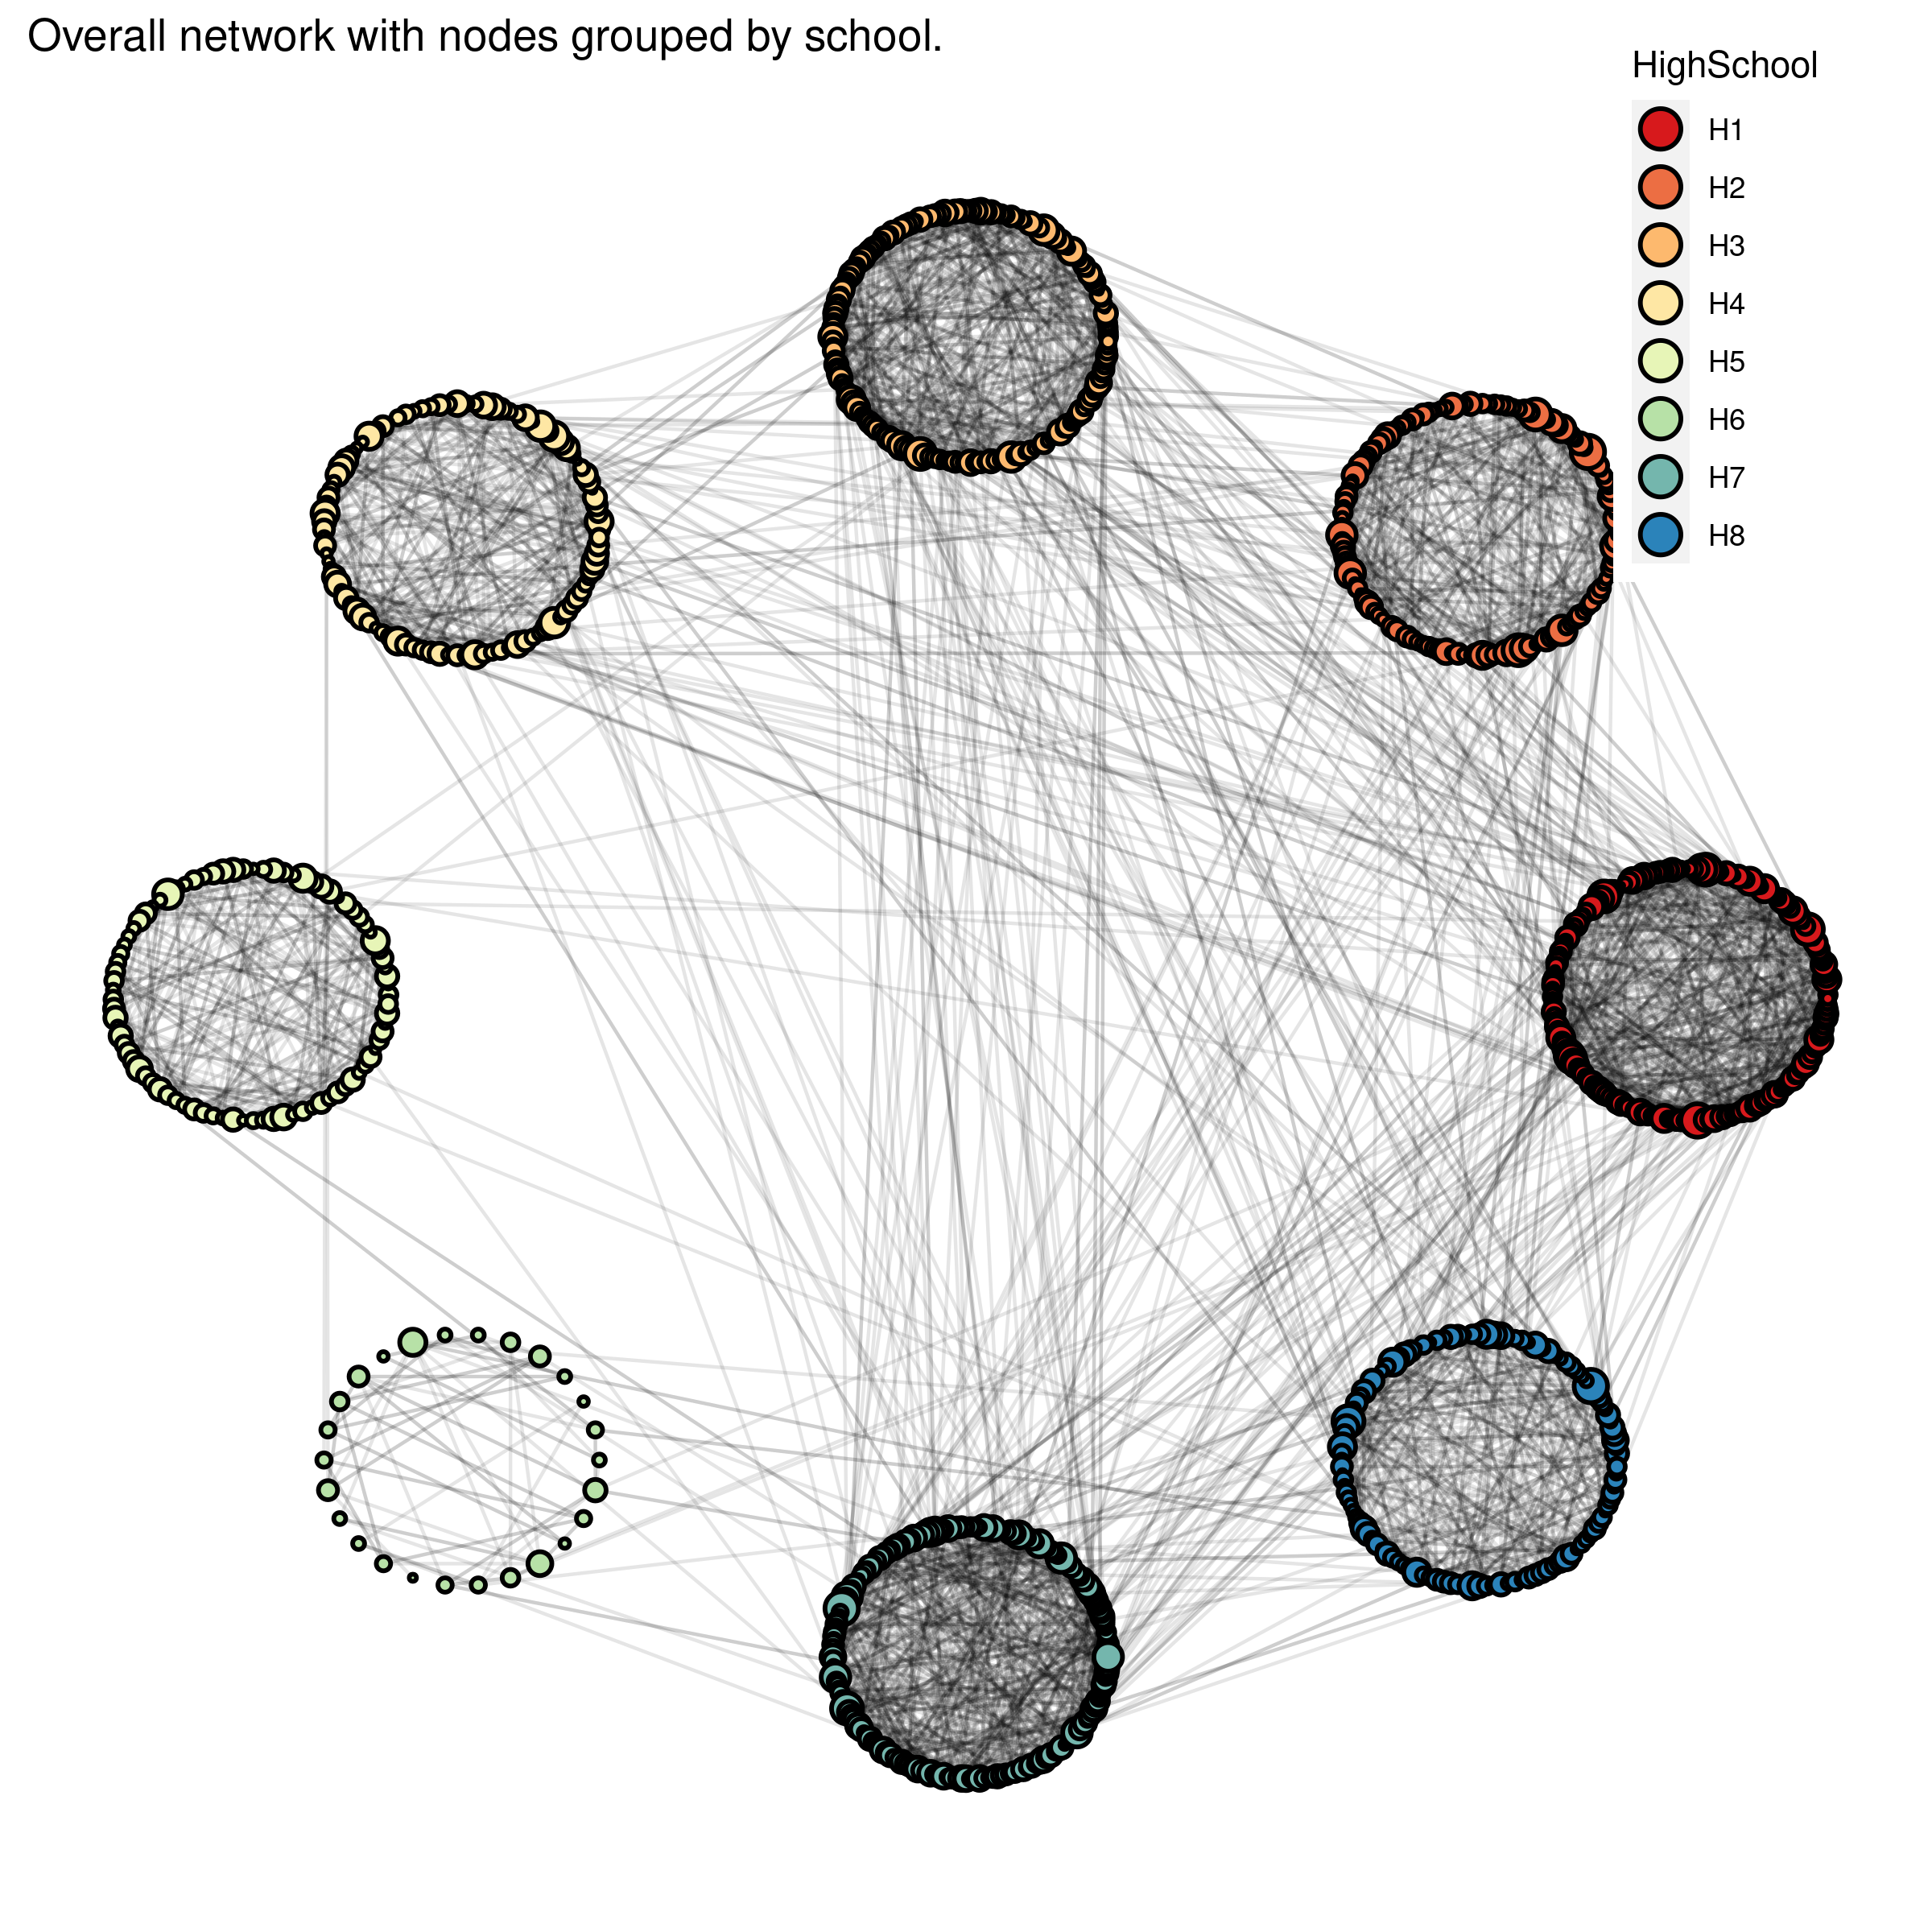
\includegraphics[width=0.7\linewidth]{figures/Networks/Layouts/Graph_OverallNetwork_HS_societal_HighSchool___manual.png} 
        \caption{Overall network sorting nodes into circles, where each circle is a high school. Here is hard to see relationships inside high schools since are densely connected, but ok to see the proportion of relationships between every two pairs of high schools.}
        \label{figure:networksLayoutsMANUAL}
    \end{figure}        

    \newpage

\subsubsection{Geographical}

    \begin{figure}[h!]
        \centering
            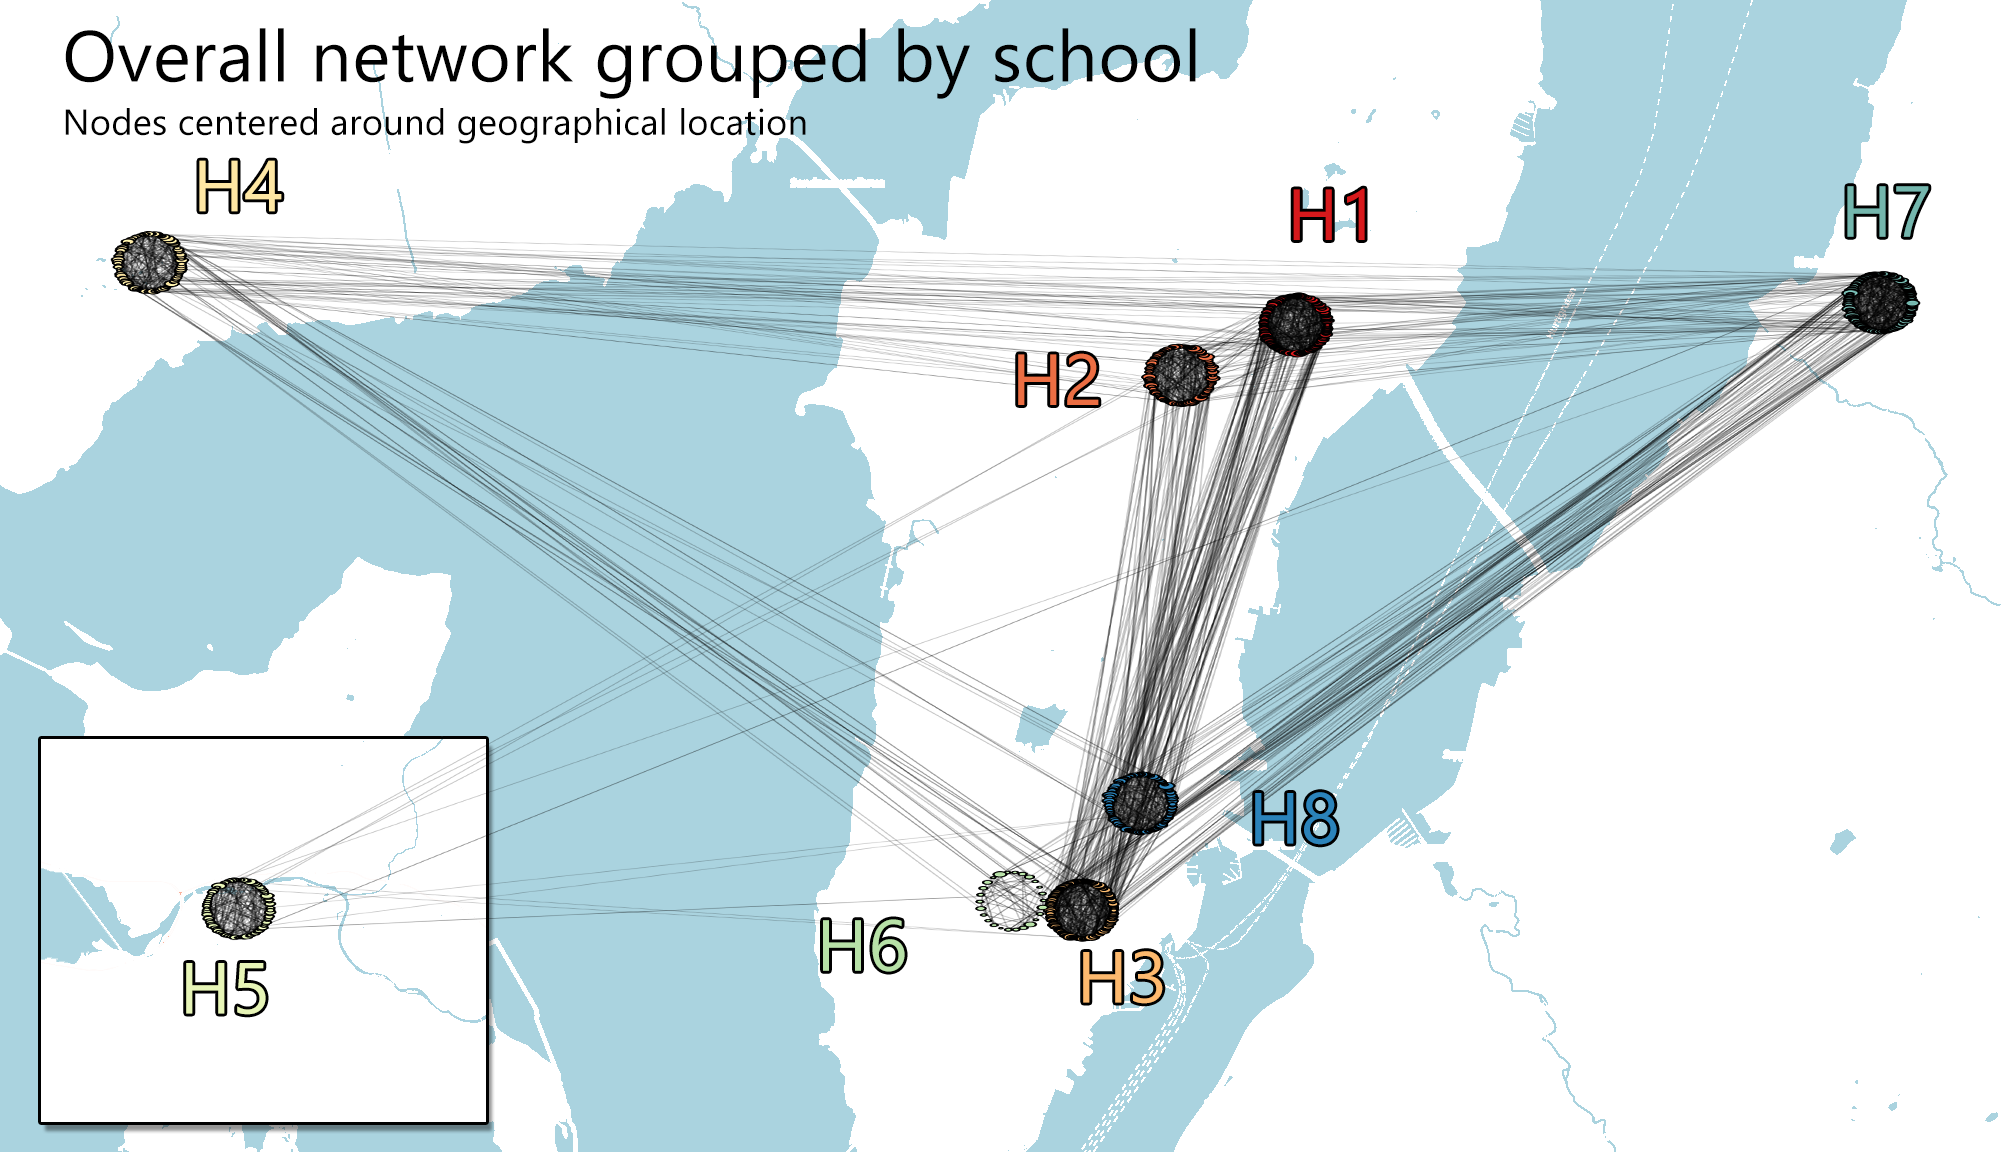
\includegraphics[width=0.9\linewidth]{figures/Networks/Layouts/schoolmapsGraph.png} 
        \caption{Overall network sorting nodes into circles placed according to high-school geographical location. A background outlined map of Tromsø from OpenStreetMaps has been added. Note that H5 is about 120km away from the rest and is brought closer for better visualization.}
        \label{figure:networksLayoutsGEOGRAPHICAL}
    \end{figure}        

    \newpage

\section{Networks metrics}

\subsection{How important is a node in a network?}

% Centralities, correct terminology! https://eehh-stanford.github.io/SNA-workshop/graphs.html#dyads-triads-and-other-local-structures

Nodes are not only important because they have many connections as we saw in section \ref{network:Connectivity}. The following metrics can help you identify nodes in the network that might also be relevant. But none of them is a better or worse method, it depends on what you consider to be important in your context:

\subsubsection{Degree centrality}

The most obvious one is to measure the number of connections \cite{Freeman1978}. In social networks, well-connected nodes are people with high popularity, which tends to be indicative of importance. In medical interventions, we like to target high connectivity nodes to become healthy because they tend to influence their peers to become healthy as well. In figure \ref{figure:networksLayoutsMDS} we can see the network with the node size proportional to the number of connections each student has.

\subsubsection{Closeness centrality}

In this context, we measure the importance of the nodes proportionally to their path with any other given node \cite{Freeman1978}. The idea is that an important node is one that is capable of reaching other nodes very quickly. The importance of this is more obvious in topology networks with weighted edges, where a town can be well connected to other towns, but using semi-destroyed and badly maintained roads, making it a less attractive node to put a central hub. In comparison, a town that is less connected but with a newly built 4 lanes highway, might be a better option. When a closeness centrality number is high, it means that the node is central in the network and is close to other nodes in the network. This indicates that the node has better accessibility to other nodes and can easily reach these nodes. An example of this metric can be seen in figure \ref{figure:networksCloseness}.

    \begin{figure}[h!]
        \centering
            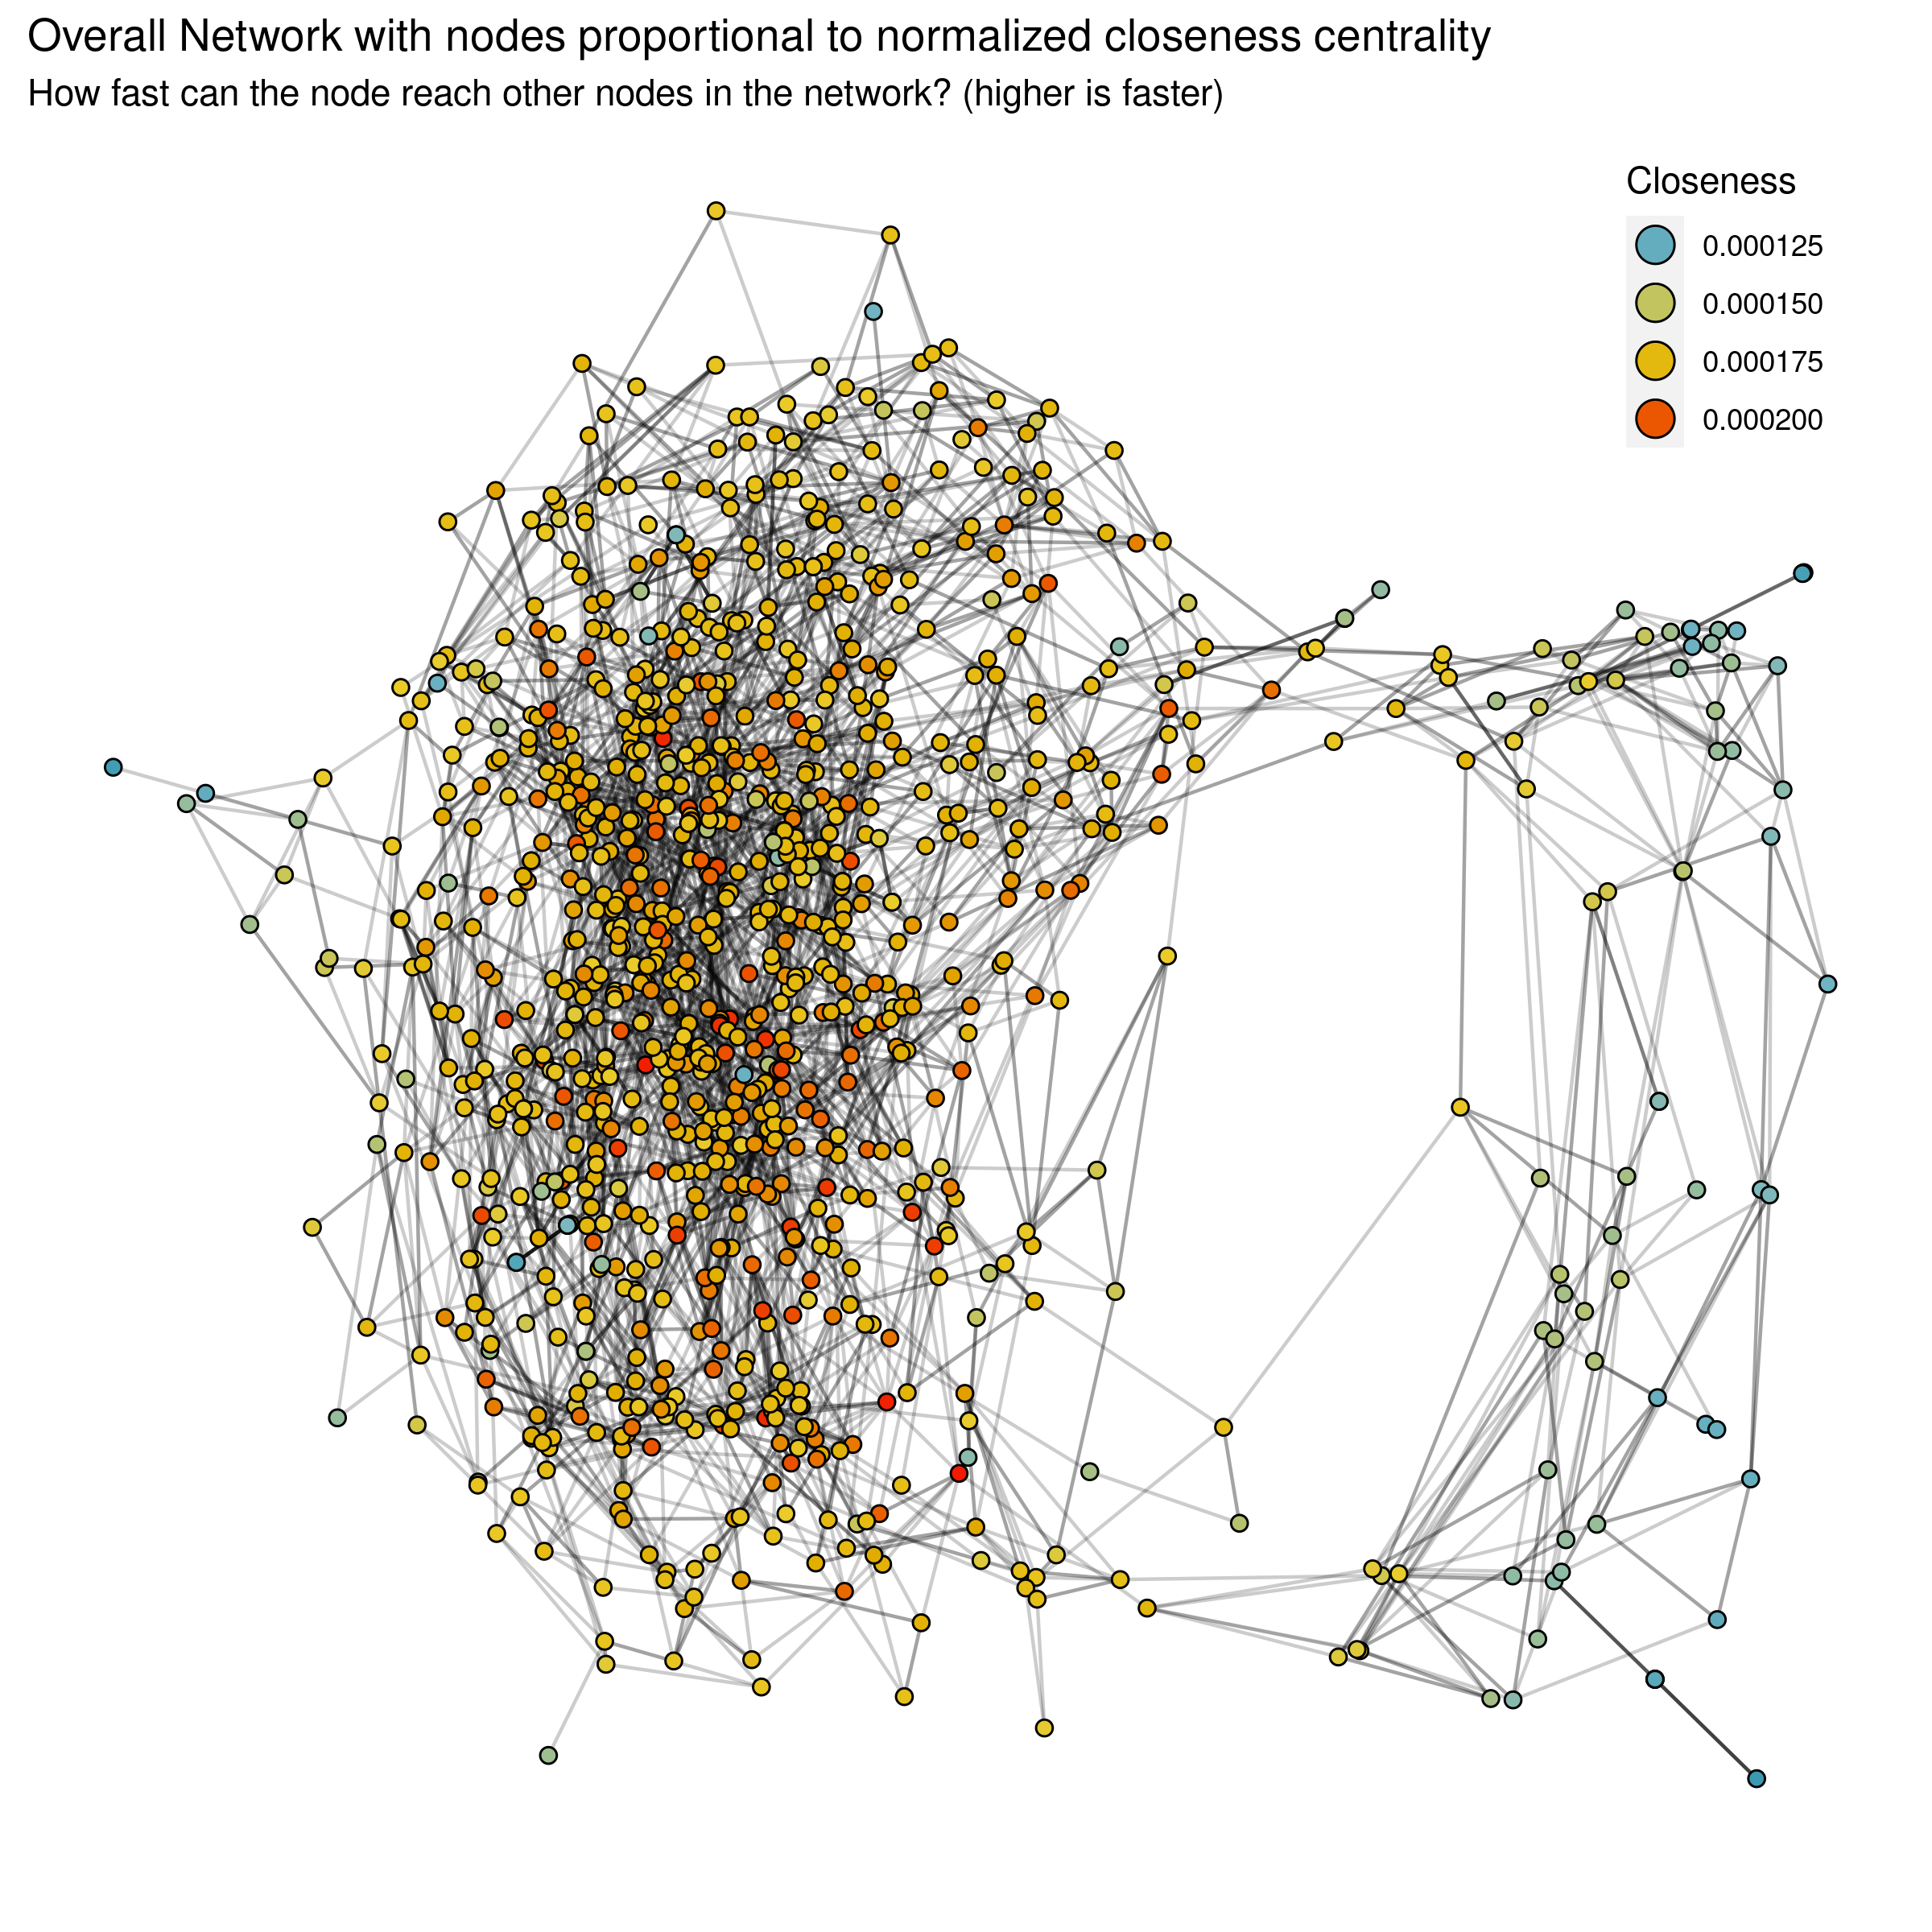
\includegraphics[width=0.9\linewidth]{figures/Networks/Centralities/Graph_temporalEdgesDF_centralitiesDF_Closeness___mds.png} 
        \caption{Overall network coloring nodes by their closeness. Disconnected nodes and subnetworks have outlier values and have been removed for better color scale}
        \label{figure:networksCloseness}
    \end{figure}      

\subsubsection{Betweenness centrality}

Central nodes are nodes that connect several subnetworks together \cite{Freeman1978}. In epidemiology identifying these nodes are critical because we can stop the progress of the disease by targeting these nodes alone, and thus isolating each of the individual clusters. An example of this metric can be seen in figure \ref{figure:networksBetweenness}.

    \begin{figure}[h!]
        \centering
            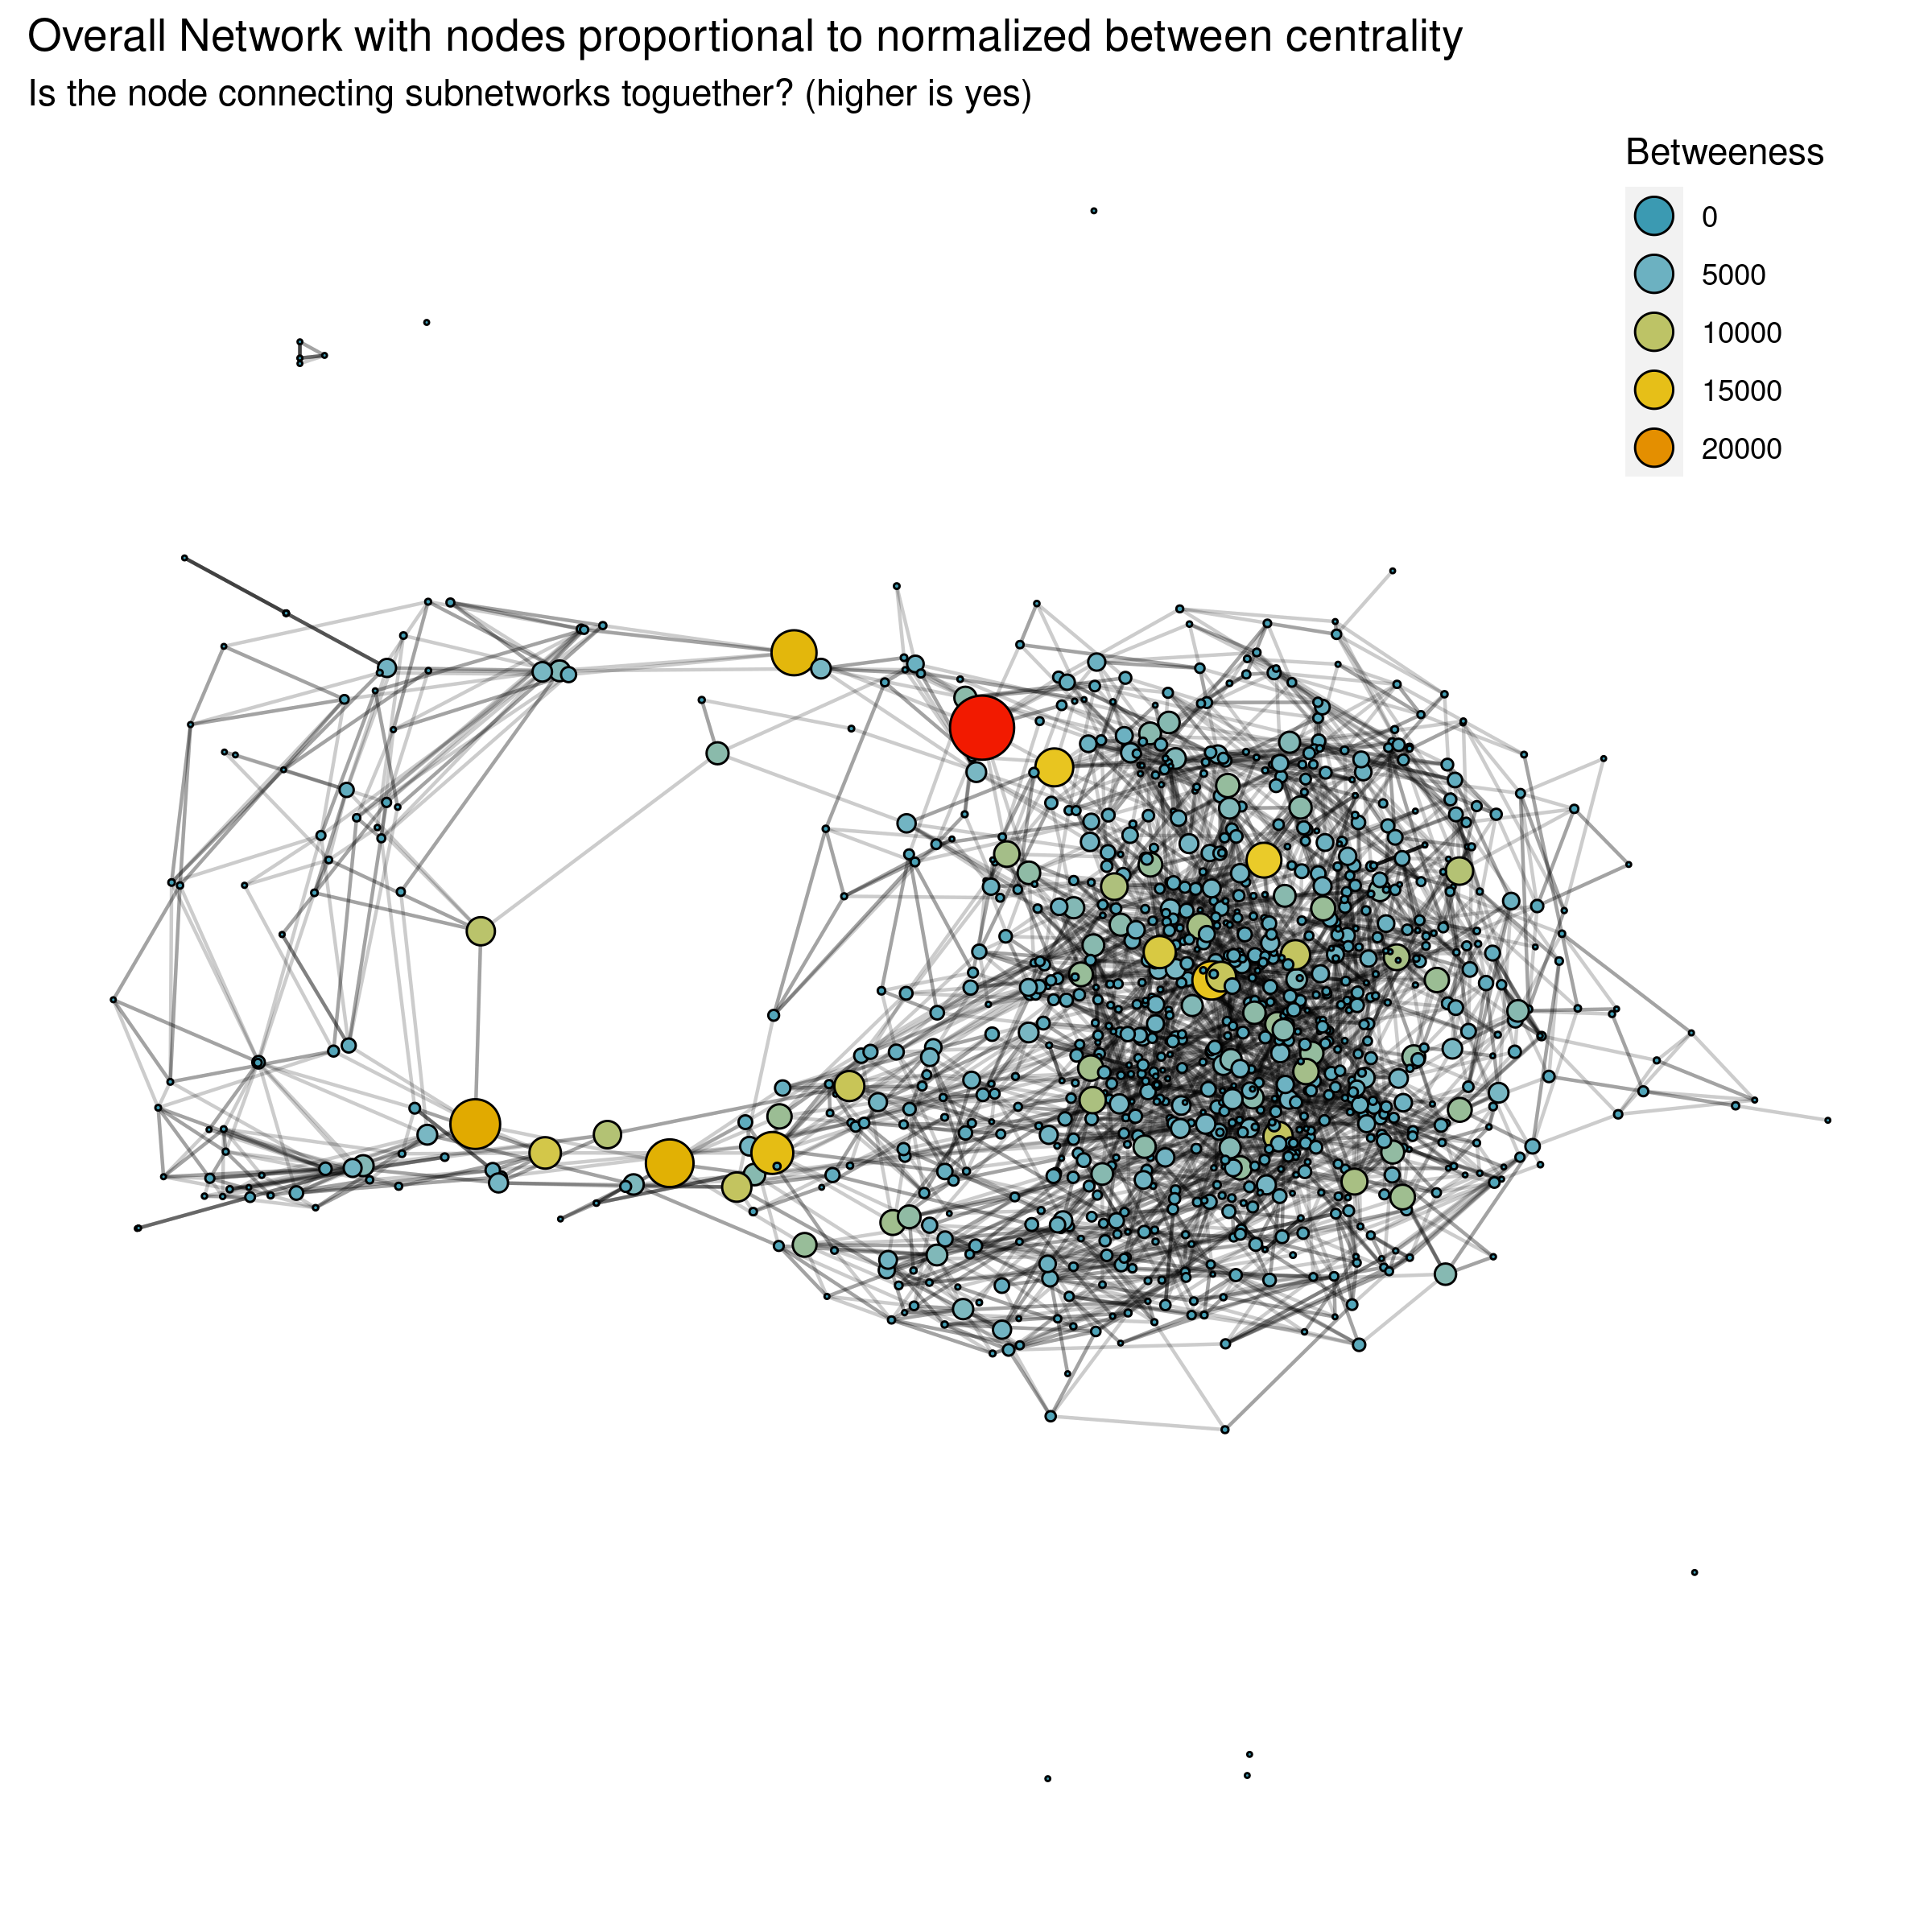
\includegraphics[width=0.9\linewidth]{figures/Networks/Centralities/Graph_overallEdgesDF_centralitiesDF_Betweeness___mds.png} 
        \caption{Overall network coloring nodes by their betweenness. Node size is proportional to betweenness.}
        \label{figure:networksBetweenness}
    \end{figure}      

\subsubsection{Eigencentrality}

When you don't care about the number of connections, but about the quality of the connections, then eigencentrality is what is used to measure the important nodes \cite{Bonacich1972}. In general, vertices with high eigenvector centralities are those which are connected to many other vertices which are, in turn, connected to many others, and so on. An example of this metric can be seen in figure \ref{figure:networksEigen}.

    \begin{figure}[h!]
        \centering
            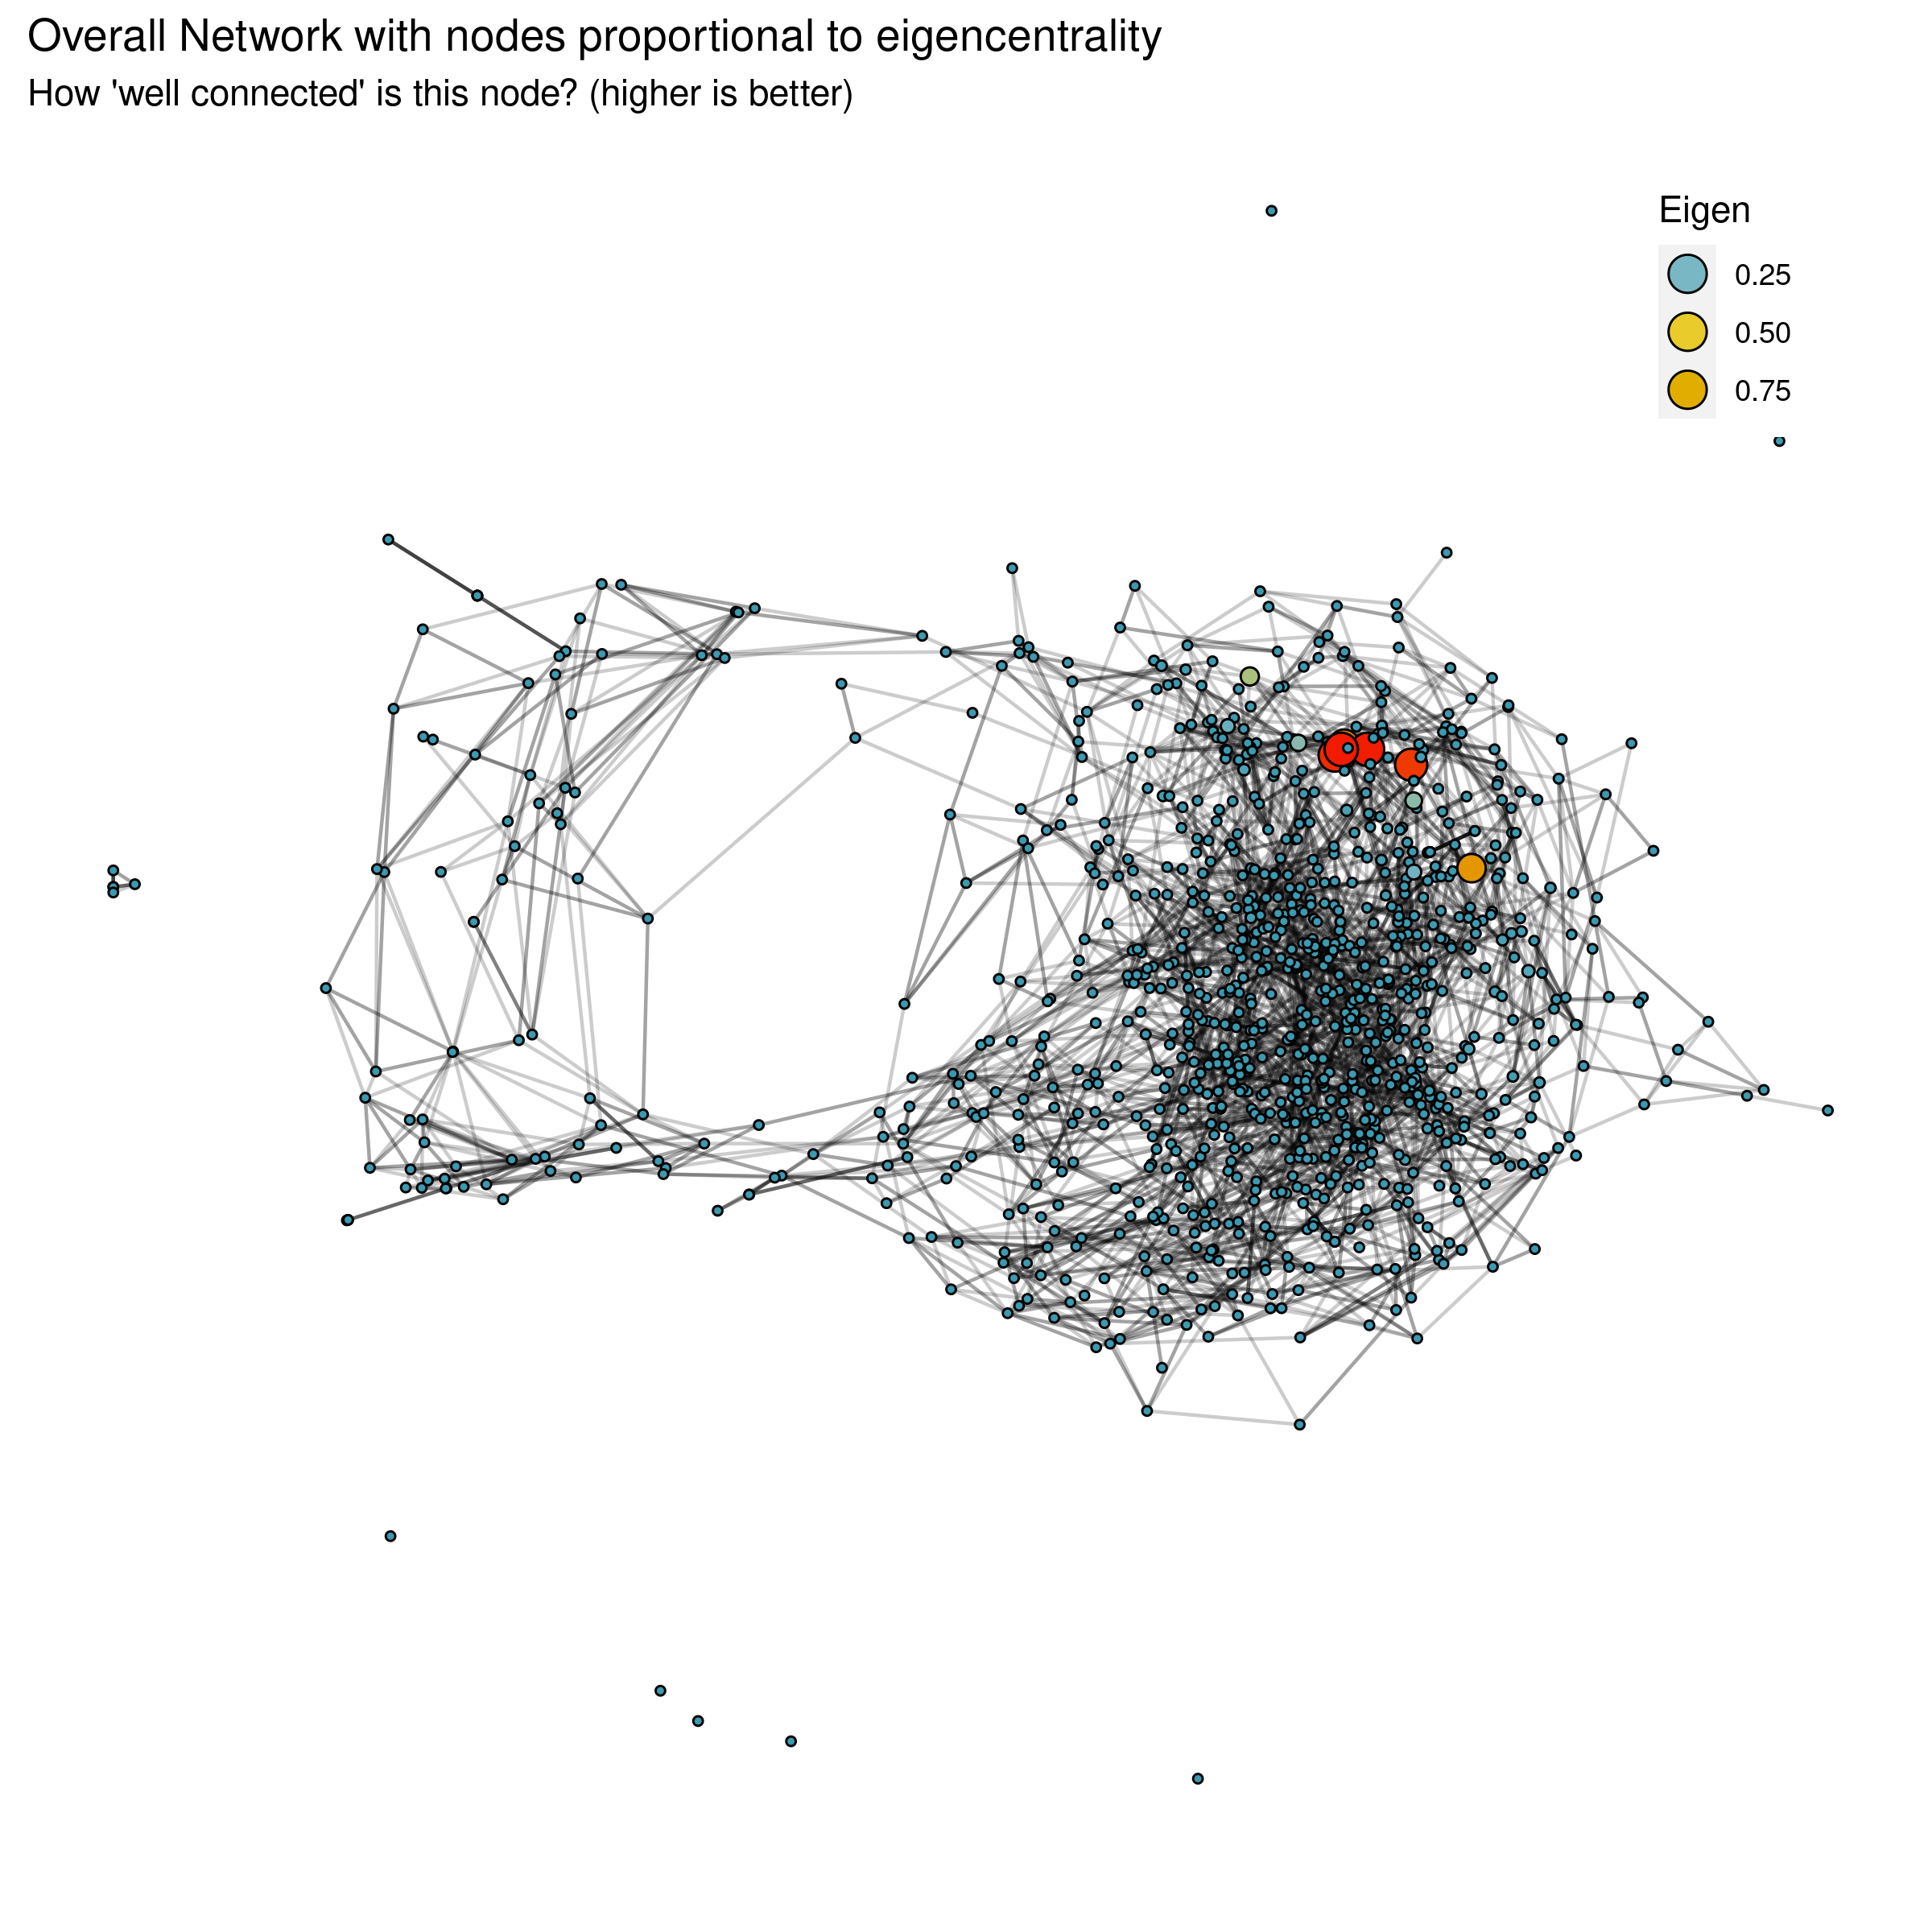
\includegraphics[width=0.9\linewidth]{figures/Networks/Centralities/Graph_overallEdgesDF_centralitiesDF_Eigen___mds.png} 
        \caption{Overall network coloring nodes by their eigencentrality. Node size is also proportional to eigencentrality. A few nodes are popular people also connecting to other popular people.}
        \label{figure:networksEigen}
    \end{figure}      

\subsubsection{Bonacich Centrality}
 
Is the same as Eigencentrality, but you get a decay factor the further away you are from well-connected people \cite{Bonacich1972}.

\subsection{Connectivity average}

Connectivity is the average chosen centrality per node in the network. It gives you an idea of how well the network is interconnected. Higher degree centrality numbers mean that information or diseases travel around much easier. In table \ref{table:networksHS} we can see that connectivity is not constant in the network, for example, some schools display higher connectivity than others, and the same goes for sex dynamics.

    \begin{figure}[h!]
        \centering
            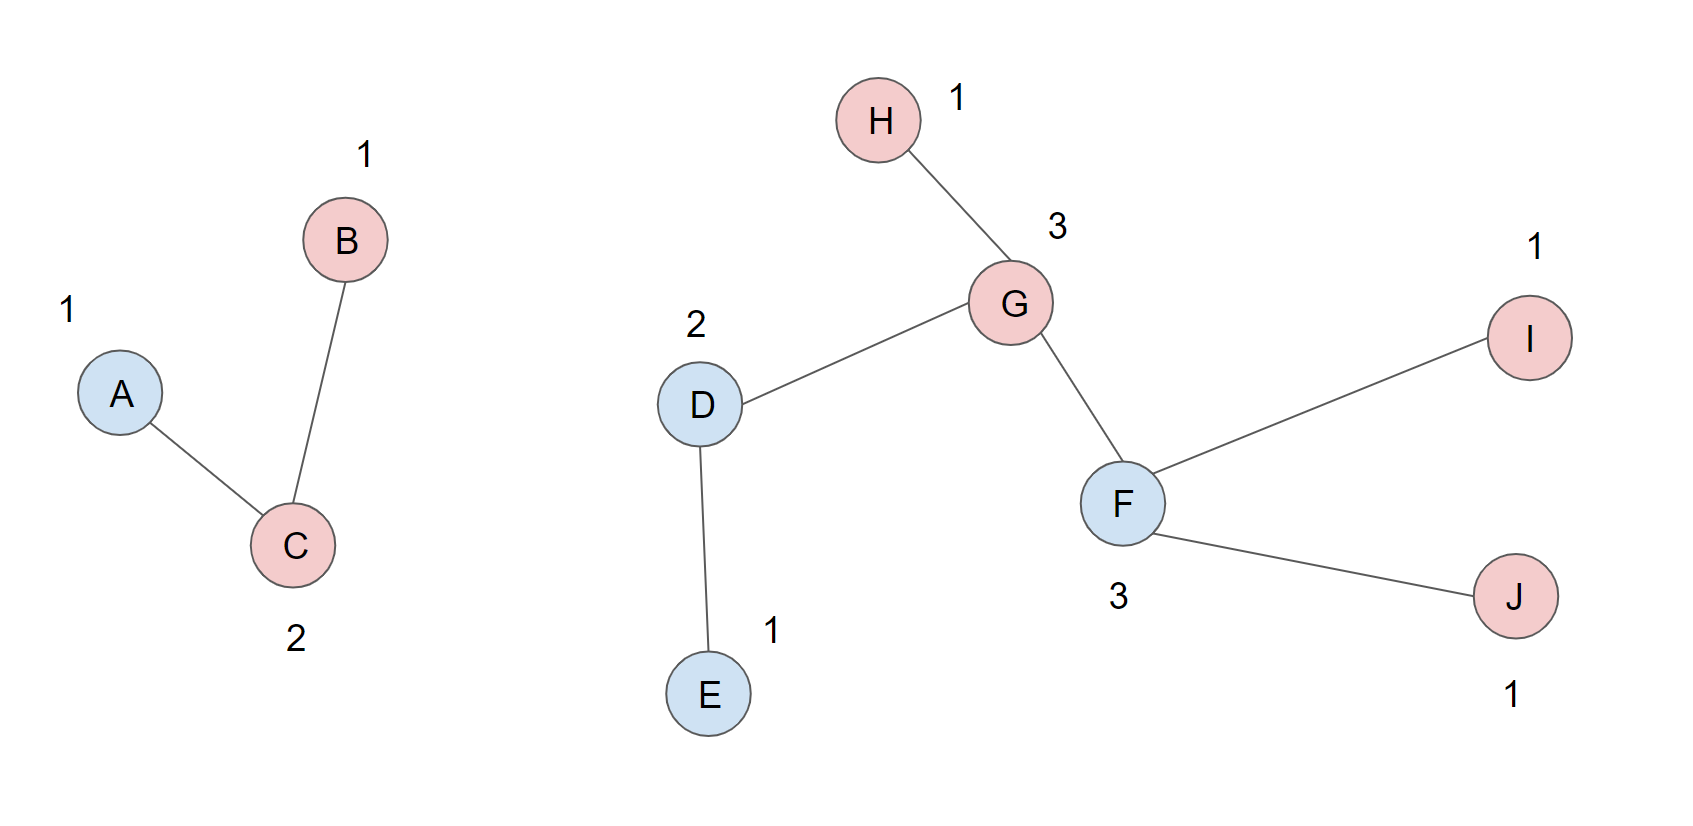
\includegraphics[width=0.7\linewidth]{figures/Networks/Concepts/edgesConnectivity.png} 
        \caption{A network with two components. Nodes are labeled with the number of degree centrality in each. On the left component, we have an average degree of 1.3, while in the right component, we have an average degree of 1.71}
        \label{figure:networksConnectivity}
    \end{figure}   

\label{figure:networksHS}
\begin{table}[h!]
    \centering
    \caption{The average centralities measures for the whole population, each high school, and also men and women. Notice that in H5 we have a higher amount of disconnected triads, which causes outliers in the average value for closeness.}
    \renewcommand{\arraystretch}{1.7}
    \begin{tabular}{rccccc|}
    \cline{2-6}
    \multicolumn{1}{l|}{}                                    & \multicolumn{1}{l}{\cellcolor[HTML]{FFFFC7}Degree} & \multicolumn{1}{l}{\cellcolor[HTML]{FFFFC7}Closeness} & \multicolumn{1}{l}{\cellcolor[HTML]{FFFFC7}Between} & \multicolumn{1}{l}{\cellcolor[HTML]{FFFFC7}Eigen} & \multicolumn{1}{l|}{\cellcolor[HTML]{FFFFC7}Bonacich} \\ \hline
    \multicolumn{1}{|l|}{\cellcolor[HTML]{FBDBB5}Population} & 5.34                                               & 0.0014                                                & 2362                                                & 0.0087                                            & -0.0215                                               \\ \hline
    \multicolumn{6}{|c|}{\cellcolor[HTML]{C0C0C0}High school}                                                                                                                                                                                                                                                                               \\ \hline
    \multicolumn{1}{|r|}{\cellcolor[HTML]{EFEFEF}H1}         & 5.4                                                & 0.0002                                                & 2696                                                & 0.0015                                            & -0.0155                                               \\
    \multicolumn{1}{|r|}{\cellcolor[HTML]{EFEFEF}H2}         & 5.06                                               & 0.0002                                                & 2197                                                & 0.0009                                            & 0.0084                                                \\
    \multicolumn{1}{|r|}{\cellcolor[HTML]{EFEFEF}H3}         & 5.51                                               & 0.0002                                                & 2501                                                & 0.0015                                            & -0.0423                                               \\
    \multicolumn{1}{|r|}{\cellcolor[HTML]{EFEFEF}H4}         & 5.44                                               & 0.0002                                                & 2033                                                & 0.0011                                            & -0.0154                                               \\
    \multicolumn{1}{|r|}{\cellcolor[HTML]{EFEFEF}H5}         & 4.95                                               & 0.0148                                                & 1913                                                & 0.0000                                            & 0.0689                                                \\
    \multicolumn{1}{|r|}{\cellcolor[HTML]{EFEFEF}H6}         & 4.23                                               & 0.0002                                                & 2258                                                & 0.0002                                            & -0.2174                                               \\
    \multicolumn{1}{|r|}{\cellcolor[HTML]{EFEFEF}H7}         & 5.76                                               & 0.0002                                                & 2526                                                & 0.0038                                            & 0.0294                                                \\
    \multicolumn{1}{|r|}{\cellcolor[HTML]{EFEFEF}H8}         & 5.1                                                & 0.0002                                                & 2132                                                & 0.0627                                            & -0.1456                                               \\ \hline
    \multicolumn{6}{|c|}{\cellcolor[HTML]{BCFBBB}Sex}                                                                                                                                                                                                                                                                                       \\ \hline
    \multicolumn{1}{|r|}{\cellcolor[HTML]{B7FDFA}Men}        & 5.31                                               & 0.0011                                                & 2405                                                & 0.0153                                            & -0.0106                                               \\
    \multicolumn{1}{|r|}{\cellcolor[HTML]{FFBED5}Women}      & 5.37                                               & 0.0017                                                & 2317                                                & 0.0019                                            & -0.0328                                               \\ \hline
    \end{tabular}
\end{table}


\subsection{Density}

Density is another overview of the number of relationships in a network. Is the amount of total connections divided by the amount of possible connections. Unlike connectivity, this value is bounded between 0 and 1. Density by itself is not an exciting metric and needs to be compared with another density to get some useful information. For example, we can compare the friendship density of the high schools in Northern Norway, with the density in Southern Norway to see if there is a significant difference. We can do the same for nodes inside a network, such as comparing the friendship density of men against the friendship density of women.

    \begin{figure}[h!]
        \centering
            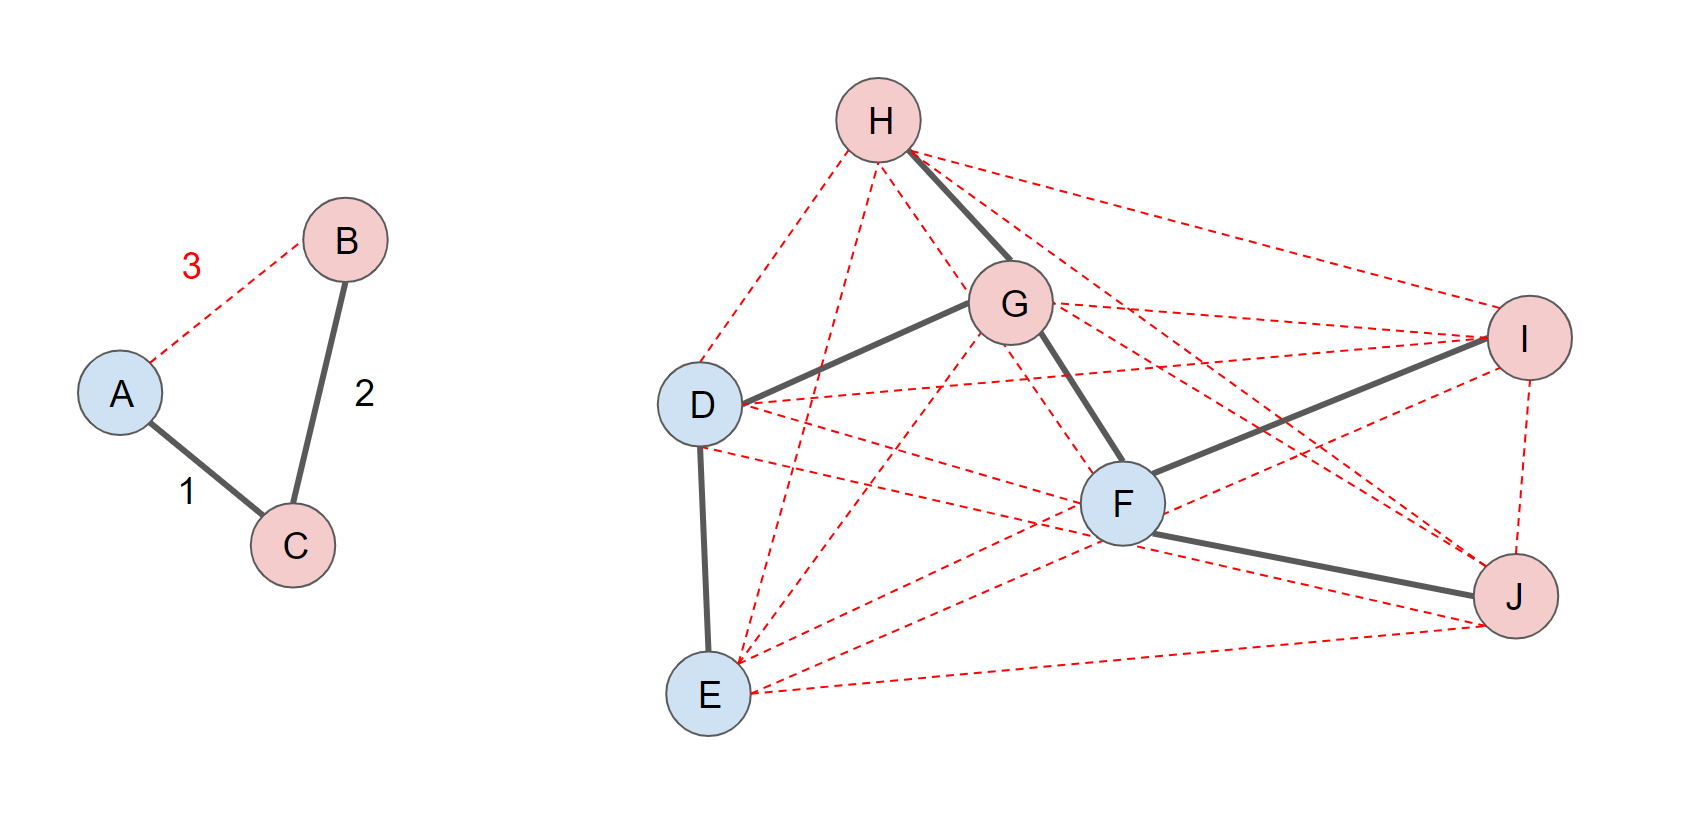
\includegraphics[width=0.7\linewidth]{figures/Networks/Concepts/edgesDensity.png} 
        \caption{A network with two components. Black edges thick represent existing edges, and red thin and dashed edges represent possible edges. On the left component, the 3 possible edges are shown and labeled. On the right component, no edge is labeled. The left component has a density of 2/3 (66\%), while the right component has a density of 6/49 (12\%). Notice that the right component, despise having higher average connectivity, also has a lower density.}
        \label{figure:networksDensity}
    \end{figure}    


\subsection{Homophily}
\label{network:homophily}

Homophily is the core reason why social network studies work. Individuals tend to form strong bonds with people who are similar to them by factors such as marital status, race, economics, nationality, common interests, and many more \cite{Stehl2013, Moody2001, Qian2007, Cheadle2012, McPherson1987, Sergio2009, Kossinets2009, McPherson2001, Smith2014, Karimi2018, Lee2019, Avin2020, Asikainen2020}. This is also the biggest challenge when interpreting data, as we cannot be sure if individuals who are close to each other are influencing each other, or if they are simply sharing an environmental factor that influences everyone at the same time to no fault of the nature of their relationships.

Homophily is the ratio of, nodes that have an edge to another node that has the same property, against nodes that have an edge to a node of different property. Density only cares that there's an edge, while homophily cares about what types of nodes are being connected. Similar to density, homophily needs to be compared to another homophily number to gain some useful information.

First, we define edges that connect two nodes with the same attributes:
    \begin{equation}
        H_{any} \subseteq  \left\{ (x,y) | (x,y) \in V^2  \land x \neq y  \land x_i = y_i \right\}
    \end{equation}
Second, we define edges that connect two nodes with the same given attribute:
    \begin{equation}
        H_{given} \subseteq  \left\{ (x,y) | (x,y) \in V^2  \land x \neq y  \land x_i = y_i = A \right\}      
    \end{equation}
Finally, we define edges that connect two nodes with either of them having a GIVEN attribute:
    \begin{equation}
        H_{either} \subseteq  \left\{ (x,y) | (x,y) \in V^2   \land  x \neq y \land  x_i = A | y_i = A \right\}
    \end{equation}    
For a given variable, there are two ways to calculate homophily:
    \begin{equation}
        Homophily_i =  \frac{|H_{any}|}{|E|}
    \end{equation}
    \begin{equation}
        Homophily_{i=A} =  \frac{|H_{given}|}{|H_{either}|}      
    \end{equation}
In figure \ref{figure:networkExampleWeights}, we have 9 edges. Edges \{B,C\} and \{H,G\} connect red to red. Edges \{A,D\} and \{D,E\} connect blue to blue. Therefore, we have 4 edges connecting the same colors out of 9 possible. $Homophily_{color} = 44.4\%$ . Specifically for red, we have the same edges \{B,C\} and \{H,G\} connecting red to red, and edges \{A,C\}, \{B,C\}, \{D,G\}, \{H,G\}, \{G,F\}, \{F,I\} and \{F,J\} connecting at least one red. Then, $Homophily_{color = red} = 28.6\%$.

Is also possible to do a binomial test on the homophily to check if it is significant. This is simply measuring how many nodes of the same attributes we have, and how many are friends between them. If the number of edges is proportional to the number of nodes, that indicates that the number of relationships within the same group is what we would expect by random chance. But if we have too little, or too many relationships among them, it might indicate that the group is biased toward forming relationships among themselves or avoiding each other. Following the figure \ref{figure:networkExampleWeights} example:

    \begin{itemize}
        \item How many edges are reds friending red? 2
        \item How many reds do we have? 6
        \item What is the probability of being red? 0.6 
    \end{itemize}

The calculated binomial test is:
    \begin{equation*}
         \dbinom{6}{2} \cdot 0.6^2 \cdot (1-0.6)^{6-2} = 0.14
    \end{equation*}
The probability $Homophily_{color = red} = 0.286$ is greater than we would expect by chance (0.14), however, is not greater by much. The p-value for a two-sided test is 0.23 indicating that we can't really tell if the reds are biased in this graph.

\subsection{Average path length}

For fully connected networks, the \gls{apl} is the average of all possible paths. If a network is not fully connected, then the average path length is infinite. In such cases is more interesting to find the APL per sub-network. \gls{apl} is related to density. Forming 4 different interesting cases:

\begin{itemize}
    \item  Low \gls{apl} and low density will have a close solution to a minimum spanning tree. This is a subset of edges that connects all the nodes without cycles and with the minimum possible edges or edge weight. This case is important because it shows the cheapest way to lay down roads connecting cities so all cities are connected, expending the least amount of money possible.
    \item  High \gls{apl} and low density mean all the nodes are connecting using very few edges. This is bad if we describe for example a network of roads, because it will have very long paths and at the same time all cars need to pass through the same common edges. This is good if we have an infectious disease because it means we can cut the network in half easily and avoid propagation.
    \item  Low \gls{apl} and high density. This case means that all the nodes are very well connected, and traveling from one to another is easy. As opposed to before, great for roads due to low traffic, but bad for diseases because is very difficult to slow down or stop the spread.
    \item  High \gls{apl} and high density. This means that you have many sub-networks that are very well connected, but the connection between sub-networks is done with a really low number of edges forming choking points.
\end{itemize}

\subsection{Coverage}

Coverage of a node refers to how many nodes you can reach from that particular node in equal or less a particular path distance. This is also referred to as how many steps you need to reach any given pair of nodes if their distances are all equal.

    \begin{figure}[h!]
        \centering
            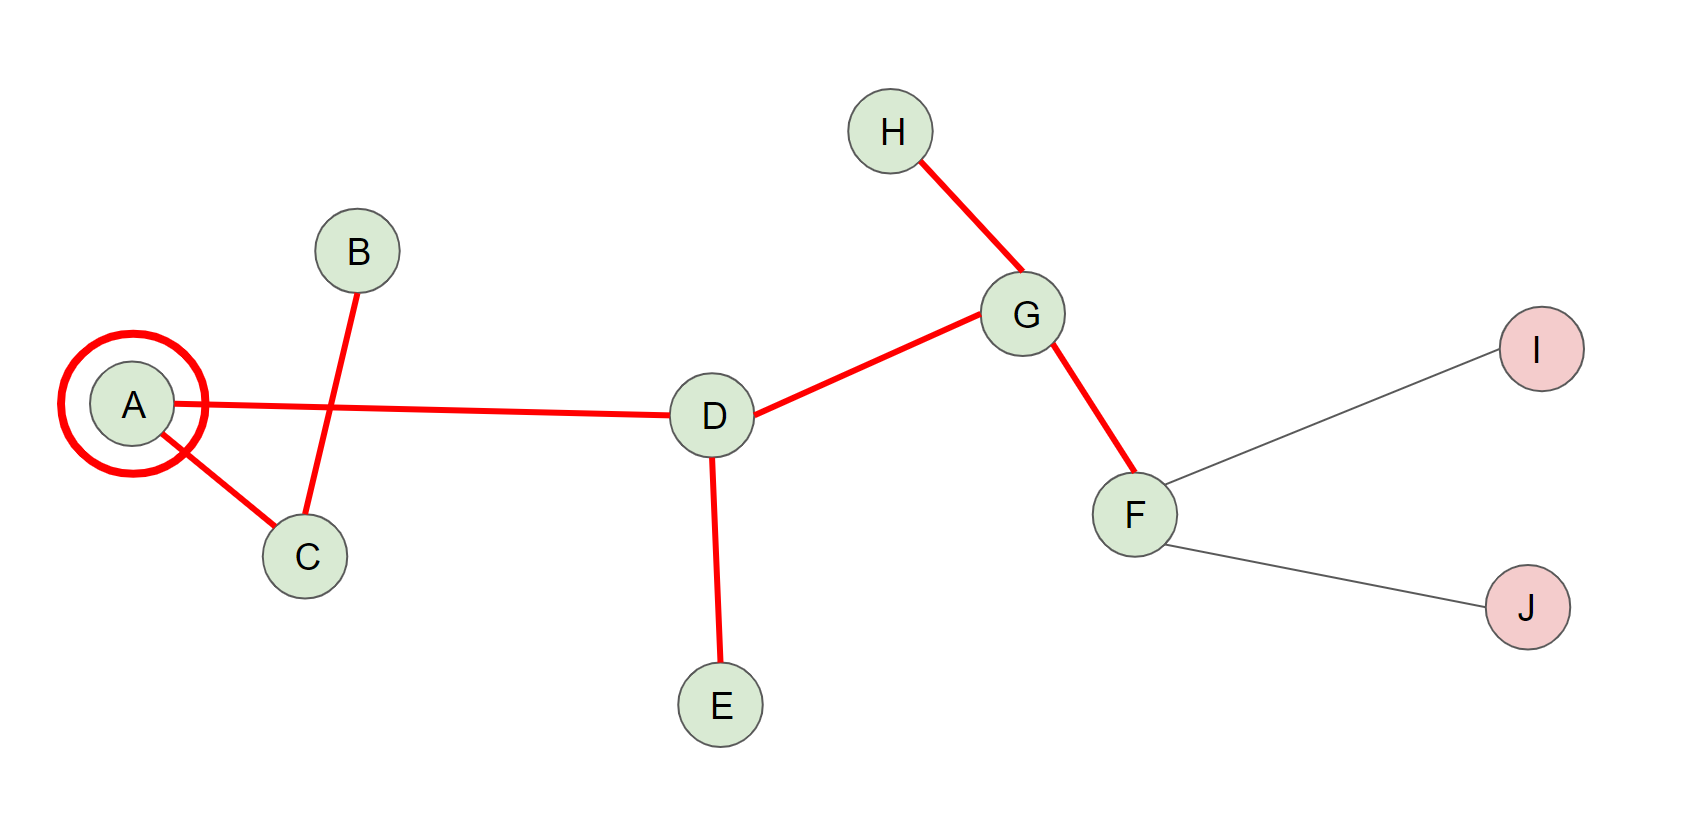
\includegraphics[width=0.7\linewidth]{figures/Networks/Concepts/coverage.png} 
        \caption{An example of coverage. For a given path of distance equal to 3, node A can reach all the green highlighted nodes using the red highlighted paths.}
        \label{figure:networkCoverage}
    \end{figure}

\subsection{Reachability}

Reachability refers to the average coverage per step in a network. Reachability is related to connectivity, as the network is more and more dense, is more easy to cover more nodes with fewer steps. This is an important variable when we deal with infectious diseases, if a large area of the network is reachable very quickly, the disease will spread very quickly as well.

    \begin{figure}[h!]
        \centering
            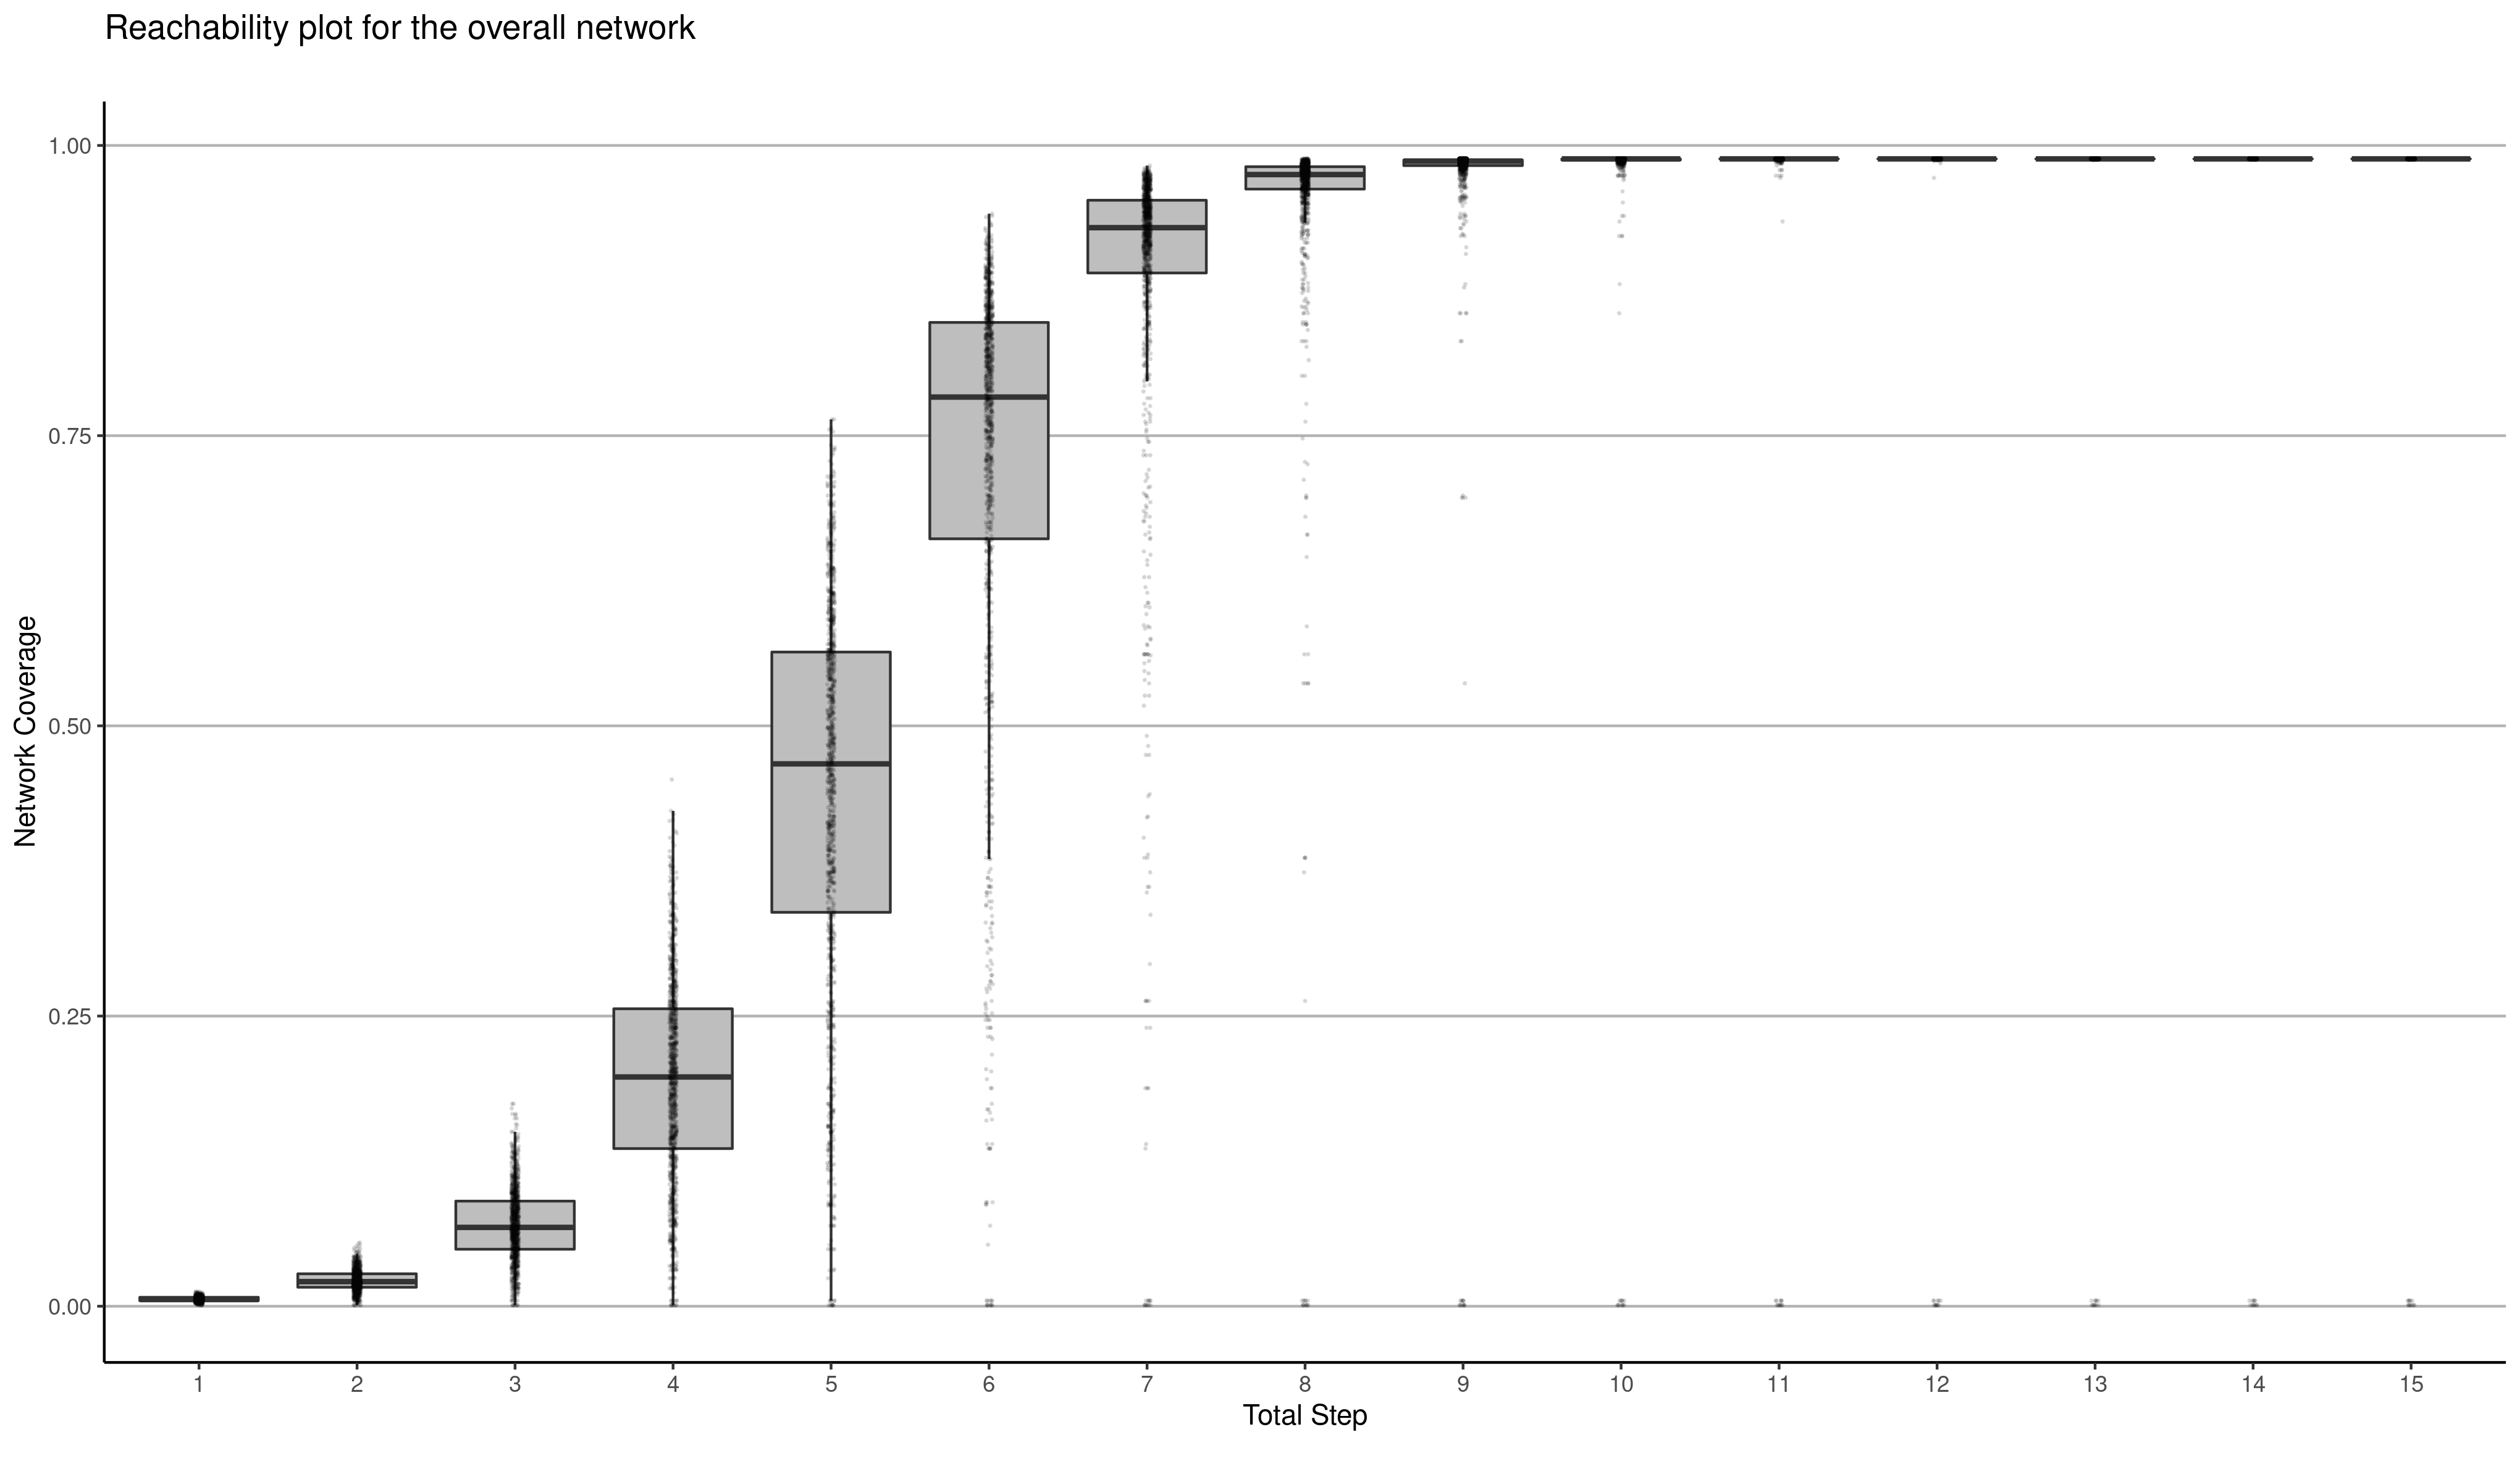
\includegraphics[width=0.7\linewidth]{figures/Networks/Reach/CategoricalBoxplot_reachplot_variable_value.png} 
        \caption{A reachability plot in the overall network. The x-axis represents the number of steps taken. The y-axis represents the proportion of network coverage. After 4 steps, we see that about 25\% of the nodes manage to cover 25\% of the network. In the next step, nearly 50\% of the nodes, cover 50\% of the network. In the next step, we see that the median surpasses the 75\% coverage, so the nodes reach grows exponentially in this network. It never reaches 100\% because some of the nodes are isolated, we see this better in the outliers that start showing from step 7 at the bottom of each box.}
        \label{figure:networksReach}
    \end{figure}    

\subsection{Simulations}

Finally, let's talk about how all these concepts can be put together in a practical case, which is how a disease can advance through the network. This topic has already been studied, to the point that even a zombie apocalypse has been described and published. \cite{Munz2009WHENZA}

%When zombies attack!:  Mathematical modelling of an outbreak of zombie infection Philip Munz, Ioan Hudea, Joe Imad, Robert J. Smith

We can apply the same method to our network, to which we made a simulation engine capable of performing with the following infectious parameters:

\begin{itemize}

    \item What is the probability of any given person being able to spread the disease to another connected person? (ie: do they stay in contact often? is the person using face masks?)
    
    \item What is the probability of a person receiving the disease? (ie: Does he wash his hands often? is he immunocompromised?)
    
    \item What is the probability of passing the disease and immunizing yourself once you are infected? How does this change over time? (ie: the Polio vaccine gives lifelong immunity, whereas chickenpox last for about 10 to 15 years)
    
    \item What is the probability of dying for each person? Does this increase over time once infected? (ie: comorbidity factors such as obesity and COVID-19)
    
    \item Is this disease recurrent? (ie: Epstein–Barr virus)
    
    \item Is this due to a biphasic virus? (ie: tick-borne encephalitis)
    
    \item Do we allow random jumps in the network? (ie: airborne diseases)
    
    \item How long until we develop a vaccine? How many can be vaccinated each unit of time?
    
\end{itemize}

For this example, we generated an unknown novel disease that has a 30\% chance of transmission from person to person, as long as they are connected in the overall network. People can get immunized at any time and have a 10\% chance of doing so, but they can also die at any time and have a 1\% of so. We study six cases with 200 simulations each, one in which the disease follows its natural order, and the other five applying a vaccine to the population at step 10, with the restriction that we only have 30 vaccines per step.  The vaccine is administered to people that we know that have never shown signs of infection, don't currently have the disease, didn't have the disease in the past, and are not dead. The vaccine is 100\% effective and has no side effects. In the first vaccine case, we give the vaccine at random, the second case we give the vaccine first to people with a higher degree of centrality (most friends), third case higher closeness (shorter distance to rest of nodes), fourth case higher betweenness (connecting subnetworks), and fifth case higher eigencentrality (important people). The results for this simulation can be found in table \ref{table:networkSimulations} 

\begin{table}[H]
    \centering
    \label{table:networkSimulations}
    \caption{Comparison between the different simulation results. The first two cases can be seen in figure \ref{figure:simulationsA} , and figure \ref{figure:simulationsB}. Death rate and immunity rate is calculated at the final step of the simulation. Peak infection is calculated with respect the maximum infection coverage in each simulation, and in which step did happen.}
    \renewcommand{\arraystretch}{1.7}
    \scalebox{0.7}{
    \begin{tabular}{rc|ccccc|}
    \cline{3-7}
                                                                      & \multicolumn{1}{l|}{}              & \multicolumn{5}{c|}{\cellcolor[HTML]{FFFC9E}Vaccines at step = 10 , 30 / step}                                                                                             \\ \cline{2-7} 
    \multicolumn{1}{r|}{}                                             & \cellcolor[HTML]{EFEFEF}No vaccine & \cellcolor[HTML]{FFFFC7}Random & \cellcolor[HTML]{FFFFC7}Degree & \cellcolor[HTML]{FFFFC7}Closseness & \cellcolor[HTML]{FFFFC7}Betweenness & \cellcolor[HTML]{FFFFC7}Eigen \\ \hline
    \rowcolor[HTML]{FFFFFF} 
    \multicolumn{1}{|r|}{\cellcolor[HTML]{C0C0C0}Total death (n)}     & 66 ± 38                              & 23 ± 19                          & 18 ± 15                          & 18 ± 17                              & 16 ± 15                               & 26 ± 19                         \\
    \rowcolor[HTML]{FFFFFF} 
    \multicolumn{1}{|r|}{\cellcolor[HTML]{C0C0C0}Death rate (\%)}     & 6.30 ± 3.57                        & 2.17 ± 1.77                    & 1.71 ± 1.39                    & 1.70 ± 1.55                          & 1.53 ±  1.39                          & 2.49 ± 1.80                     \\
    \rowcolor[HTML]{FFFFFF} 
    \multicolumn{1}{|r|}{\cellcolor[HTML]{96FFFB}Immunity rate (\%)}  & 62.15 ± 34.51                      & 97.85 ± 1.73                    & 98.35 ± 1.33                   & 98.31 ± 1.51                         & 98.51 ± 1.34                          & 97.54 ± 1.74                    \\
    \rowcolor[HTML]{FFFFFF} 
    \multicolumn{1}{|r|}{\cellcolor[HTML]{FFCCC9}Peak infection (\%)} & 32.71 ± 18.29                      & 12.23 ± 9.99                   & 10.08 ± 8.16                   & 9.10 ± 8.52                          & 9.21 ± 8.33                           & 13.98 ± 10.29                   \\
    \rowcolor[HTML]{FFFFFF} 
    \multicolumn{1}{|r|}{\cellcolor[HTML]{FFCCC9}at step}             & 23.20 ± 10.65                      & 19.15 ± 7.67                   & 17.47 ± 6.00                   & 17.21 ± 8.70                         & 15.86 ± 6.97                          & 19.35 ± 9.05                    \\ \hline
    \end{tabular}
    }
\end{table}

In the first case (figure \ref{figure:simulationsA}) if we are lucky, the disease will start in an isolated node, however, the overall immunity will be very low with the subsequence risk of the disease restarting again in a more connected node. We can also see that both the peak infection and death rates are quite high, with about 66 students dying on average.

    \begin{figure}[h!]
        \centering
            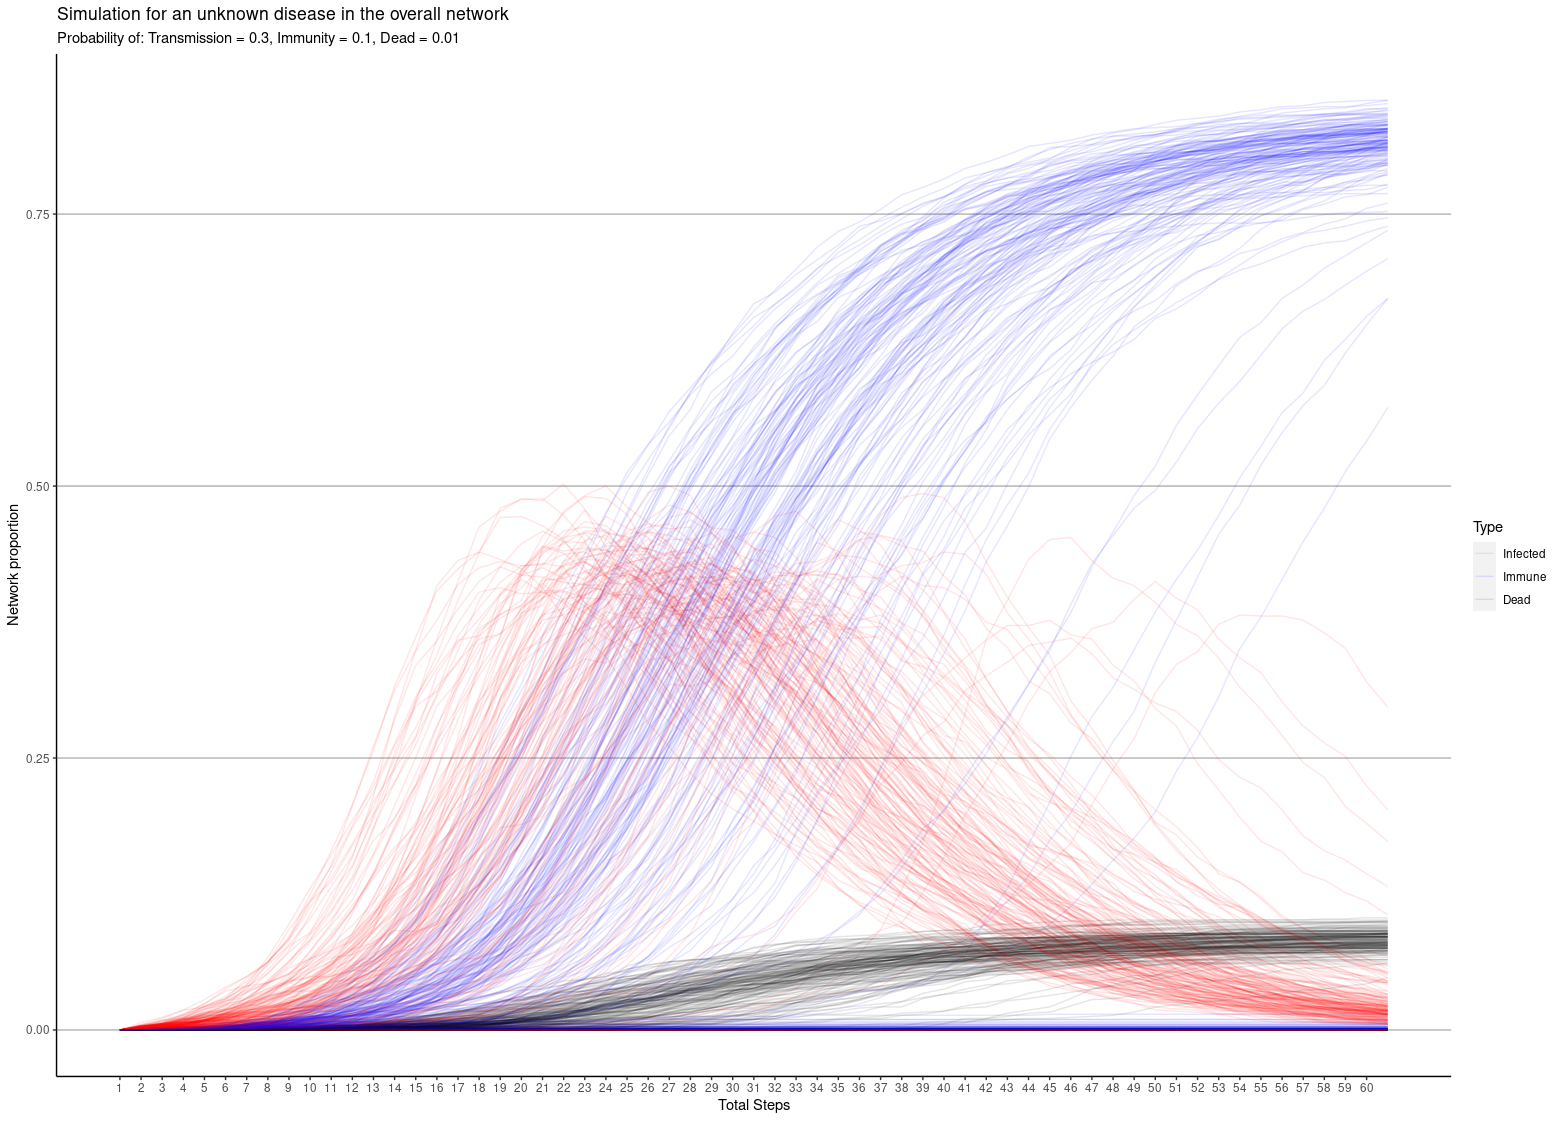
\includegraphics[width=0.95\linewidth]{figures/Networks/Simulations/Simulation_Nothing.png} 
        \caption{Simulation of the spread of an unknown disease in the network. In the x-axis, we have steps which is an arbitrary representation of time. In the y-axis the proportion of the network that each category has at any given time. Each red, blue, and red, line represent one of the 200 simulations. Red represents infected, Blue represents immunized, and Black represents dead.}
        \label{figure:simulationsA}
    \end{figure}   


For the second case (figure \ref{figure:simulationsB}), we introduce a vaccine. As expected the death rate drops dramatically, with about 23 students dying on average and an almost entirely immunized population in all cases. The peak of infections is reduced by more than half and is easier to predict when the worse time is going to happen.

    \begin{figure}[h!]
        \centering
            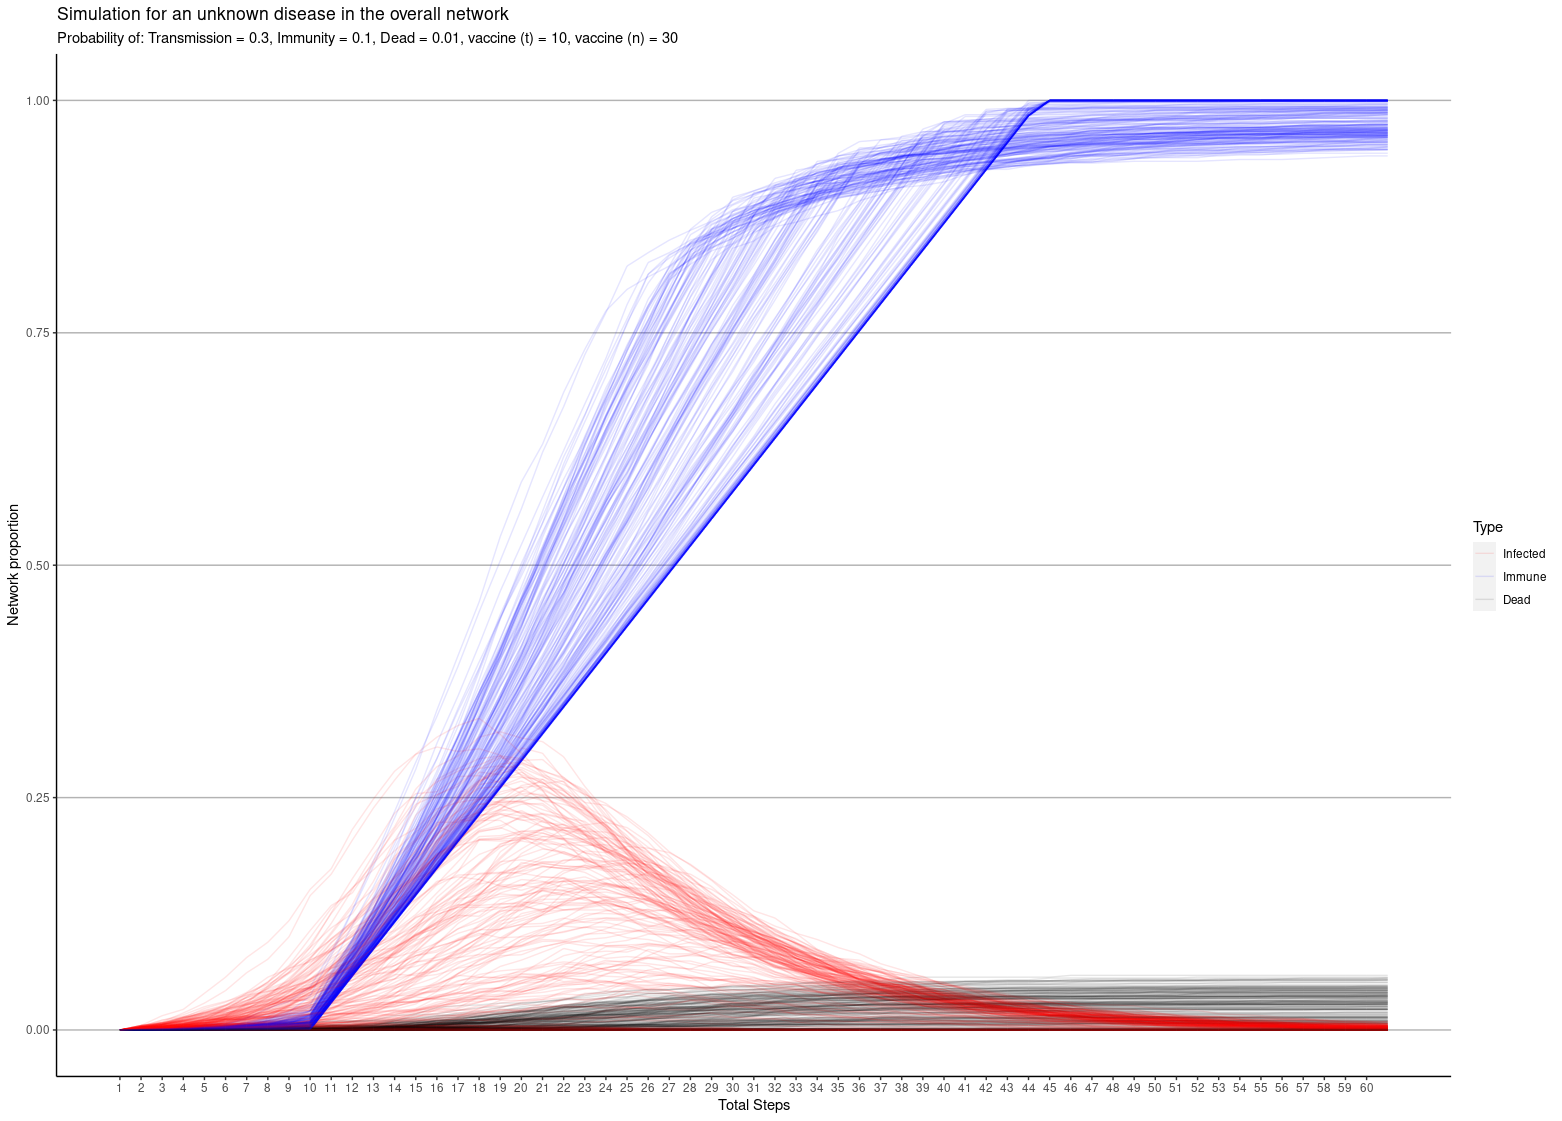
\includegraphics[width=0.95\linewidth]{figures/Networks/Simulations/Simulation_Vaccine_30.png} 
        \caption{Simulation of the spread of an unknown disease in the network. In the x-axis, we have the steps in time. In the y-axis the proportion of the network that each category has at any given time. Each red, blue, and red, line represent one of the 200 simulations. Red represents infected, Blue represents immunized, and Black represents dead. A vaccine is introduced at t = 10 which suddenly spikes the immunization ratio and lower dead rate}
        \label{figure:simulationsB}
    \end{figure}  

The rest of the cases produce similar figures with the slope of immunity being a bit more or less pronounced. The best results are when we apply the vaccine to people connecting subnetworks, in that way, we can isolate the disease very quickly. Notice that the number of deaths is lower when we immunize first people connecting sub-networks together (n = 16), rather than just giving it first to the most well-connected people (n = 18), which suggests that having prior knowledge of the network topology can help to safe lives.

    %\begin{figure}[h!]
     %   \centering
      %      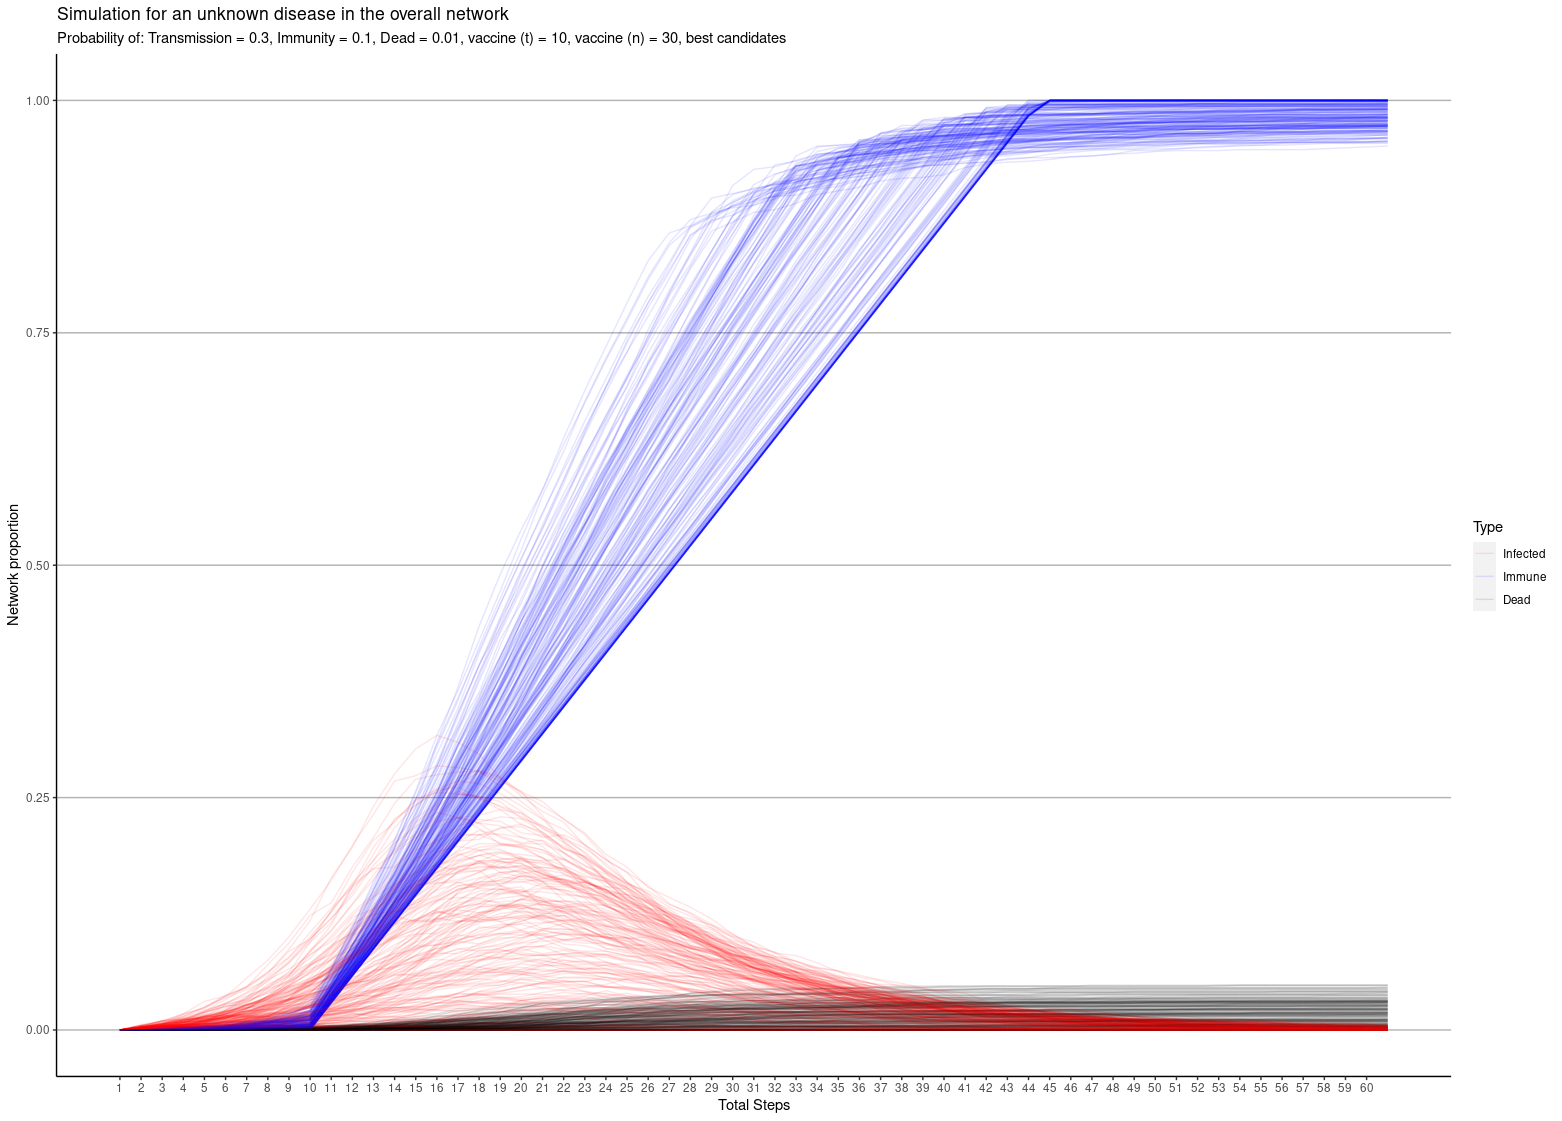
\includegraphics[width=0.95\linewidth]{figures/Networks/Simulations/Simulation_Best_30.png} 
       % \caption{Simulation of the spread of an unknown disease in the network. In the x-axis, we have the steps in time. In the y-axis the proportion of the network that each category has at any given time. Each red, blue, and red, line represent one of the 200 simulations. Red represents infected, Blue represents immunized, and Black represents dead. A vaccine is introduced at t = 10, but is given to the highest connected students first}
        %\label{figure:simulationsC}
    %\end{figure}  





%Nothing

%[1] "-------------"
%[1] "Mean Immunity:       0.621459537572254 +- 0.345102052201196"
%[1] "Mean Dead:           0.0629624277456647 +- 0.0357281205280136"
%[1] "Mean max infections: 0.327105009633911 +- 0.182383294477629"
%[1] "at time:             23.2 +- 10.6568212519484"

% Vaccine 30
%[1] "-------------"
%[1] "Mean Immunity:       0.978468208092486 +- 0.017343662559995"
%[1] "Mean Dead:           0.0216955684007707 +- 0.0177364552599782"
%[1] "Mean max infections: 0.122263969171484 +- 0.0998856407568371"
%[1] "at time:             19.145 +- 7.66929366543185"


% Best 30
%1] "-------------"
%[1] "Mean Immunity:       0.983482658959538 +- 0.0133188475582221"
%[1] "Mean Dead:           0.0170857418111753 +- 0.013902438604357"
%[1] "Mean max infections: 0.100770712909441 +- 0.0815998034228179"
%[1] "at time:             17.47 +- 6.00662113733147"

% Best Betweeness 30
%[1] "-------------"
%[1] "Mean Immunity:       0.985134874759152 +- 0.0134353361062699"
%[1] "Mean Dead:           0.0153131021194605 +- 0.0139325719338487"
%[1] "Mean max infections: 0.0920905587668593 +- 0.0832644828832967"
%[1] "at time:             15.855 +- 6.96754680951004"

% Best Closeness 30
% [1] "-------------"
% [1] "Mean Immunity:       0.983111753371869 +- 0.0150894772699903"
% [1] "Mean Dead:           0.0169701348747592 +- 0.0154606868655294"
% [1] "Mean max infections: 0.0909826589595376 +- 0.0851839777319293"
% [1] "at time:             17.205 +- 8.70354718883868"

% Best Eigen 30
% [1] "-------------"
% [1] "Mean Immunity:       0.975375722543353 +- 0.0174053731268066"
% [1] "Mean Dead:           0.0248603082851638 +- 0.017978236810753"
% [1] "Mean max infections: 0.139797687861272 +- 0.102859340836389"
% [1] "at time:             19.345 +- 9.04516723180154"
    
We also have the option of running this type of analysis against any layout of any network and making a comprehensive video simulation. This can be seen in figure \ref{fig:networkVideo}.

\begin{figure}[ht]
    \centering
    \begin{minipage}[b]{0.45\linewidth}
        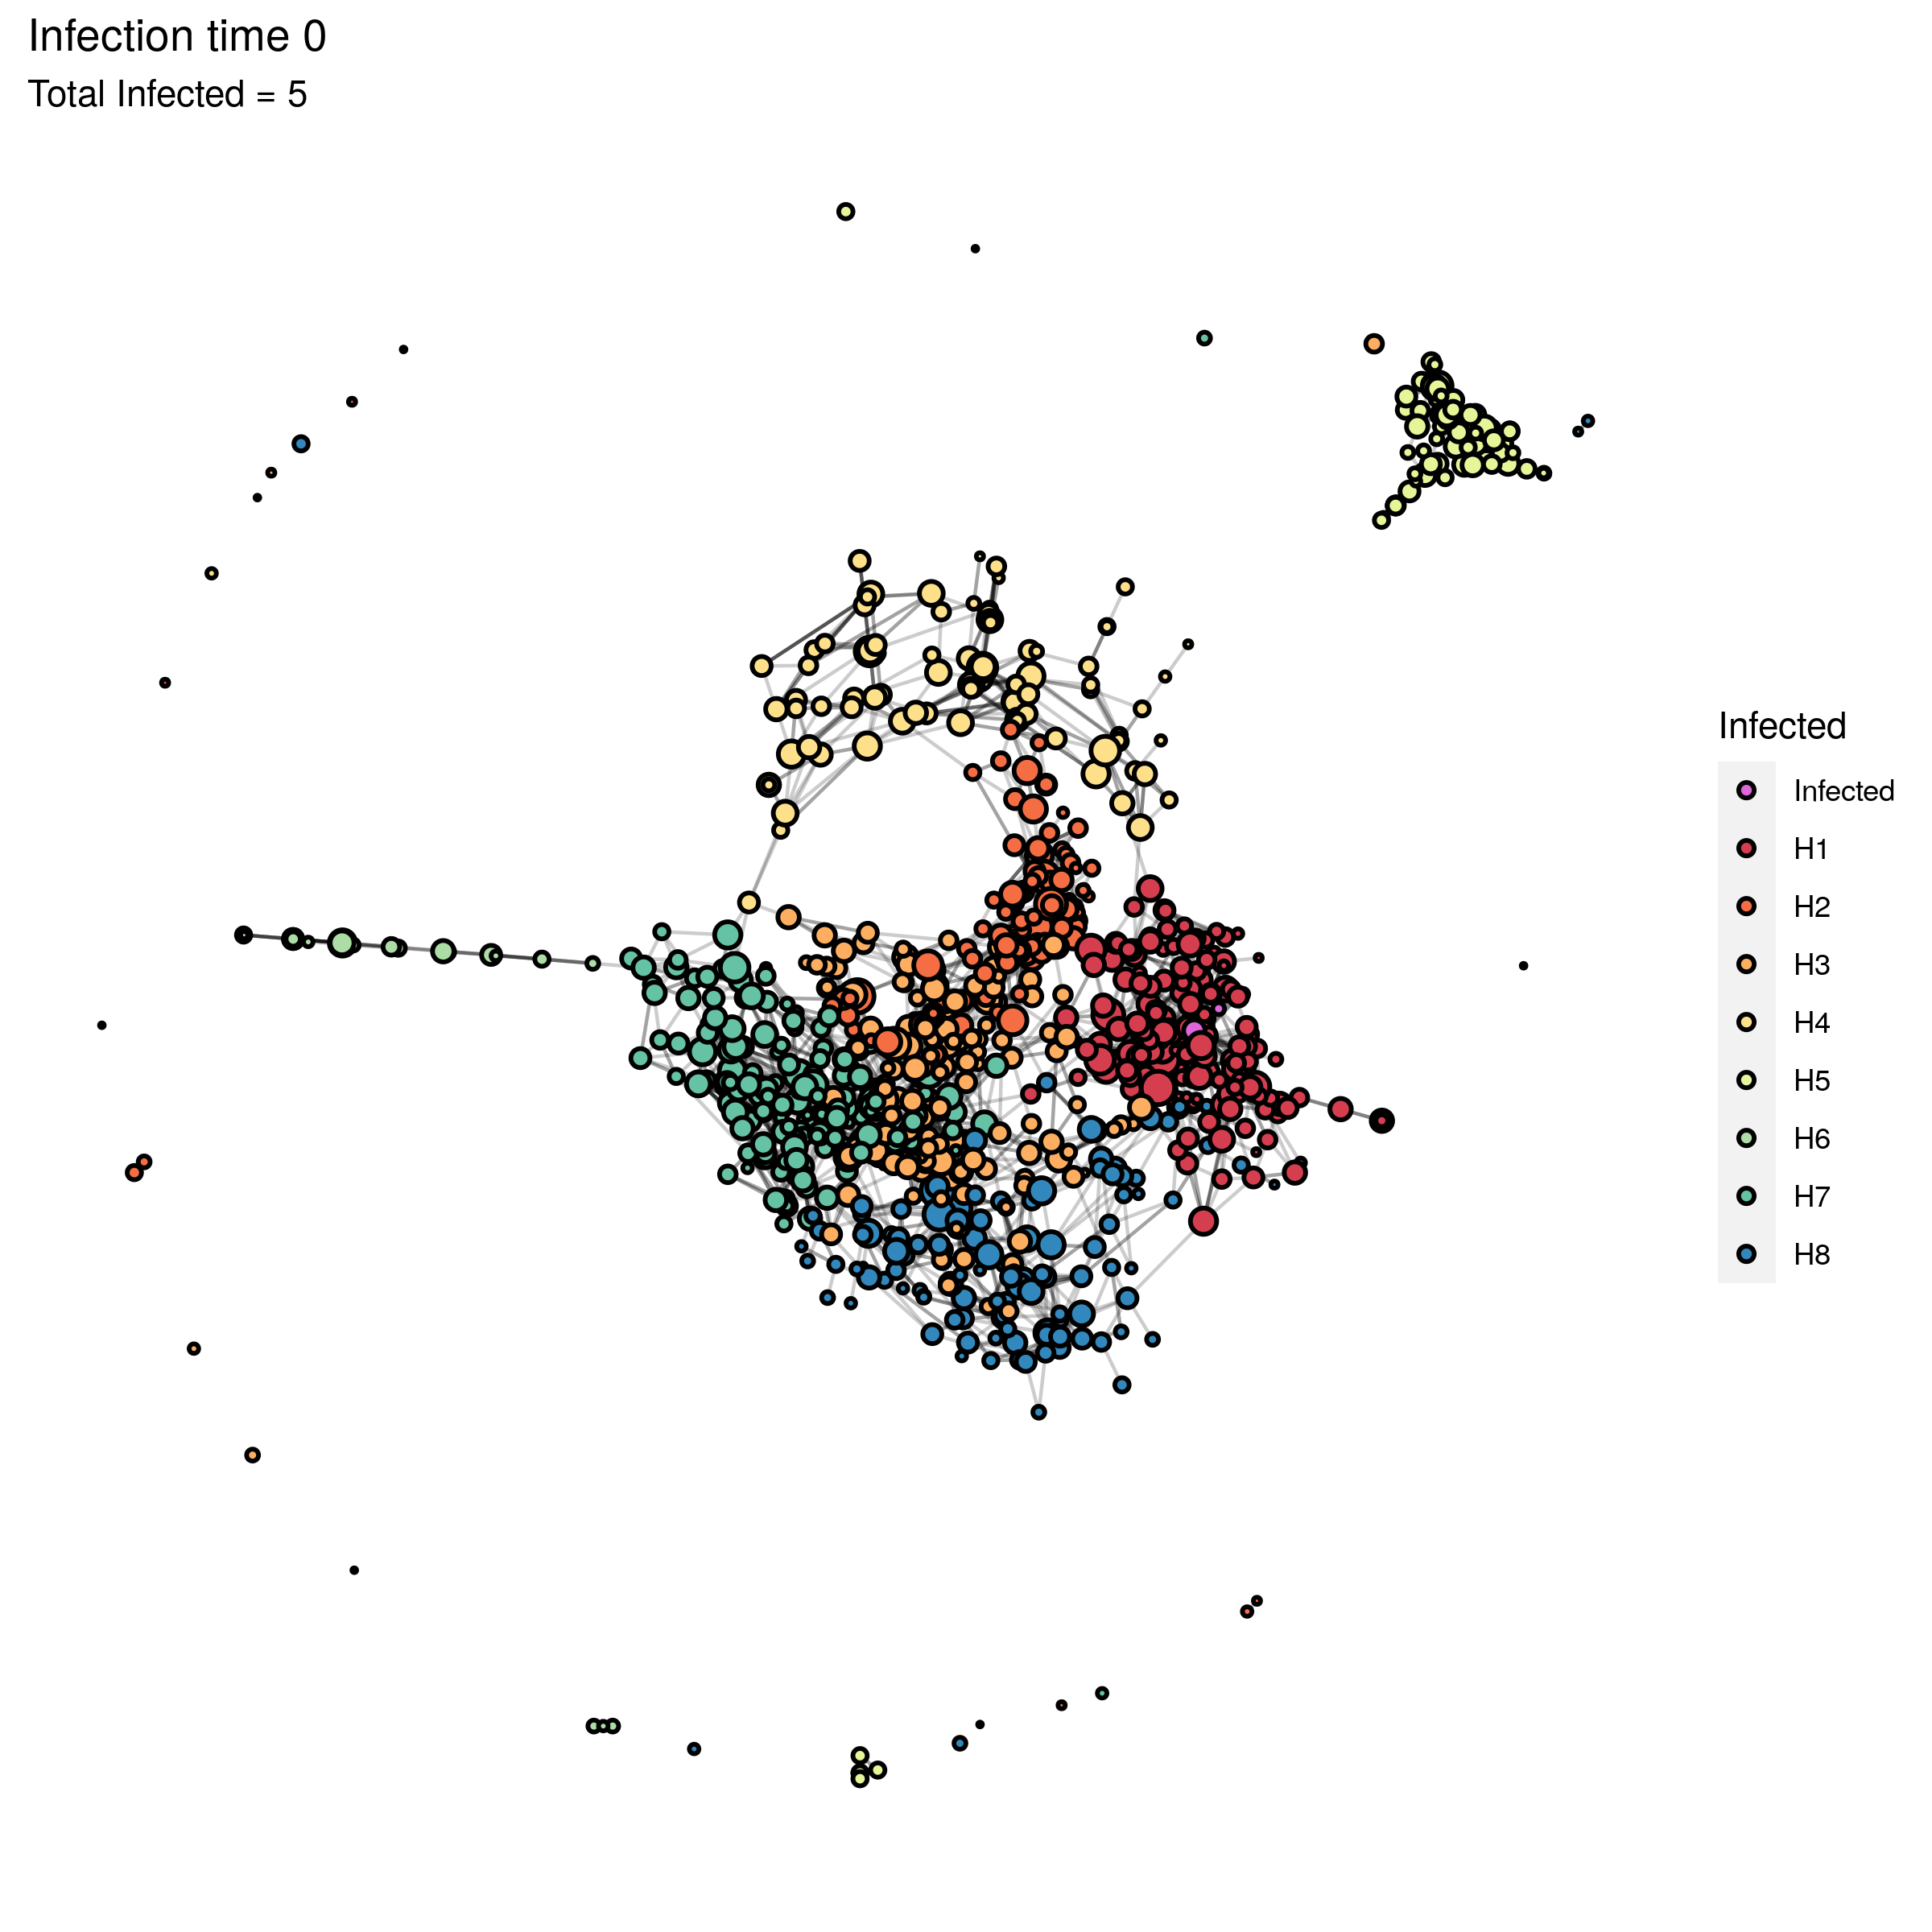
\includegraphics[width=\linewidth]{figures/Networks/Video/Graph_Infection_0_Infected___manual.png}
        \caption{a}
    \end{minipage}
    \hfill
    \begin{minipage}[b]{0.45\linewidth}
        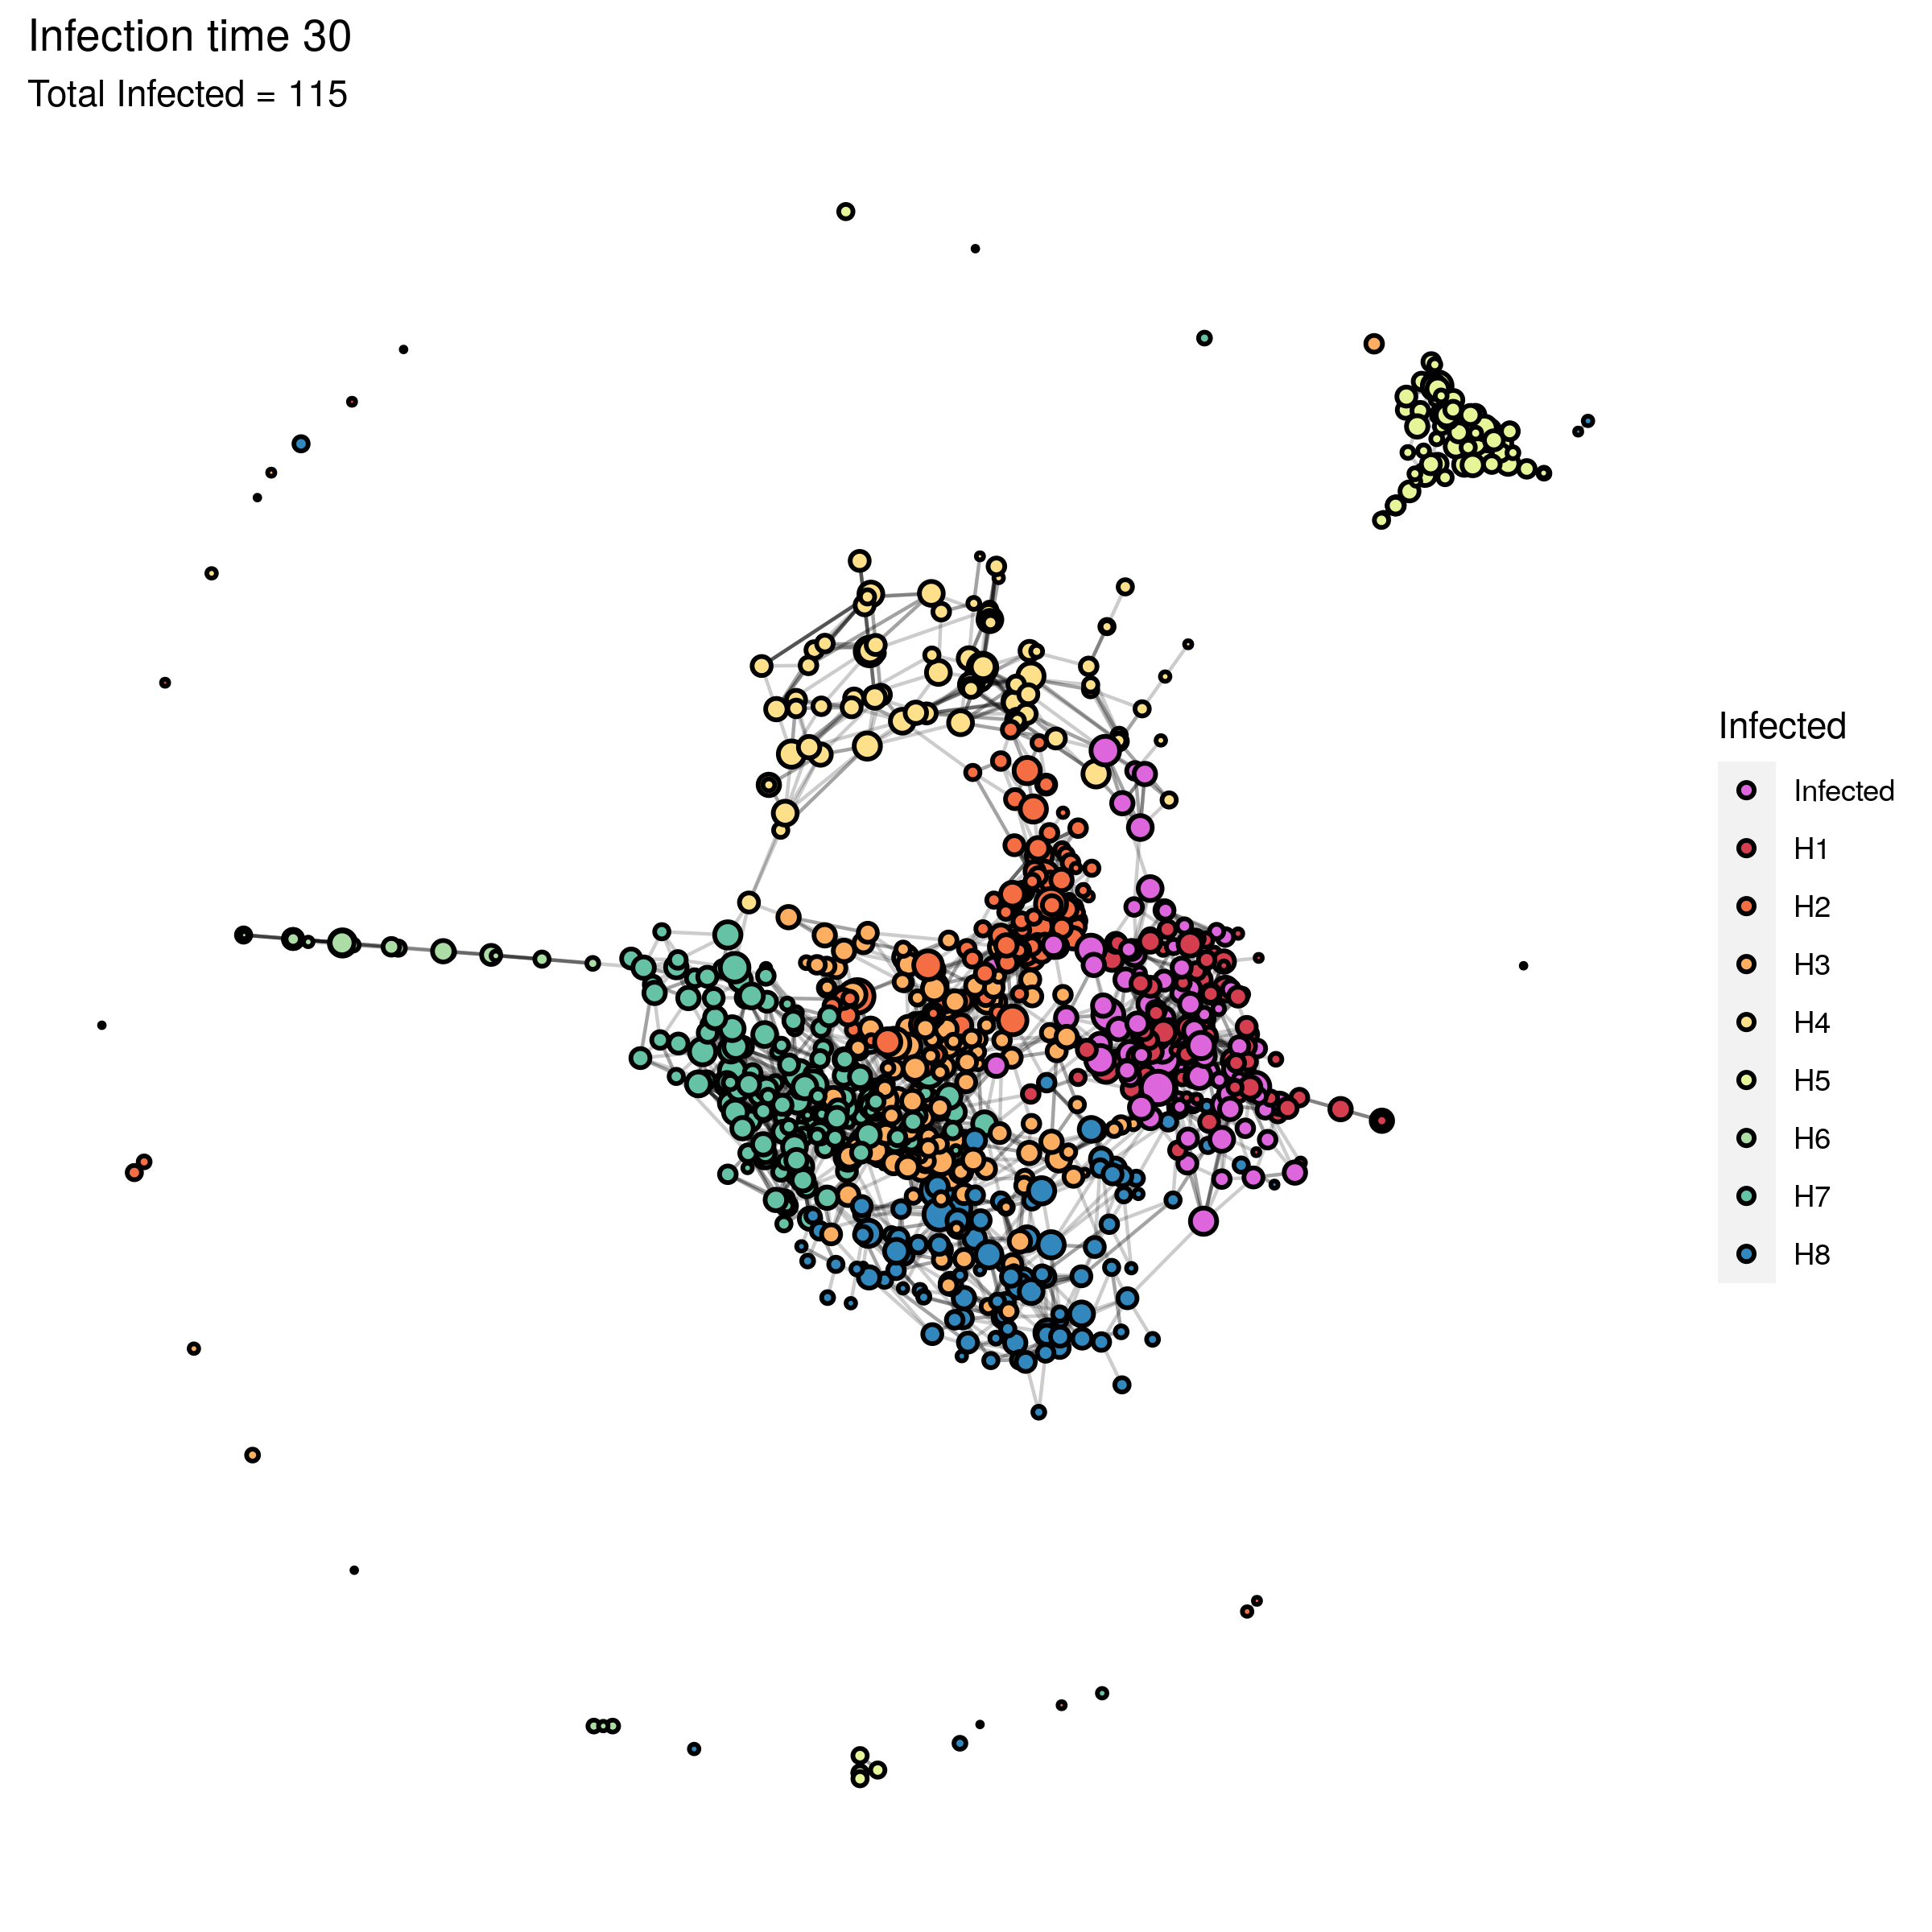
\includegraphics[width=\linewidth]{figures/Networks/Video/Graph_Infection_30_Infected___manual.png}
        \caption{b}
    \end{minipage}
    \vfill
    \begin{minipage}[b]{0.45\linewidth}
        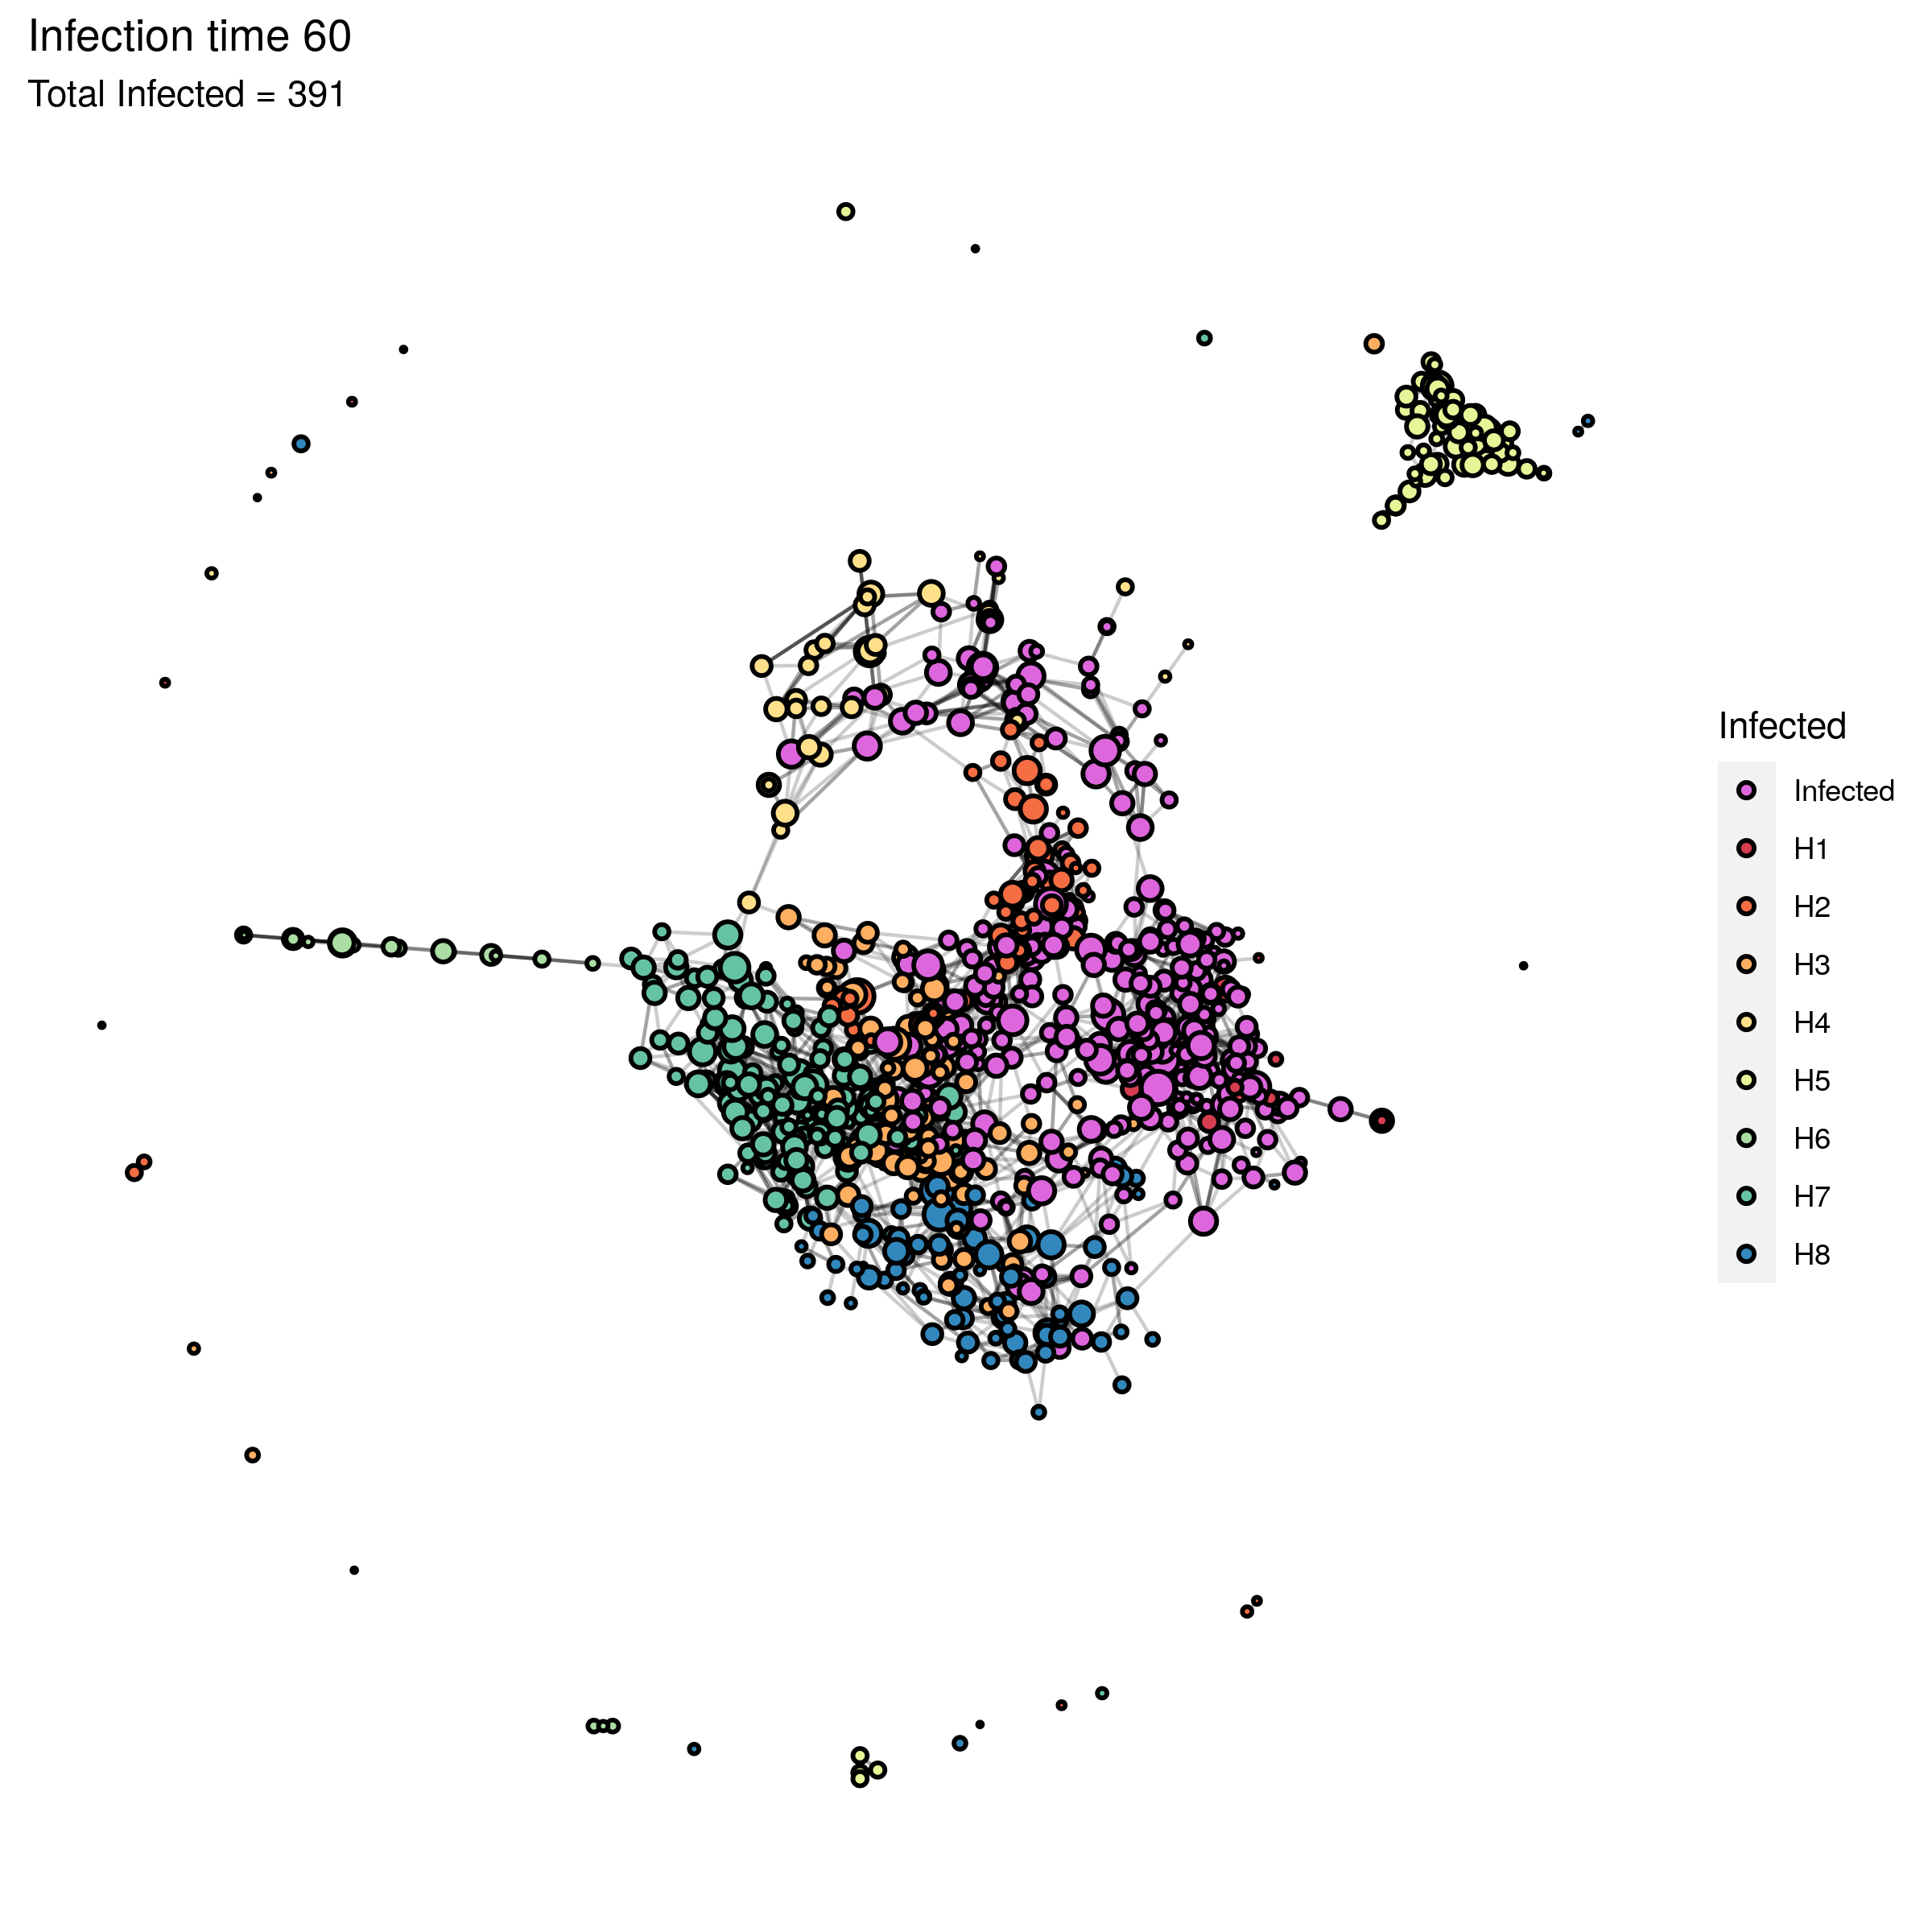
\includegraphics[width=\linewidth]{figures/Networks/Video/Graph_Infection_60_Infected___manual.png}
        \caption{c}
    \end{minipage}
    \hfill
    \begin{minipage}[b]{0.45\linewidth}
        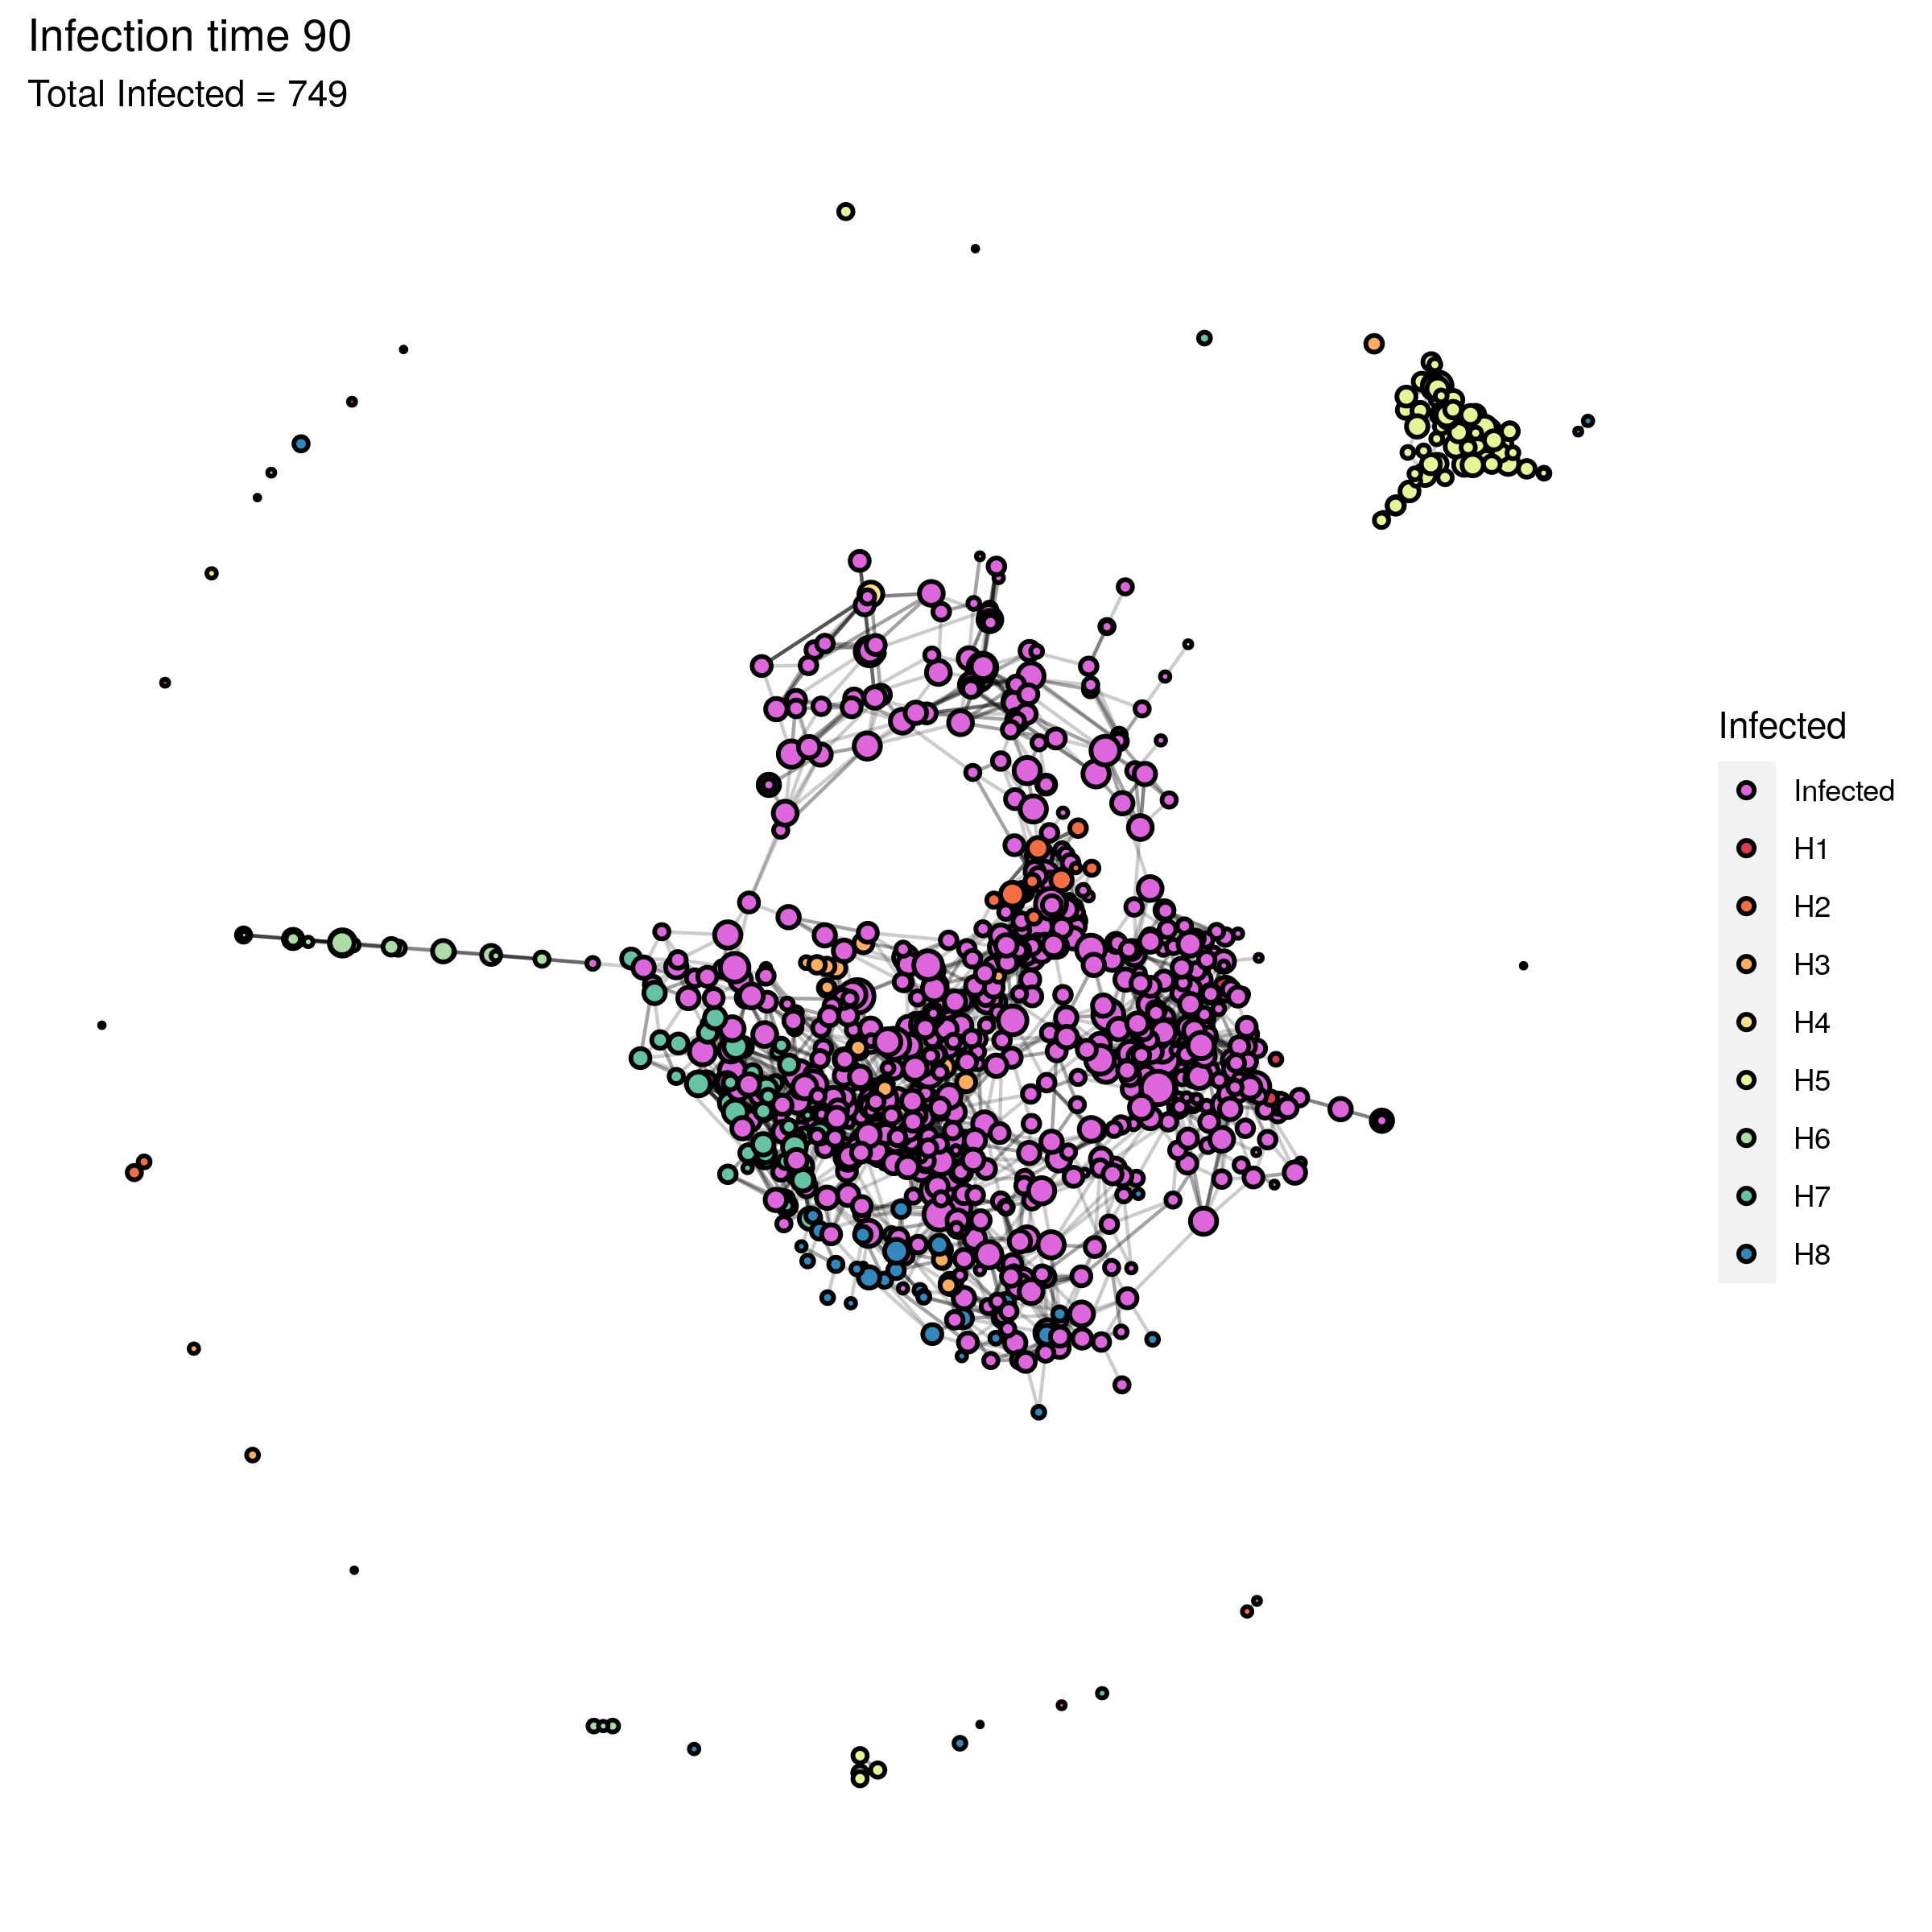
\includegraphics[width=\linewidth]{figures/Networks/Video/Graph_Infection_90_Infected___manual.png}
        \caption{d}
    \end{minipage}
    \caption{A simulation of a disease advancing through the School Network using an MDS layout. Each sub-figure represents the disease advance after (a) 0 steps with 5 random initials infected (b) 30 steps (c) 60 steps (d) 90 steps. Infected people are highlighted in violet, and each school is highlighted in a different color. The disease starts in H1 and spread to closer contacts. H5 and all isolated components are spared because is not connected and thus impossible to reach in this particular model. The complete video of the simulation can be found at \url{https://github.com/uit-hdl/mimisbrunnr/blob/main/results/network/simulation.mp4}}
    \label{fig:networkVideo}
\end{figure}


%\begin{figure}
 %   \centering
  %  \subfigure[]{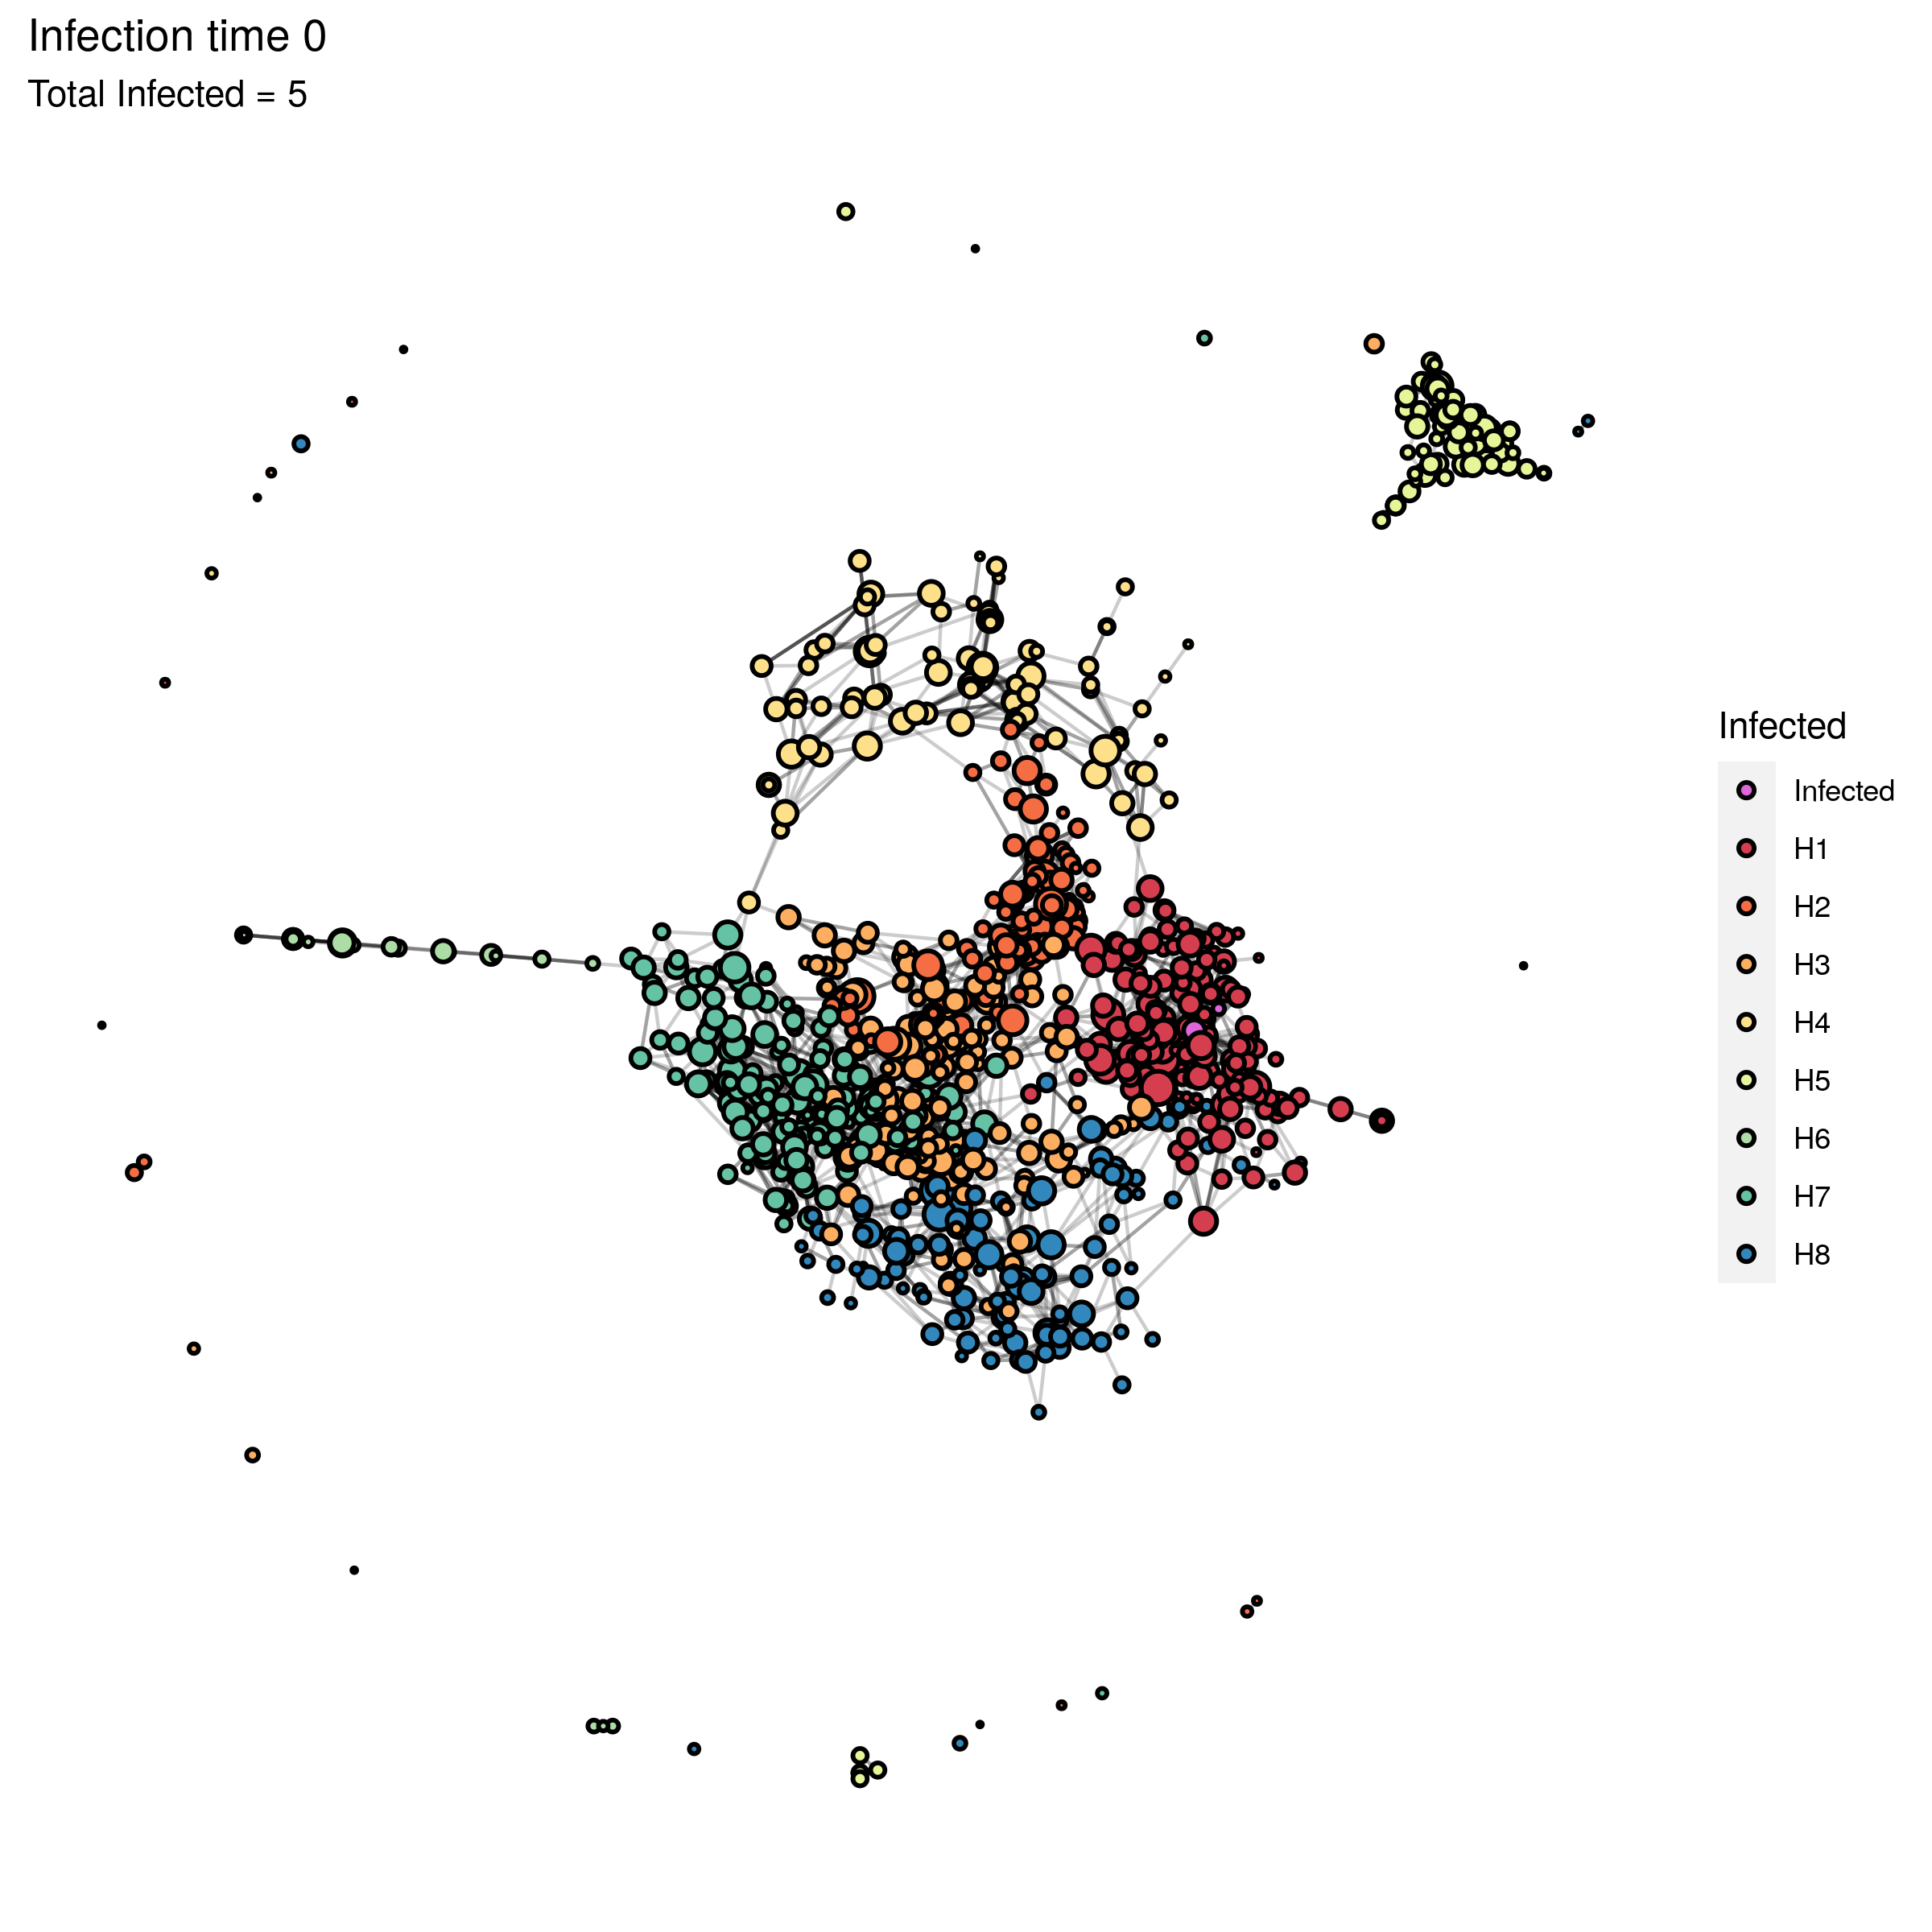
\includegraphics[width=0.45\textwidth]{figures/Networks/Video/Graph_Infection_0_Infected___manual.png}} 
   % \subfigure[]{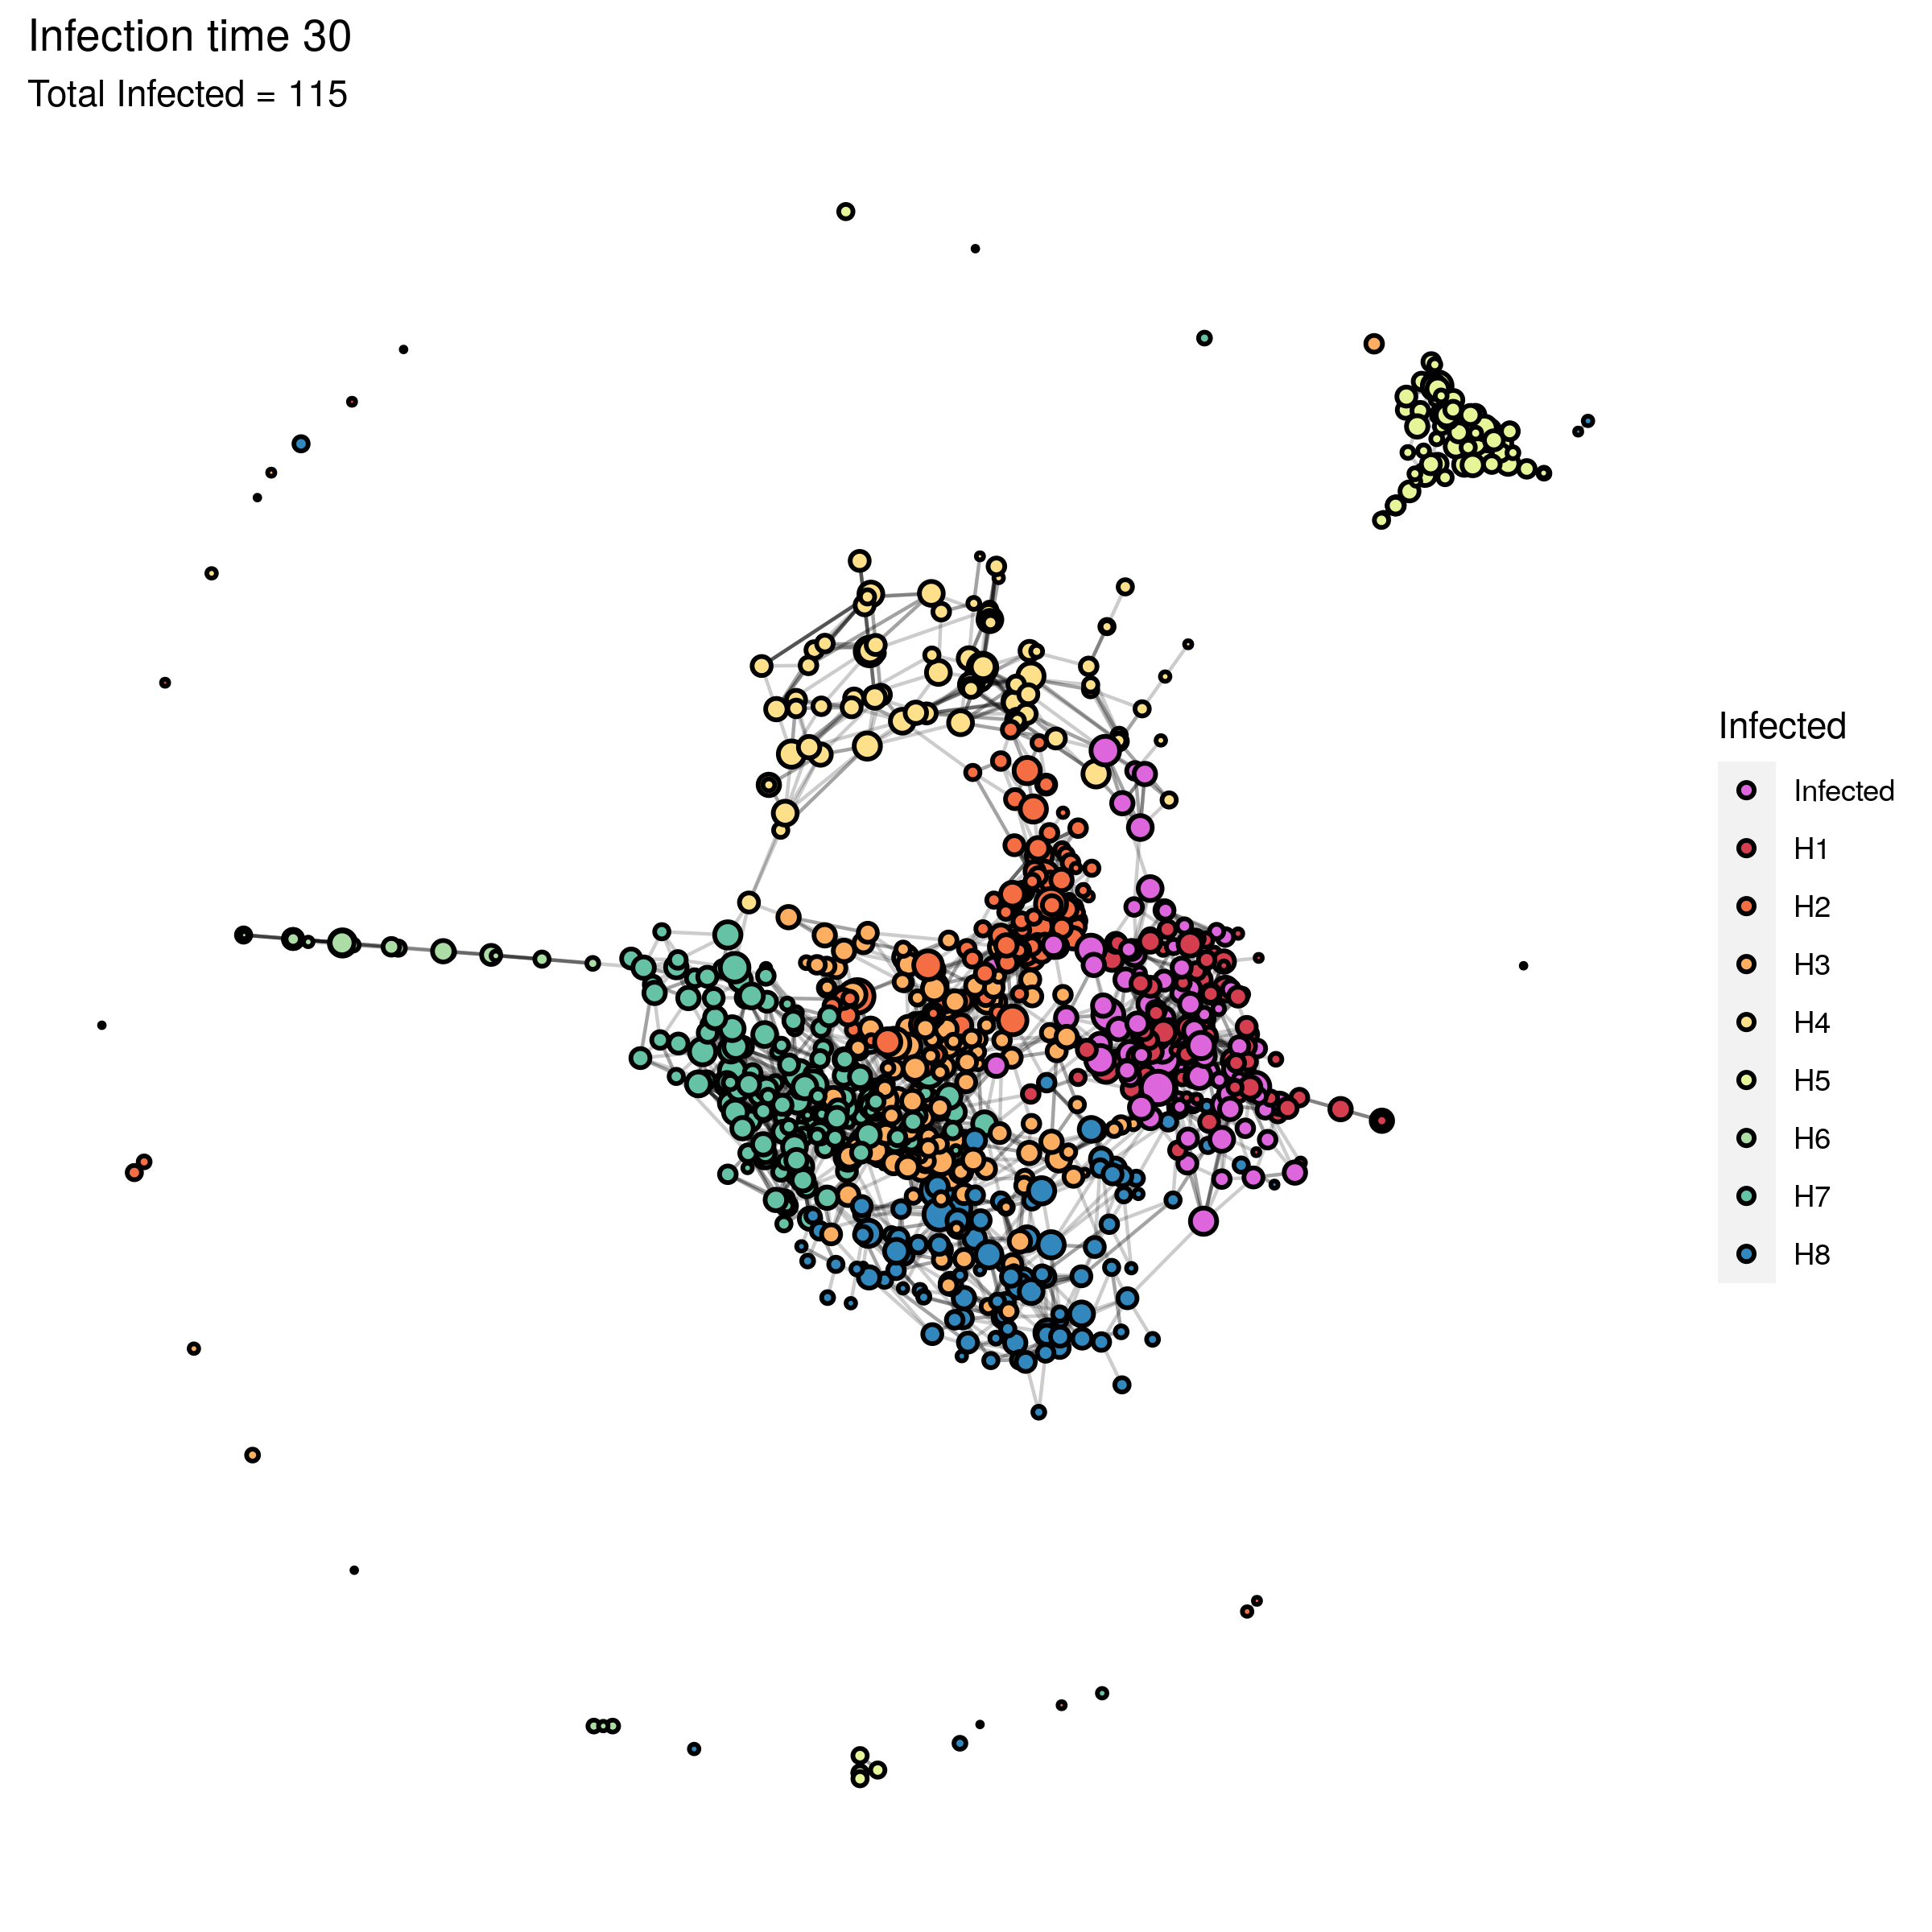
\includegraphics[width=0.45\textwidth]{figures/Networks/Video/Graph_Infection_30_Infected___manual.png}} 
    %\subfigure[]{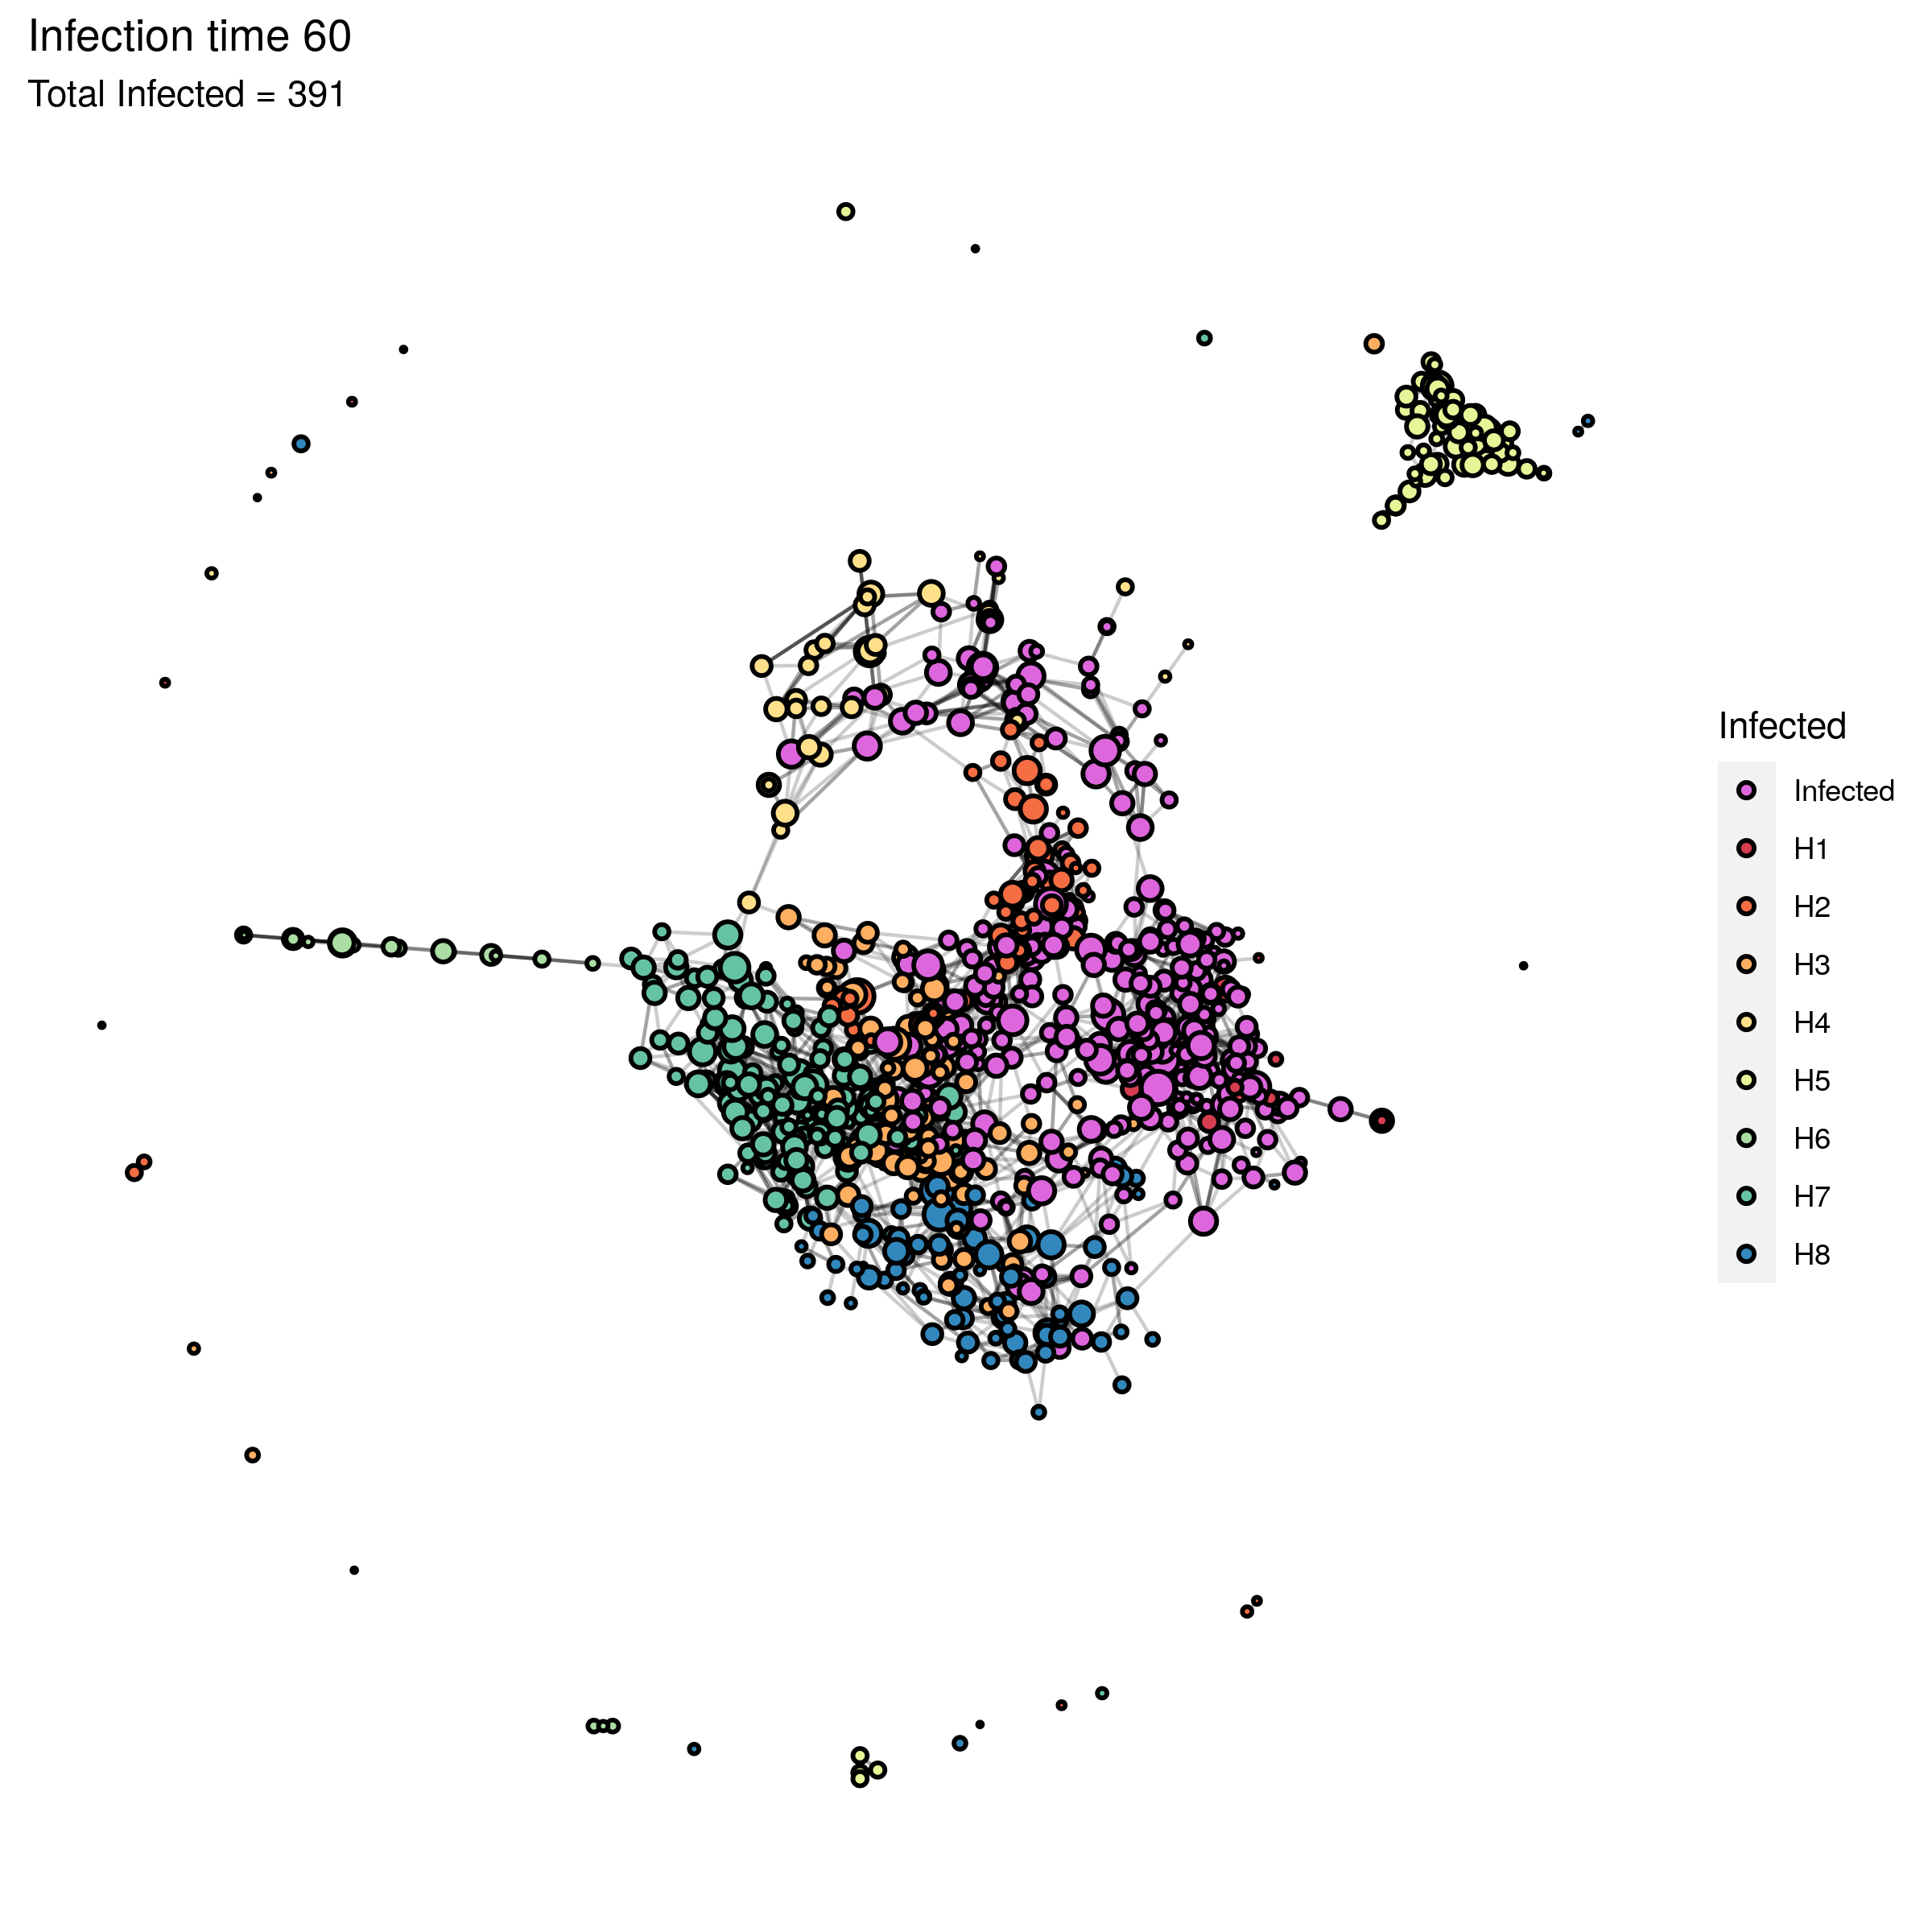
\includegraphics[width=0.45\textwidth]{figures/Networks/Video/Graph_Infection_60_Infected___manual.png}}
    %\subfigure[]{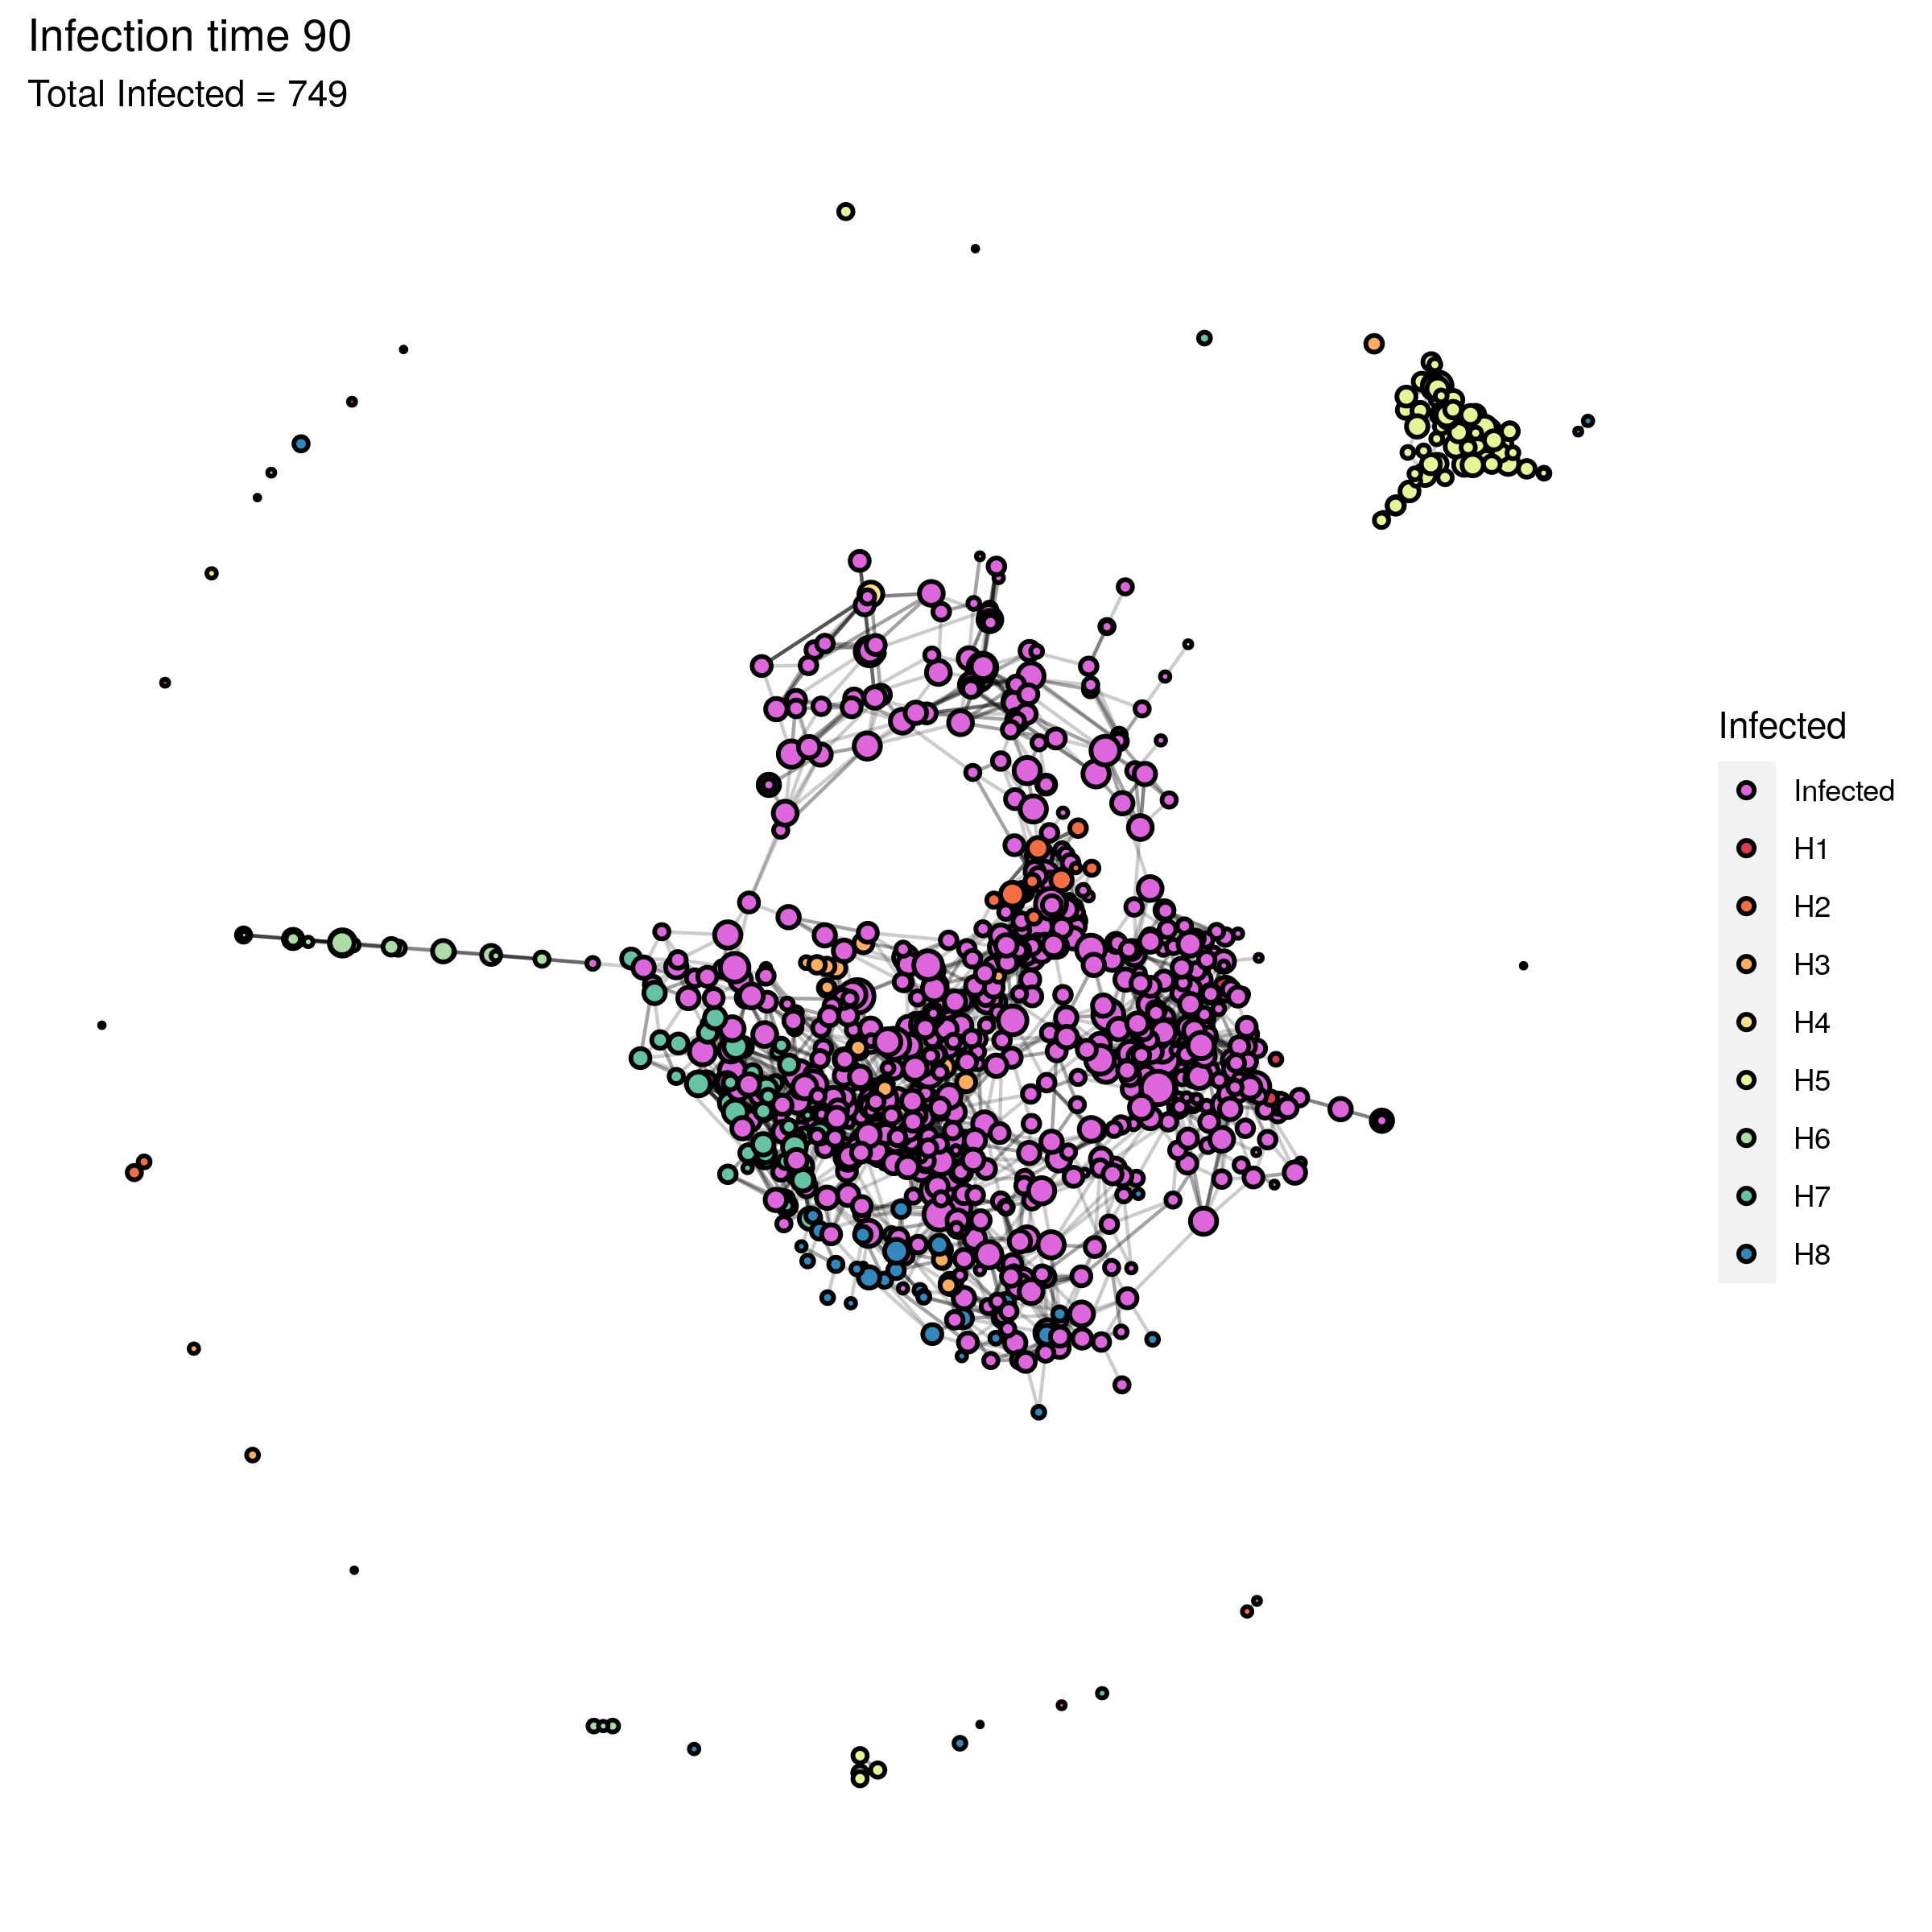
\includegraphics[width=0.45\textwidth]{figures/Networks/Video/Graph_Infection_90_Infected___manual.png}}
    %\caption{A simulation of a disease advancing through the School Network using a MDS layout. Each sub-figure represent the disease advance after (a) 0 steps (b) 30 steps (c) 60 steps (d) 90 steps. Infected people are highlighted in violet, each school is highlighted in a different color. The disease start in H1 and spread to closer contacts. H5 is spared because is not connected and thus impossible to reach in this particular model. The complete video of the simulation can be found at \url{https://github.com/uit-hdl/mimisbrunnr/blob/main/results/network/simulation.mp4}}
    %\label{fig:networkVideo}
%\end{figure}

\section{Final}

You can learn more about how to draw a network in Paper F \ref{chapter:chapterListPapers}. Furthermore, all the code which generates figures and tables for this thesis is available in our GitHub repository. Several other good and free resources exist online %https://bdpedigo.github.io/networks-course/plotting_networks.html
